\documentclass[10pt]{esda}
\font\titlefont=cmss12 at 40pt
\font\authorfont=cmr10 at 30pt

\title{}
\author{}
\date{}

\header{}

%\category{PIC2 Report}
\category{Master Thesis}

\input{color}

%\usepackage{setspace}
%\doublespacing

\raggedbottom

\usepackage{helvet}
\renewcommand{\familydefault}{\sfdefault}

\usepackage{setspace}
\setstretch{1.5}

\usepackage{titlesec}
\titleformat{\section}
{\fontsize{28}{20}\selectfont\bfseries}{\thesection}{1em}{}

\begin{document}

%\begin{singlespace}
%\vspace{-1cm}
\includegraphics[bb=9.5cm 11cm 0cm 0cm,scale=0.29]{ist_logo.pdf}
%\vspace{2.5cm}

%{\let\newpage\relax\maketitle}
%\pagenumbering{gobble}
\thispagestyle{empty}

\vspace{2.5cm}

\begin{figure}[H]
  \centering
  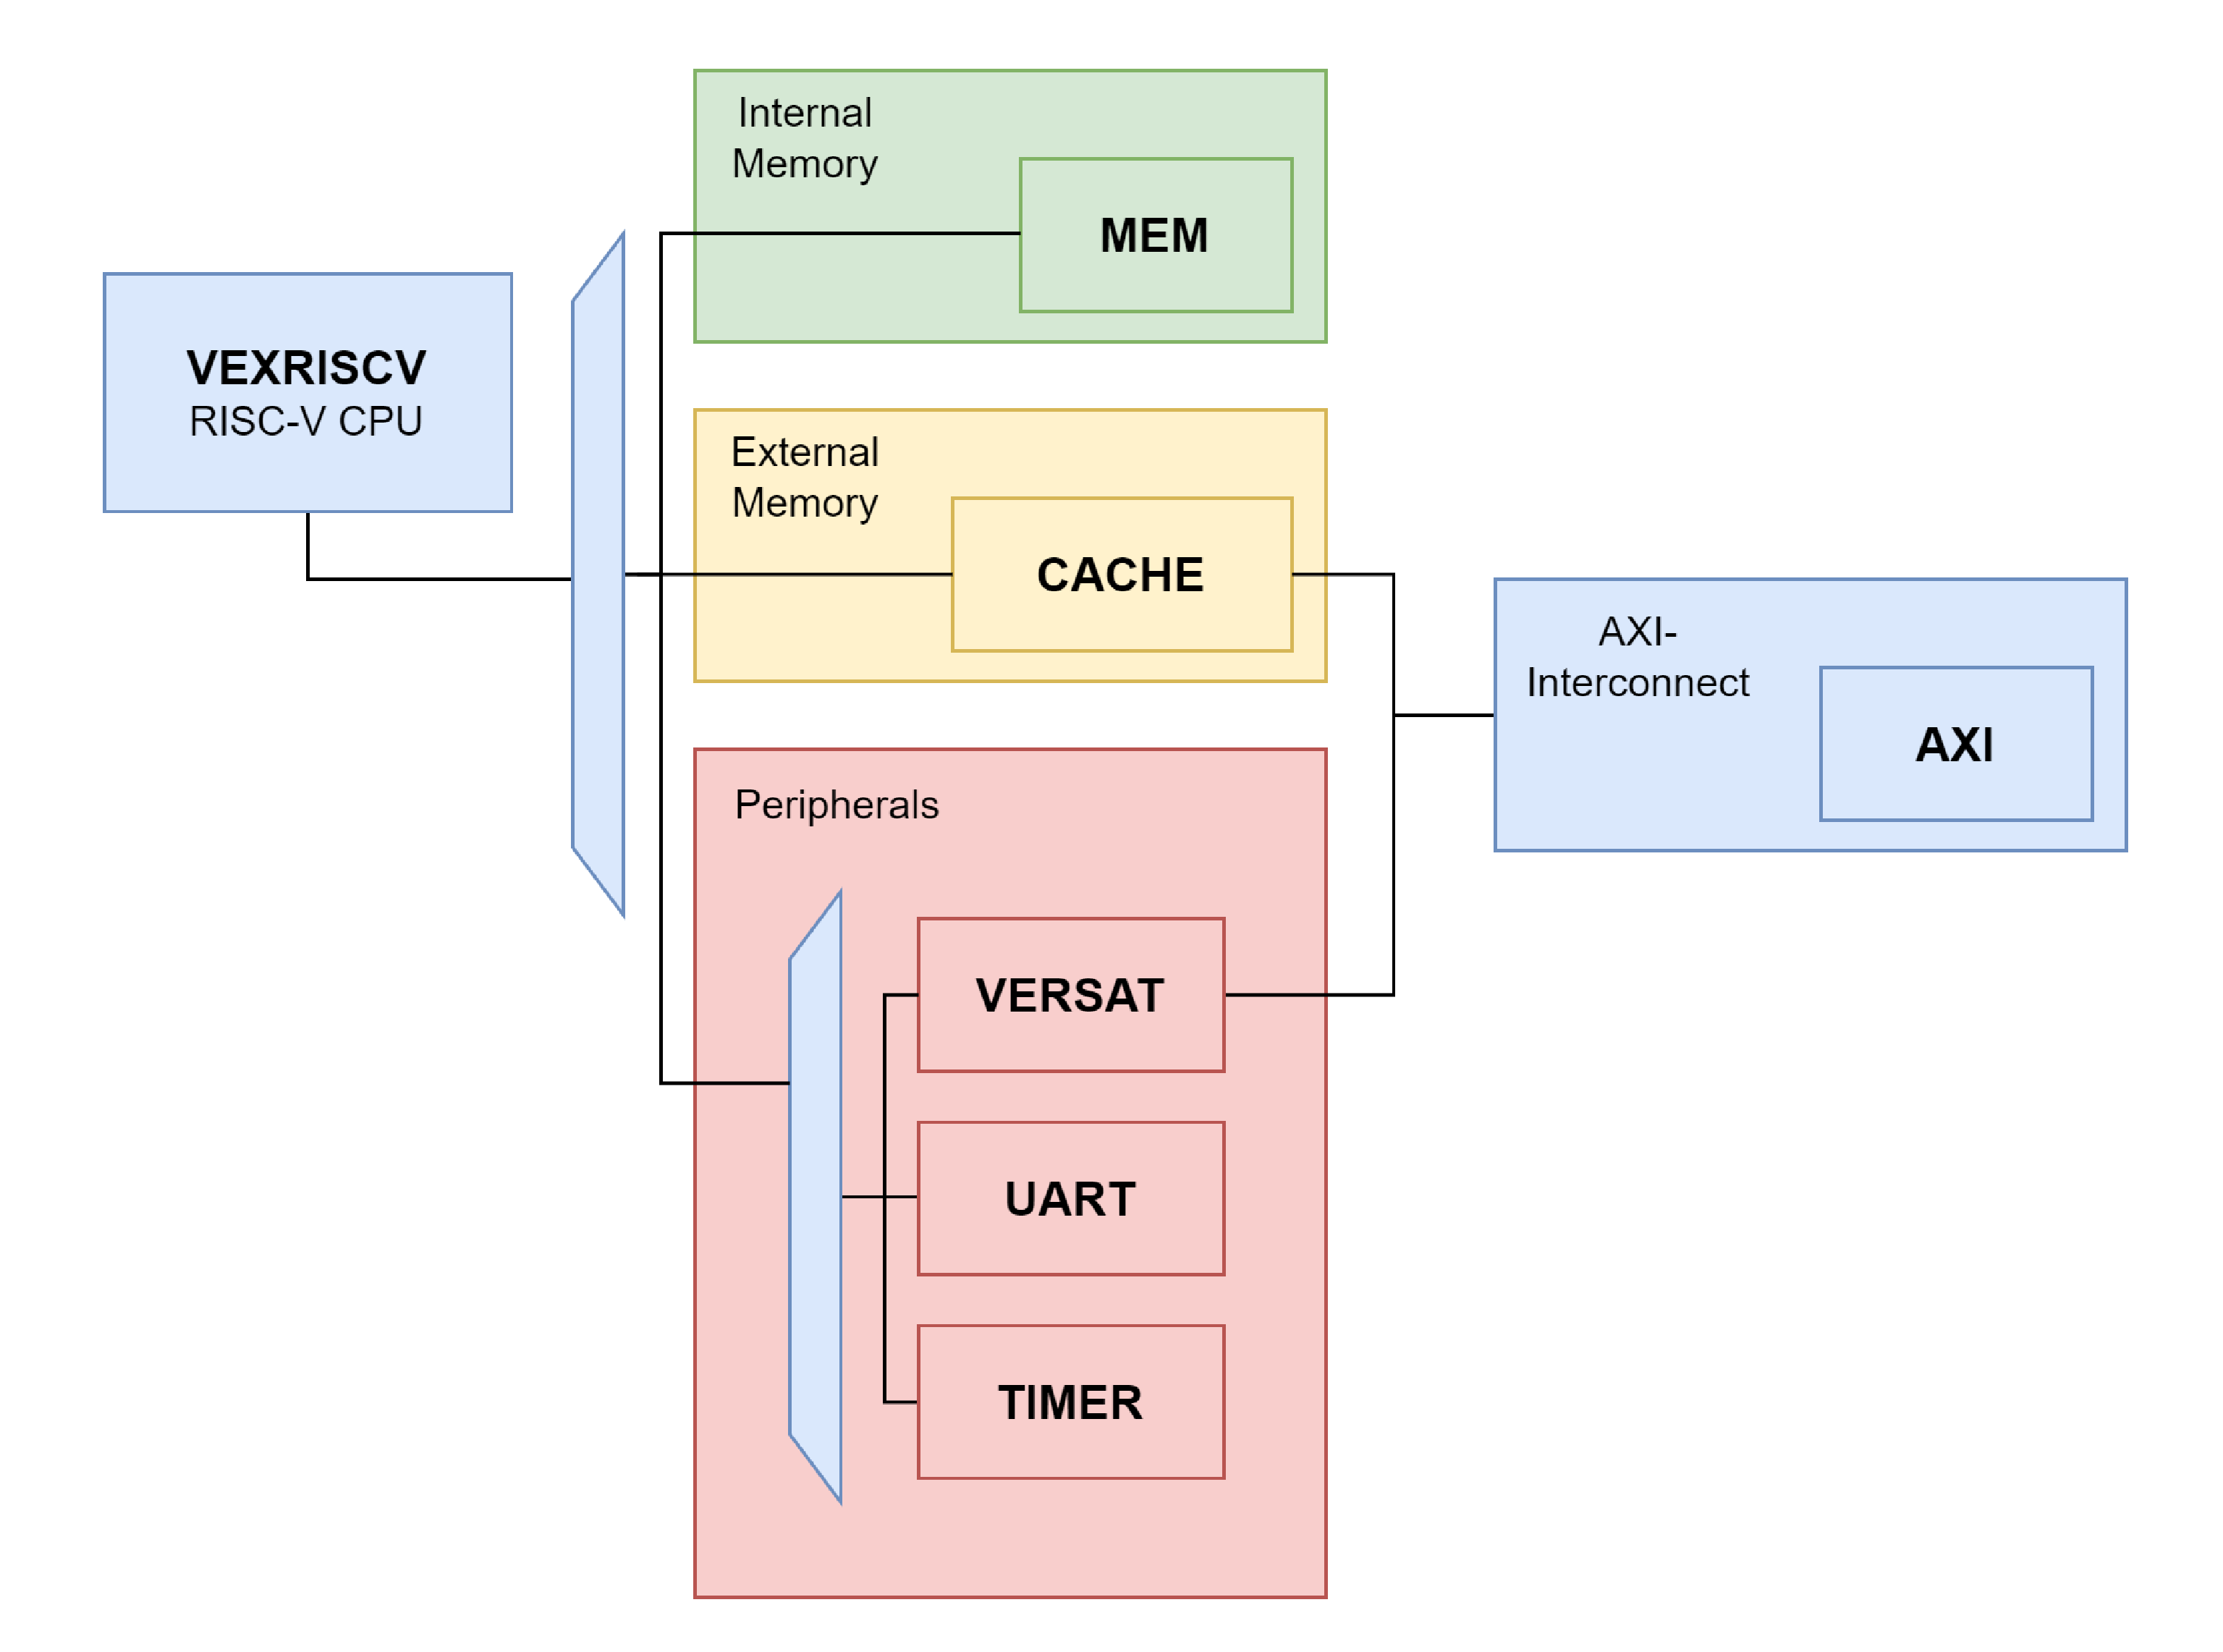
\includegraphics[scale=0.3]{iob2.pdf}
\end{figure}


\begin{onehalfspace}

\begin{center}
\begin{Large}
  {\bf \Large {MPEG1/2 layers I/II encoder using \\ a RISC-V processor and hardware accelerators}}\\
  \vspace{1cm}
  {\bf \large Tiago Alves da Silva}\\
  \vspace{1cm}
  \normalsize {Thesis to obtain the Master of Science Degree in}\\
  \vspace{0.5cm}
  {\bf \Large {Electrical and Computer Engineering}}\\
  \vspace{1cm}
  \normalsize {Supervisor: Prof. Doutor José João Henriques Teixeira de Sousa}\\
  \vspace{1cm}
  {\bf \large Examination Committee}\\
  \vspace{1cm}
  \normalsize {Chairperson: Prof. Doutora Teresa Maria Canavarro Menéres Mendes de Almeida}\\
  \normalsize {Supervisor: Prof. Doutor José João Henriques Teixeira de Sousa}\\
  \normalsize {Member of the Committee: Prof. Doutor Marcelino Bicho dos Santos}\\

  \vspace{1cm}
  %{\bf \date{\today} }
  {\bf \large October 2023 }
\end{Large}
\end{center}

\end{onehalfspace}
%\linespread{1.25}
%\begin{doublespacing}

\clearpage
\thispagestyle{empty}
\cleardoublepage


\pagenumbering{roman}
\section*{Declaration}
\hspace{0.4cm} I declare that this document is an original work of my own authorship and that it fulfills all the requirements of the Code of Conduct and Good Practices of the Universidade de Lisboa. 

\cleardoublepage
\section*{Acknowledgements}
\hspace{0.4cm} I want to thank Professor José de Sousa for for his invaluable guidance and support during my master's thesis. As my supervisor, he played a significant role in helping me understand the research process, providing valuable insights on what needed to be done and how to approach it. His professionalism and high standards were instrumental in this work.

I want to express my gratitude to Rúben Teixeira for his assistance in enhancing my understanding of the hardware accelerator matter. His guidance on the practical aspects of this work, including optimization techniques, was immensely helpful, especially during the latter stages.

I am also deeply thankful to my family for their unwavering support and encouragement. Their constant belief in me and encouragement to give my best has been a motivating force throughout my academic journey.


\cleardoublepage
\section*{Resumo}
\hspace{0.4cm} O Grupo de Especialistas em Imagem em Movimento (MPEG) foi crucial na transição do áudio analógico para o digital. O MPEG suporta a Transmissão de Áudio Digital (DAB), com o MPEG-1 Audio a ser um formato de áudio globalmente popular. O MPEG inclui esquemas de codificação como a Camada I para baixa complexidade e a Camada II para aplicações de um-para-muitos.
No desenvolvimento de Sistemas num Chip (SoC), equilibrar o desempenho e o custo é desafiador. Esta tese apresenta um codificador de Áudio MPEG-1/2 de Camada II de vírgula flutuante, oferecendo alta precisão num mercado com recursos de Propriedade Intelectual (IP) limitados.
A arquitetura de software apresenta a Unidade Central de Processamento (CPU) \textit{VexRiscv} num cenário IOb-SoC, utilizando o algoritmo \textit{TwoLAME}. São aplicadas otimizações de software. A análise de desempenho com o periférico \textit{TIMER} destaca o impacto da função \textit{psycho\_3\_threshold}, representando 37\% a 64\% do tempo de execução.
No lado de hardware, o \textit{Versat} é integrado no IOb-SoC para acelerar a função \textit{psycho\_3\_threshold}, implicando a expansão da Advanced eXtensible Interface (AXI). Dois aceleradores, \textit{spectrum\_search} e \textit{masking\_threshold}, abordam partes da função \textit{psycho\_3\_threshold}. A implementação em campo de matriz de portas programável (FPGA) mostra um aumento nas Tabelas de Consulta Total (LUTs), Flip-Flops e Blocos de Processador de Sinais Digitais (DSP).
O tempo de execução é significativamente reduzido com o acelerador \textit{spectrum\_search}.
Comparando com os requisitos de codificação em tempo real, o primeiro ficheiro com menos frames fica ligeiramente aquém, enquanto os outros, especialmente o cenário de pior caso, apresentam resultados promissores.

\vfill

\section*{}
\paragraph{\hspace{0.5cm} \Large{Palavras-chave:}} Acelerador \textit{spectrum\_search}, Codificador de áudio, IOb-SoC, MPEG-1/2 Layer II, Perfil, \textit{TwoLAME}, \textit{Versat}, Vírgula flutuante

\cleardoublepage
\section*{Abstract}
%The Abstract is a summary of the work written for specialists. Its ideal size is one-third of a page, and it should quickly explain the problem, the current work, the proposed solution, the results obtained, and why they improve the state-of-art.

%MAX 250 words

Since its establishment in 1988, the Moving Picture Experts Group (MPEG) has made an indelible mark on the transition from analog to digital video, especially in broadcasting, storage, multimedia, and telecommunication fields.
Today, MPEG-1 Audio is the most widely compatible lossy audio format in the world, under the International Organization for Standardization/International Electrotechnical Commission (ISO/IEC) 11172-3 standard.

Apart from chips, like \textit{CX23415 MPEG-2 Codec}, \textit{MPEG-2 Encoder CW-4888} and \textit{Futura II ASI+IP}, there are only two IP cores specifically for MPEG-1/2 Layer I/II Audio on the market, namely the \textit{CWda74} and \textit{IPB-MPEG-SE}.
Besides that, an IP core allows the developer to design a top-notch encoder, with less area/volume, weight, and power consumption than the ones available on the market.
%Besides that, the importance of IP design is growing, as consumer demands require quick product development. Also, an IP design is usually proven in a fully-tested product before being licensed, avoiding risks in System-on-Chip (SoC) design. Last, an IP design is provided in a hardware description language, allowing easier implementation in both field-programmable gate array (FPGA) and application-specific integrated circuit (ASIC).\\
Therefore, this work proposes an intellectual property (IP) core capable of encoding MPEG-1/2 Layer I/II Audio. 

The IP will be developed using \textit{IObundle, Lda}'s IOb-SoC, a System-on-Chip template comprising an open-source RISC-V processor. The TwoLAME GitHub repository, an optimized MPEG Audio Layer 2 encoding software, will provide the algorithm.


\vfill

\section*{}
\paragraph{\hspace{0.5cm} \Large{Keywords:}} Floating-point, IOb-MP2-E, MPEG-1/2 Layer II, \textit{spectrum\_search} accelerator, \textit{TwoLAME}, \textit{Versat}

\cleardoublepage
\tableofcontents
\cleardoublepage
\listoftables
\cleardoublepage
\listoffigures

\cleardoublepage
\section*{List of Acronyms}
\label{sec:acronyms}
\begin{description}
    \item \hspace{2mm} \textbf{AAC} Advanced Audio Coding
    \item \hspace{2mm} \textbf{AC-3} Audio Codec 3
    \item \hspace{2mm} \textbf{AES-EBU} Audio Engineering Society-European Broadcasting Union
    \item \hspace{2mm} \textbf{AES3} Audio Engineering Society 3
    \item \hspace{2mm} \textbf{AMBA} Advanced Microcontroller Bus Architecture
    \item \hspace{2mm} \textbf{APB} Advanced Peripheral Bus
    \item \hspace{2mm} \textbf{ASIC} Application-Specific Integrated Circuit
    \item \hspace{2mm} \textbf{AXI} Advanced eXtensible Interface
    \item \hspace{2mm} \textbf{BRAM} Block RAM
    \item \hspace{2mm} \textbf{CBR} Constant Bit Rate
    \item \hspace{2mm} \textbf{CGRA} Coarse-Grain Reconfigurable Array
    \item \hspace{2mm} \textbf{CPU} Central Processing Unit
    \item \hspace{2mm} \textbf{CRF} Control Register File
    \item \hspace{2mm} \textbf{DAB} Digital Audio Broadcast
    \item \hspace{2mm} \textbf{DSP} Digital Signal Processor
    \item \hspace{2mm} \textbf{DTS} Digital Theater Systems
    \item \hspace{2mm} \textbf{DVB} Digital Video Broadcast
    \item \hspace{2mm} \textbf{DMA} Direct Memory Access
    \item \hspace{2mm} \textbf{DPI} Dots Per Inch
    \item \hspace{2mm} \textbf{ETI} European Telecommunications Institute
    \item \hspace{2mm} \textbf{FIFO} First In, First Out
    \item \hspace{2mm} \textbf{FPGA} Field-Programmable Gate Array
    \item \hspace{2mm} \textbf{FPU} Floating-Point Unit
    \item \hspace{2mm} \textbf{FU} Functional Unit
    \item \hspace{2mm} \textbf{GUI} Graphical User Interface
    \item \hspace{2mm} \textbf{H.264} Advanced Video Coding
    \item \hspace{2mm} \textbf{HE-AAC} High-Efficiency Advanced Audio Coding
    \item \hspace{2mm} \textbf{HDMI} High-Definition Multimedia Interface
    \item \hspace{2mm} \textbf{Hz} Hertz
    \item \hspace{2mm} \textbf{I2S} Inter-IC Sound
    \item \hspace{2mm} \textbf{IEC} International Electrotechnical Commission
    \item \hspace{2mm} \textbf{IP} Intellectual Property
    \item \hspace{2mm} \textbf{ISO} International Organization for Standardization
    \item \hspace{2mm} \textbf{ITU} International Telecommunication Union
    \item \hspace{2mm} \textbf{LUTs} Look-Up Tables
    \item \hspace{2mm} \textbf{Mbps} Megabits per second
    \item \hspace{2mm} \textbf{MS} Milliseconds
    \item \hspace{2mm} \textbf{MSB} Most Significant Bit
    \item \hspace{2mm} \textbf{MPEG} Moving Picture Experts Group
    \item \hspace{2mm} \textbf{MP2} MPEG-2 Layer II
    \item \hspace{2mm} \textbf{RFC} Request for Comments
    \item \hspace{2mm} \textbf{RTL} Register-Transfer Level
    \item \hspace{2mm} \textbf{RV32IM} RISC-V 32-bit Integer Multiplication
    \item \hspace{2mm} \textbf{SDI} Serial Digital Interface
    \item \hspace{2mm} \textbf{SIMD} Single Instruction, Multiple Data
    \item \hspace{2mm} \textbf{SPI} Serial Peripheral Interface
    \item \hspace{2mm} \textbf{SPDIF} Sony/Philips Digital Interface
    \item \hspace{2mm} \textbf{TDM} Time Division Multiplexed
    \item \hspace{2mm} \textbf{TS} Transport Stream
    \item \hspace{2mm} \textbf{URAM} UltraRAM
    \item \hspace{2mm} \textbf{UART} Universal Asynchronous Receiver-Transmitter
    \item \hspace{2mm} \textbf{VHDL} VHSIC Hardware Description Language
    \item \hspace{2mm} \textbf{VBR} Variable Bitrate
\end{description}
\cleardoublepage

\pagenumbering{arabic}

\section{Introduction}
\label{sec:intro}
%• Motivation: explain the problem one is trying to solve and why it is important. Describe the main existing works on this topic (summarize from the Background section).
%• Objective: Explain this work’s goal and how it tackled the problem to achieve it. (summarize from the Present Work section).
%• Document outline: Describe in one paragraph the contents of each main section of the document.

\subsection{Topic overview}
%MPEG importance
The Moving Picture Experts Group (MPEG) is a working group that sets standards for media coding, established by International Organization for Standardization (ISO)~\cite{iso} and International Electrotechnical Commission (IEC)~\cite{iec}.

Since its formation in 1988, the MPEG has made an indelible mark on the transition from analog to digital video. As proof, the annual value of products and services that rely on MPEG standards is approximately 2\% of the world's gross product.
Within the professional and consumer market, four fields of applications can be identified, namely broadcasting, storage, multimedia, and telecommunication. In particular, an increasing number of broadcasting applications are based on MPEG technology, such as Digital Satellite System (DSS)~\cite{dss}, Digital Audio Broadcast (DAB)~\cite{dab}, and Digital Video Broadcast (DVB)~\cite{dvb}.
%Certainly, no one could doubt the incredible value that video codecs created by MPEG have played during the COVID-19 crisis in entertainment and commerce.

%MPEG, 1 e 2, audio
The MPEG standard includes two variations, MPEG-1 and MPEG-2, with both covering audio and video compression.
Today, MPEG-1 Audio is the most widely compatible lossy audio format in the world. It standardizes the information that an audio encoder must produce to write a bitstream conformant to the standard requirements. 
Nonetheless, MPEG-2 Audio is an extension of the first variation, providing lower sampling frequencies, backward compatibility, and a more advanced coding scheme.\\
%layers
The MPEG standard also differentiates three coding schemes, called Layer I, Layer II, and Layer III.
The first two layers are the most relevant ones. Layer I has the lowest complexity, while Layer II requires a more complex encoder and decoder, being directed towards one-to-many applications.

Knowing the wide range of customers that need digital audio, and with the MPEG Layer II (MP2) audio being the base of DAB (a digital radio standard), this work proposes an intellectual property (IP) core capable of encoding MPEG-1/2 Layer I/II. 

The work will be developed using \textit{IObundle, Lda}'s~\cite{iobundle} IOb-SoC, a System-on-Chip template comprising an open-source RISC-V processor. 
With this SoC, it will be possible to implement a MPEG encoder concerning the ISO/IEC 11172 international standard, which specifies the coded representation of high-quality audio for storage media. The TwoLAME~\cite{twolame} repository, an optimized MPEG Audio Layer 2 encoding software based on the ISO/IEC 11172, will provide the algorithm.

\subsection{Motivation}

In case a system that requires a MPEG encoder is being developed, the user's preference for an IP core over software or chip becomes clear after analyzing the three options.

One option would be buying or developing an encoder chip. For the user, this would mean an additional chip in the board, increasing its area/volume, weight, and power consumption restrictions. Depending on the application, these factors could impact the operation of the encoder chip or even the circuit board.

Another option would be adopting, buying, or developing an encoder software. This would require a Central Processing Unit (CPU), either one available for the user, or an additional (licensed) IP core or chip (worst case). The CPU would theoretically run the encoder software, but it would not be an easy task.

The last option would be buying or developing an IP Core. This would reduce area/volume, weight, and power consumption, allowing the user to develop a top-notch system, better than the competition.
%and from the \textit{Twolame} software,

Apart from chips, like \textit{CX23415 MPEG-2 Codec}~\cite{cx23415}, \textit{MPEG-2 Encoder CW-4888}~\cite{cw4888} and \textit{Futura II ASI+IP}~\cite{futura}, there are only two IP cores specifically for MPEG-1/2 Layer I/II Audio on the market, namely the \textit{CWda74} and \textit{IPB-MPEG-SE}. This also motivates the preference for an IP core.

%First, the importance of IP design is growing, as consumer demands require quick product development. Reusing IP has long been touted as the fastest way to increase productivity, also contributing to the electronic design automation industry.
%Second, an IP design is usually proven in a fully-tested product before being licensed. This is convenient because IP cores are critical to the overall SoC design, meaning no risks should be taken when managing, configuring, and integrating IPs.
%Third and last, an IP design is provided in a hardware description language, analogous to a computer software program. This portability allows for easier implementation in both field-programmable gate array (FPGA)~\cite{fpga} and application-specific integrated circuit (ASIC)~\cite{asic}.

%expected results

\subsection{Report outline}
%describe the contents of each section

This document contains three more sections.

The \textbf{Background} section details the MPEG standard, including its variations, layers, and encoding process. This section also describes two IP cores, three Chips, and one Software capable of encoding MPEG Layer I/II.

The \textbf{RISC-V-based MPEG-1/2 Layer II Encoder} section describes the IOb-Soc and its repository, which will support the work development. This section also explains the fundamentals of the ISO/IEC 11172 international standard and the Hardware/Software for the proposed IP core.

The \textbf{Work Plan} section delineates the work planning, defining the goal of each phase and the corresponding schedule.

\cleardoublepage
\section{Background}
\label{sec:back}
%MPEG1/2 layers I/II encoder using a RISC-V processor and hardware accelerators
 
%This section, or section group, should explain in detail the problem this work is trying to solve and why it is essential. More sections containing background or state-of-the-art descriptions may be added if that improves the explanation.
%Describe the existing attempts at solving the problem and their limitations. One must perform a bibliography search, identify the principal works on this topic, and reference them in this document. An example citation is given in this sentence [1].

This chapter addresses the state-of-the-art. It starts by presenting the ISO/IEC 11172-3~\cite{11172} standard. Then, it describes the MPEG-1/2 Layers I/II encoders available in the market. In the end, it presents the tools used in this work, IOb-Soc and \textit{Versat}.

\subsection{ISO/IEC 11172-3: 1993 (E)}

The ISO/IEC 11172 is an international standard under the title \textit{Information technology - Coding of moving pictures and associated audio for digital storage media at up to about 1,5 Mbit/s}. This standard is divided into four parts (Systems, Video, Audio, and Compliance testing), with the Audio part being the relevant one for this work.

Focusing on the audio, the ISO/IEC 11172-3 specifies the coded representation of high-quality audio for storage media, and also the method for decoding high-quality audio signals. 
Therefore, this part is intended for application to digital storage media. It provides a total continuous transfer rate of around 1.5Mbits/sec for both audio and video bitstreams, with sampling rates of 32kHz, 44.1kHz, and 48kHz.

\subsubsection{Audio encoder}

The audio encoder is responsible for processing the digital audio signal and producing the compressed bitstream for storage. 
The encoder algorithm is not standardized and may use various means of encoding, such as estimation of the auditory masking threshold, quantization, and scaling. However, the encoder output must be such that a decoder, conforming to the specifications of the coded audio bitstream, will produce audio suitable for the intended application.

%figure page v iso
Figure \ref{fig:encoder} illustrates the basic structure of an audio encoder~\cite{11172}. 

\begin{figure}[H]
\centerline{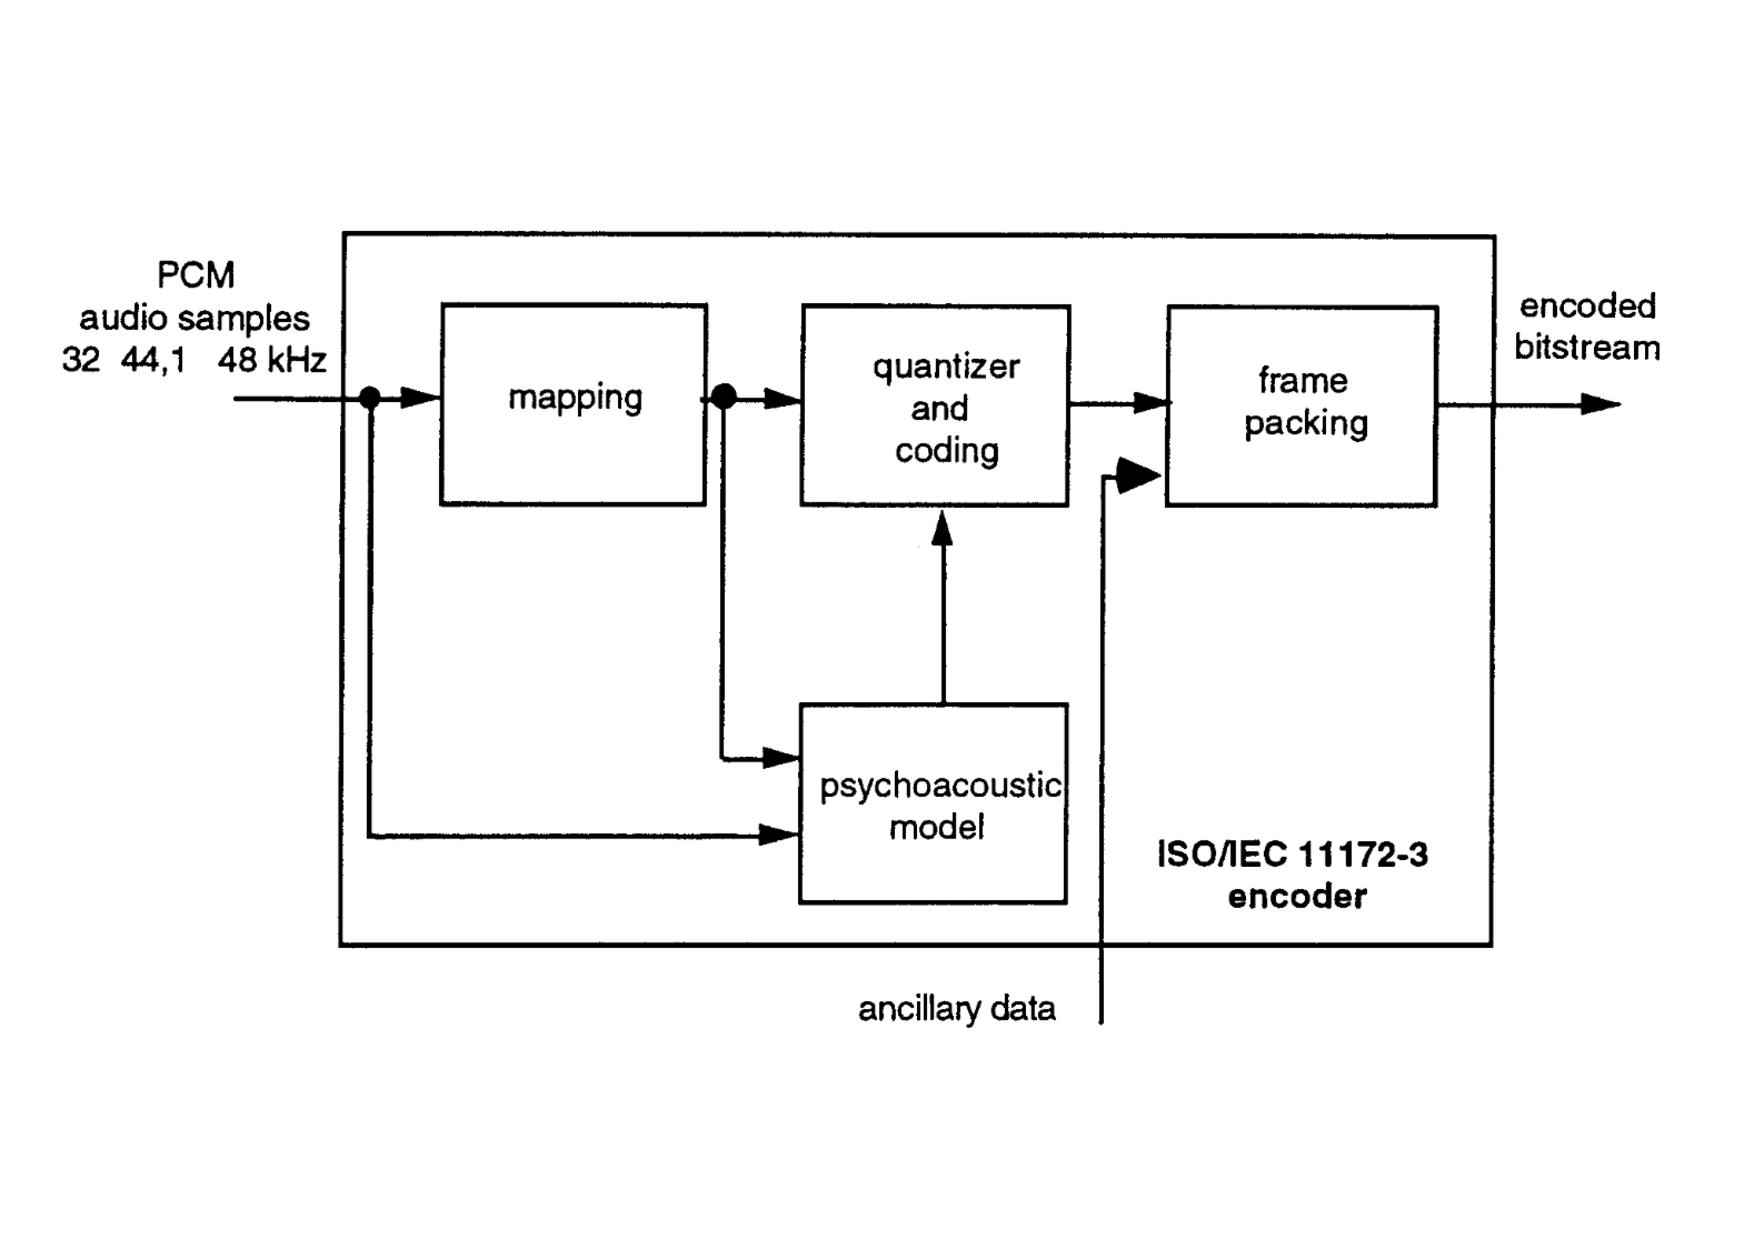
\includegraphics[width=0.85\linewidth]{encoder.pdf}}
\caption{Audio encoder basic structure.}
\label{fig:encoder}
\end{figure}

The encoding process contains four main blocks: \textit{mapping}, \textit{psychoacoustic model}, \textit{quantizer and coding}, and \textit{frame packing}.

First, the \textbf{mapping} block creates a filtered and subsampled representation of the input audio stream, usually called subband samples (for Layer II). At the same stage, the \textbf{psychoacoustic model} block creates a set of data to control the next block (\textit{quantizer and coding}). These control data depend on the coder implementation, with one possibility being the use of a masking threshold estimation.

Then, the \textbf{quantizer and coding} block creates a set of coding symbols from the mapped input samples, depending on the encoding system once again. 

Finally, the \textbf{frame packing} block assembles the actual bitstream from the output data of the previous blocks, adding information if necessary.

The encoding process supports four different modes: single channel, dual channel (two independent audio signals coded within one bitstream), stereo (left and right signals of a stereo pair coded within one bitstream), and Joint Stereo (with the stereo irrelevancy and redundancy exploited).

\subsubsection{Psychoacoustic encoder}

The ISO/IEC 11172-3 (MPEG-Audio) psychoacoustic algorithm contains four primary parts, as shown in figure \ref{fig:algorithm}: \textit{Filter Bank}, \textit{Psychoacoustic Model}, \textit{Bit or Noise Allocation} and \textit{Bitstream Formatting}~\cite{11172}.

%figure page 66 iso
\begin{figure}[H]
\centerline{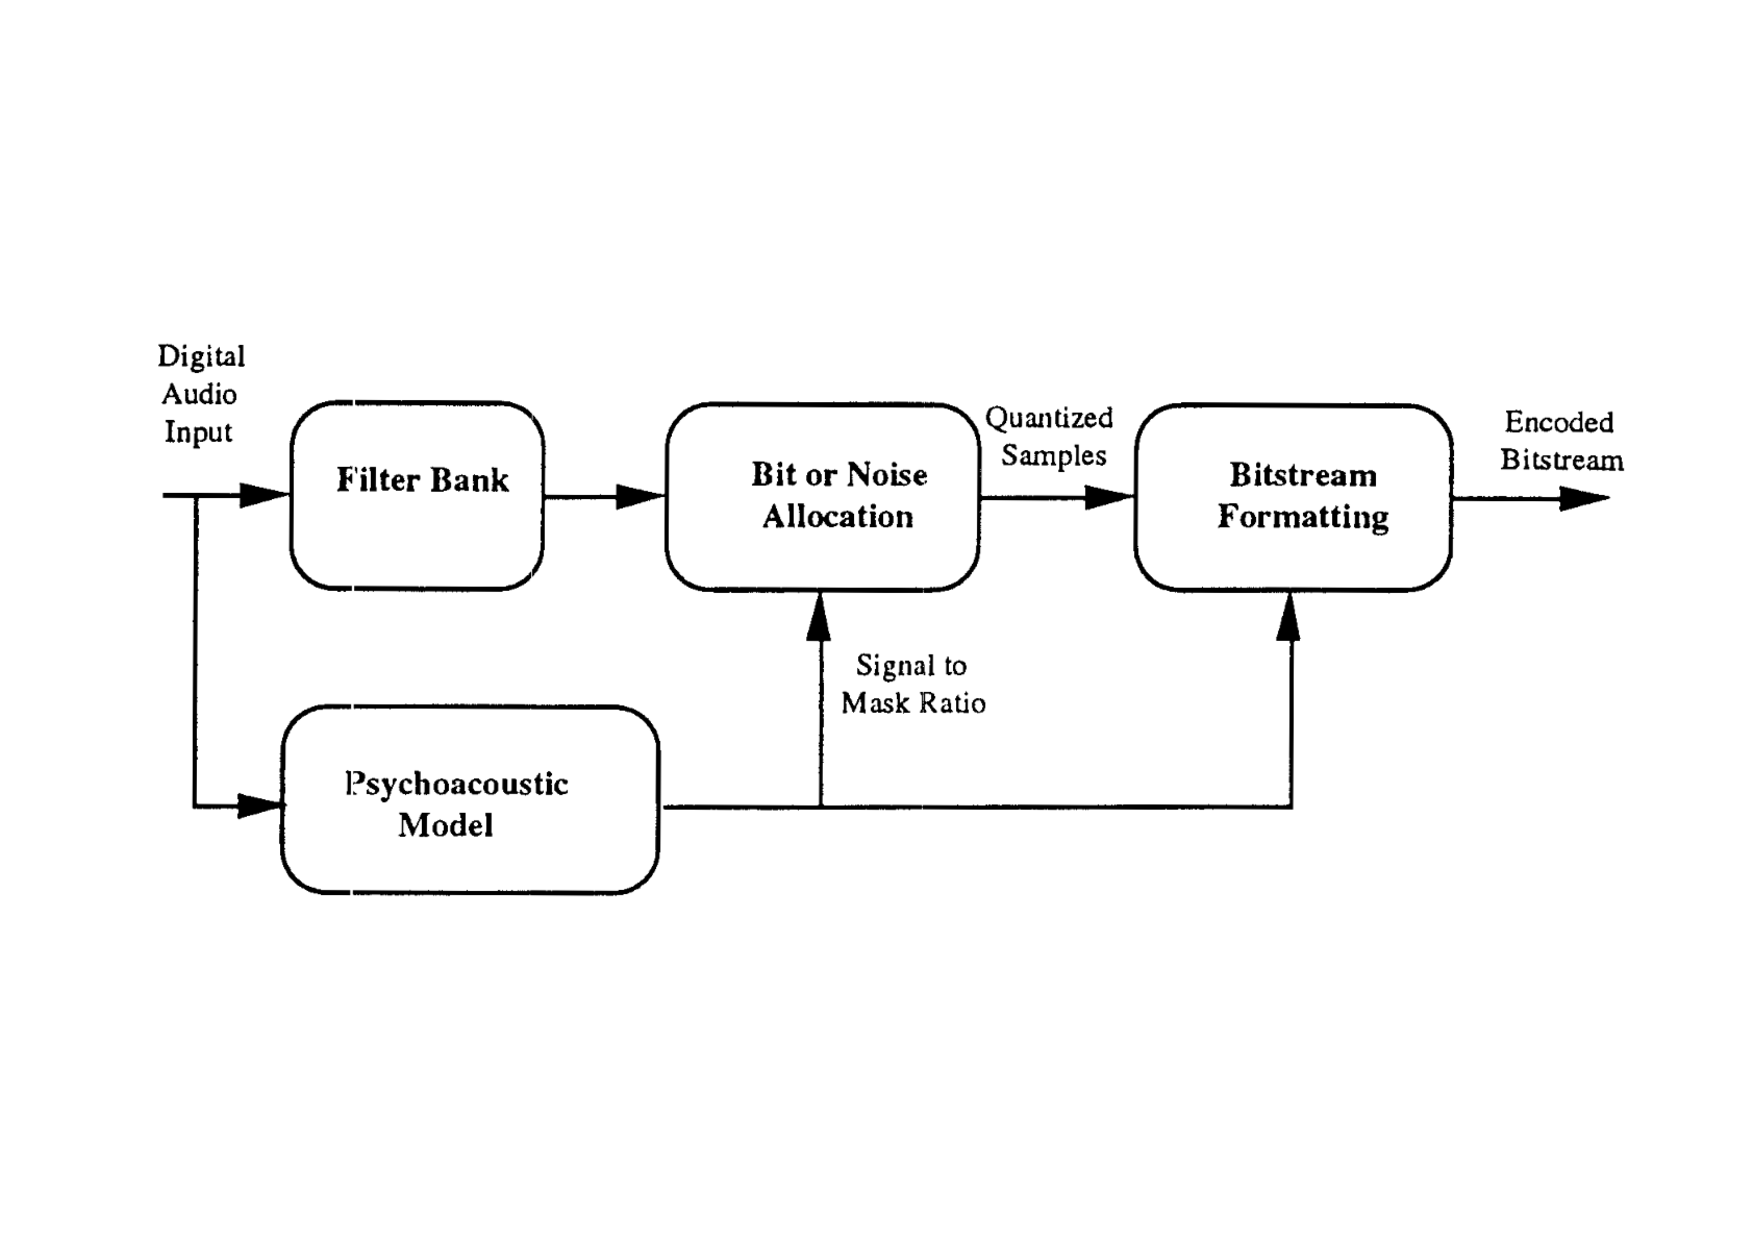
\includegraphics[width=0.85\linewidth]{iso-encoder.pdf}}
\caption{ISO/IEC 11172-3 encoder block diagram.}
\label{fig:algorithm}
\end{figure}

The \textbf{Filter Bank} does a time-to-frequency mapping, being one of two types. It can be a polyphase filter bank or a hybrid polyphase/Modified discrete cosine transform (MDCT)~\cite{mdct} filter bank, with each delivering a specific mapping in time and frequency.
These filterbanks are critically sampled, having the same number of samples in both analyzed and time domains, and provide the primary frequency separation for the encoder, with quantized output samples. 
In layer II, a filter bank with 32 subbands is used. In each subband, 12 or 36 samples are grouped for processing.

The \textbf{Psychoacoustic Model} calculates a just noticeable noise level for each band in the filter bank. This noise level is used in the \textit{Bit or Noise Allocation} part to determine the actual quantizers and quantizer levels. 
The final output of the model is a signal-to-mask ratio (SMR) for each band (Layer II).
%annex D  (MOdel 1 Layer II)

The \textbf{Bit or Noise Allocation} takes both the output samples from the \textit{Filter Bank} and the SMR from the \textit{Psychoacoustic Model} and adjusts the bit allocation, to meet the bitrate and masking requirements. At low bitrates, these methods attempt to spend bits in a way that is inoffensive when they cannot meet the psychoacoustic demand at the required bitrate.
In Layer II, this method is a bit allocation process, where several bits are assigned to each sample (or group of samples) in each subband.

The \textbf{Bitstream Formatting} takes the quantized filterbank outputs, together with the bit allocation and other required side information, and encodes and efficiently formats all that information. 
In Layer II, a fixed Pulse code modulation (PCM) code is used for each subband sample, with the exception that quantized samples may be grouped.

%figure page 79 iso
Figure \ref{fig:flow-encoder} shows a more detailed Layer II Encoder flow chart~\cite{11172}.

\begin{figure}[H]
\centerline{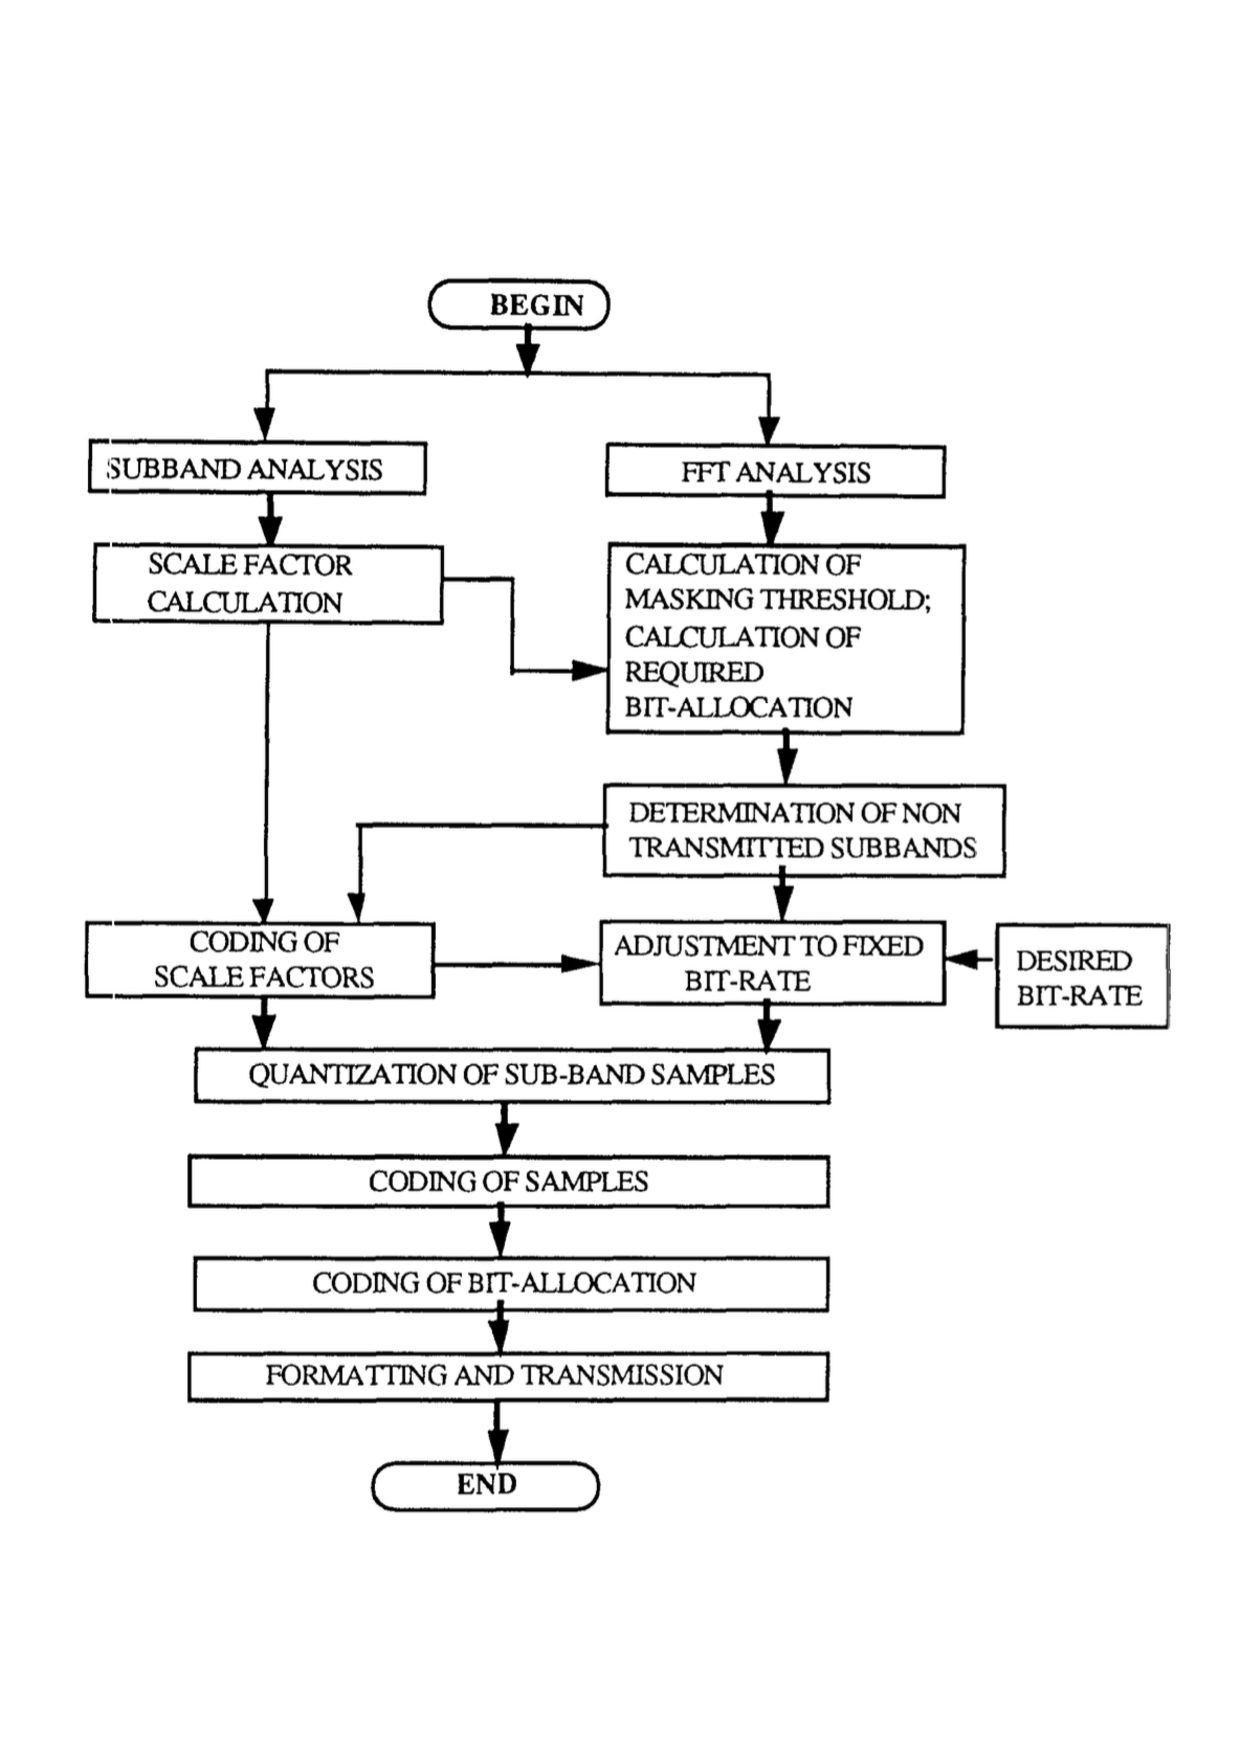
\includegraphics[width=0.70\linewidth]{flow-encoder.pdf}}
\caption{Layer II encoder flow chart.}
\label{fig:flow-encoder}
\end{figure}

\subsection{MPEG-1/2 Layers I/II}

The Moving Picture Experts Group (MPEG) is a working group that sets standards for media coding, established by the International Organization for Standardization (ISO)~\cite{iso} and the International Electrotechnical Commission (IEC)~\cite{iec}. Thus, the MPEG standard is a set of specifications for audio and video compression, containing two variations (among others), MPEG-1 and MPEG-2. Both variations cover audio and video, but since this work is focused on audio, the relevant standards are MPEG-1 Audio and MPEG-2 Audio.
%is a working group of ISO/IEC with the mission to develop standards for coded representation of digital audio and video and related data.

The MPEG-1 Audio, defined by ISO/IEC 11172-3~\cite{11172} (explained in the next section), standardizes the information that an audio encoder must produce to write a bitstream conformant with the standard requirements. Moreover, it standardizes how an audio decoder has to parse, decompress, and resynthesize the information to reconstruct the original audio stream.

This standard performs perceptual audio coding, which does not attempt to retain the input signal exactly after encoding and decoding. Instead, it ensures that the output signal sounds the same to a human listener. %, by eliminating the parts of the input signal that are irrelevant to the human ear 
More precisely, an MPEG-1 audio encoder transforms the sound signal into the frequency domain, eliminates the frequency components that are masked by stronger frequency components, and packages the analyzed signal into a compressed audio bitstream.

%working principle
Focusing on the encoding process, the primary psychoacoustic effect is called "auditory masking", where parts of a signal are not audible due to the function of the human auditory system. For example, if there is a sound that consists mainly of one frequency, all other sounds that consist of a close frequency but are much quieter will not be heard.  
%where exploiting the limitations of perception and removal of irrelevance is key to achieving a significant reduction in bitrate while preserving subjective audio quality.
Considering this, the parts of the signal that are masked are commonly called irrelevant, as opposed to the redundant parts that are removed. % by a lossless coding operation 
To eliminate this irrelevancy, the encoder contains a \textbf{psychoacoustic model} which analyzes the input signals within consecutive time blocks and determines, for each block, the spectral components of the input audio signal (by applying a \textbf{frequency transform}). Then, it models the masking properties of the human auditory system, and estimates the noise level for each frequency band, usually called "threshold of masking". 
In parallel, the input signal is fed through a time-to-frequency mapping, resulting in spectrum components for subsequent coding.  
Finally, in the \textbf{quantization and coding} stage, the encoder tries to allocate the available number of data bits, meeting both the bitrate and masking requirements ("threshold of masking"). The information on how the bits are distributed over the spectrum is contained in the bitstream as side information.

%layers
The MPEG-1 standardizes three different coding schemes, namely Layer I, Layer II, and Layer III, with the first two layers being the relevant ones in this work.
Layer I has the lowest complexity and is specifically suitable for applications where the encoder complexity plays an important role.
Layer II requires a more complex encoder and decoder, being directed towards one-to-many applications, i.e. one encoder serves many decoders. 

Compared to Layer I, Layer II can remove more of the signal redundancy and apply the psychoacoustic threshold more efficiently.
%bitstream
In Layer II, the digitized audio signal is divided into blocks of 1152 samples, with each block being encoded within one MPEG-1 audio frame.
Therefore, an MPEG-1 audio stream consists of consecutive audio frames, each one containing a header and the encoded data. The header contains general information, such as MPEG Layer, sampling frequency, number of channels, etc. Although most of this information may be the same for all frames, MPEG decided to give each audio frame a header to simplify synchronization and bitstream editing.

%MPEG-2
All the previous information describes one variation of MPEG, MPEG-1 Audio. This variation represents the first phase of dealing with mono and two-channel stereo sound coding, at sampling frequencies commonly used for high-quality audio (48, 44.1, and 32 kHz). 
In addition, there is a second variation, MPEG-2 Audio, which includes three main points.
The first point is the extension of MPEG-1 to lower sampling frequencies (16 kHz, 22.05 kHz, and 24 kHz), providing better sound quality at very low bit rates.
The second point is the backward-compatible (BC) extension of MPEG-1 to multichannel sound, supporting up to 5 full bandwidth channels plus one low-frequency enhancement channel. The MPEG-2 BC stream adheres to the structure of an MPEG-1 bitstream, meaning that an MPEG-2 BC stream can be read and interpreted by an MPEG-1 audio decoder.
The third and last point is a new coding scheme called Advanced Audio Coding (AAC), which is more efficient and presents higher quality.
 
%applications
Today, the MPEG-1 Audio standard is the most widely compatible lossy audio format in the world, thanks to technical merits and excellent audio quality performance.
Within the professional and consumer market, four fields of applications can be identified, namely broadcasting, storage, multimedia, and telecommunication. %This variety of applications is possible because of the wide range of bitrates and the numerous configurations allowed in MPEG-1.  
% What is the work? motivation?


\subsection{MPEG-1/2 Layers I/II IP cores}

Knowing the wide range of customers that need digital audio, belonging to all industries, this work proposes developing an IP core to encode MPEG-1/2 Layer II, using a RISC-V processor and hardware accelerators.
 
An intellectual property core (IP core) consists of a block of logic or data that is used in a semiconductor chip when making a field-programmable gate array (FPGA) or application-specific integrated circuit (ASIC)~\cite{fpga}.
Therefore, IP cores are usually the property of a particular person or company, being created throughout the design process and eventually turned into components for reuse. Third-party IPs can also be purchased and implemented into designs. 

Ideally, an IP core should be entirely portable, meaning it should be possible to insert it into any vendor technology or design methodology. However, this is not always the case, existing two main categories of IP cores, soft IP core, and hard IP core. 
A soft IP core is generally offered as a synthesizable RTL model. It is developed in a hardware description language like SystemVerilog~\cite{systemverilog} or VHSIC Hardware Description Language (VHDL)~\cite{vhdl}, or can occasionally be provided synthesized with a gate-level netlist. One advantage of this IP is the possibility to customize during the physical design phase and map to any process technology. 
A hard IP core has logic and physical implementation, meaning that its physical layout is finished and fixed in a particular process technology.
One advantage of this core is the better predictability of chip timing performance and area for its technology. 

A company that purchases an IP core license usually receives everything that's required to design, test, and implement the core in its product. It may also receive logic and test patterns, signal specifications, design notes, and a list of known bugs or limitations.

%introduction for the examples
Two IP Cores, two Chips, and one Software that perform MPEG-1/2 Layer I/II audio encoding are presented in the following subsections.

\subsubsection{CWda74 MPEG-1/2 – Layer I/II Audio Encoder}
 
The \textit{CWda74}~\cite{CWda74} is an audio IP core capable of encoding one audio stream in real-time, provided by \textit{Coreworks, S.A.}~\cite{coreworks}.

This IP core contains the MPEG-1/2 Layer I/II encoder software and the \textit{Coreworks} processor-based hardware audio engine platform (\textit{CWda1011}). 
Initially, the software is compiled into a binary file, which can be automatically boot-loaded through one of the control interfaces, parallel Advanced Microcontroller Bus Architecture (AMBA)~\cite{bib:axi_amba} Advanced Peripheral Bus (APB) or serial Serial Peripheral Interface (SPI). 
Once the software is loaded, the program runs on the audio engine platform. The system can be configured, controlled, and monitored through a configuration, control, and status register file, accessed by the control interfaces.  
The Audio Input and Output Interfaces use a native parallel interface. Other standard audio interfaces, such as Inter-IC Sound (I2S)/Time Division Multiplexed (TDM) and Sony/Philips Digital Interface (SPDIF), are also available.
The Memory Interface can be AMBA Advanced eXtensible Interface (AXI) (for ASIC or Xilinx FPGA), Avalon (for Altera~\cite{bib:intel} FPGA), or Memory Interface Generator (MIG) (for Xilinx FPGA).

The \textit{CWda74} IP core delivers Program binary, Software manual, Netlist or RTL, Implementation constraints, and Hardware datasheet. 
As attributes, it presents low operation frequency and low power consumption, with the possibility of being optimized to fulfill different design specifications.
Table~\ref{tab:coreworks} describes the main features.

\vspace{0.5cm}

\begin{table}[H]
    \centering
    \begin{tabular}{|c|}
        \hline
        \textbf{Features} \\
        \hline
         ISO/IEC 11172-3 and 13818-3 standards \\
         \hline
         Fraunhofer IIS high-quality software\\
         \hline
         Mono, dual mono, stereo, and joint stereo channel modes \\
         \hline
         16, 22.05, 24, 32, 44.1, and 48 kHz sampling rates \\
         \hline
         16 to 24-bit input audio resolution \\
         \hline
         300 kB external memory requirement\\
         \hline
         Configurable output latency \\
         \hline
         1 frame minimum latency\\
         \hline
         Control, configuration, and monitoring protocol \\
         \hline
         Real-time operation @75 MHz \\
         \hline
    \end{tabular}
    \caption{\textit{CWda74} features.}
    \label{tab:coreworks}
\end{table}

\vspace{0.3cm}

\subsubsection{IPB-MPEG-SE MPEG-1/2 – Layer I/II Audio Encoder}

The \textit{IPB-MPEG-SE}~\cite{ipb-mpeg-se} is an audio IP core capable of encoding up to two stereo audio streams in real-time, provided by \textit{IPbloq}~\cite{bib:ipbloq}.

This IP core is designed to run on the \textit{IPbloq} audio engine platform \textit{IPB-PLAT}, which supports the encoding and decoding of multiple streams in multiple formats, on a single device. More precisely, the \textit{IPB-MPEG-SE} software requires an instance of the \textit{IPB-PLAT} audio engine platform with only one processor. 

Initially, the program is uploaded using a hardware interface. Then, the system is configured, run, and monitored through a configuration, control, and status register file, accessed by the same Control Interface.
The Audio Input and Output Interfaces include a native parallel interface. Other interfaces, such as I2S/TDM and SPDIF/Audio Engineering Society 3 (AES3), are also available.

The \textit{IPB-MPEG-SE} IP core delivers Program binary, Software manual, RTL of FPGA netlist, Implementation constraints, and Hardware datasheet. 
As attributes, it presents low operation frequency, low power consumption, and compact hardware implementation, fitting economically in FPGAs and ASICs.
In terms of features, this IP core is very similar to the \textit{CWda74}, extending the Real-time operation for two audio streams @150 MHz. 

%\vspace{0.2cm}

\subsection{MPEG-1/2 Layers I/II Chips}

\subsubsection{CX23415 MPEG-2 Codec}

The \textit{CX23415}~\cite{cx23415} is a low-cost, full-duplex MPEG-2 codec that integrates the functionality of several Integrated Circuits (ICs) in a single device, provided by \textit{Conexant Systems, Inc}~\cite{bib:conexant}.

This chip was the first device to deliver MPEG-2 audio/video encoding and decoding, transport stream (TS) generation, and on-screen display control in a single chip. The ability to incorporate up to five different chip functionalities allowed for reducing the cost of designing and manufacturing digital audio and video products.

%As attributes, the CX23415 presents prefiltering improvements, including built-in linear filters that dynamically change or soften images in the pre-processing stage. As a result, users obtain the best possible picture, even as the data rate is reduced and the recording time is lengthened. Other video quality improvements included an increased motion search range, the decoupling of motion estimation from encoders, and an adaptive quantization scheme. 

%The CX23415 incorporates an OSD for graphics control and advanced GUI acceleration to support user interfaces and the display containing broadcast and service information from electronic program guides. The controller includes a BITBLT acceleration engine and Deflicker filter, supporting a variety of pixel formats, including an 8-bit color index and 32-bit RGBA 8:8:8:8.

For audio encoding and decoding, the \textit{CX23415} integrates MPEG-1 Layer II, with sampling rates of 32 kHz, 44.1 kHz, and 48 kHz, and compressed bit rates up to 448 kbit/sec. The encoder supports 16-bit samples, while the decoder supports 16-, 18-, or 20-bit outputs.

As audio input and output, this chip supports Stereo Sony I2S. As MPEG input and output, it supports Peripheral Component Interconnect Direct memory access (PCI DMA) master or PCI slave, 8-bit parallel program data, 8-bit parallel SPI transport data, and 1-bit serial transport data.

The \textit{CX23415} most relevant features are high-quality real-time encoding and MPEG-1 and MPEG-2 support.

\subsubsection{Futura II ASI+IP™}

The \textit{Futura II}~\cite{futura} is a broadcast-oriented MPEG-2/H.264 encoder that supports all standard broadcast formats, including North American standards. 

%delivers MPEG-2 video at bit rates of 3.4 to 19.39 Mbps and H.264 video at 2.5 to 19.39 Mbps.
This device, developed by \textit{Magnum Semiconductor Inc.}, is capable of encoding MPEG-1 Layer II at 192, 224, 256, 320, and 384 Kbps, with sampling rates of 32, 44.1, and 48 kHz. It can also encode Dolby Digital-3 (AC-3), MPEG-4 Advanced Audio Codec – Low Complexity (AAC-LC), and High-Efficiency Advanced Audio Coding (HE-AAC).

As analog audio input, it supports one Stereo (two channels) with a frequency range from 20Hz to 20KHz. As digital audio input, it supports the Audio Engineering Society-European Broadcasting Union (AES-EBU) and Serial digital interface/High-Definition Multimedia Interface (SDI/HDMI) (H.264 only).
As output, both ASI and IP ports deliver MPEG-2 with a bit rate from 3.4 to 19.39 Mbps.

The \textit{Futura II}'s most relevant features are 800 milliseconds latency, user-selectable resolution and bit rate, and two encoding modes, Constant Bit Rate (CBR) and Variable Bitrate (VBR).

\subsection{MPEG-1/2 Layers I/II Systems}

\subsubsection{MPEG-2 Encoder CW-4888}

The \textit{CW-4888}~\cite{cw4888} is an MPEG-2 encoder that feeds video signals of analog program sources, like cameras and broadcasters, to digital broadcast networks.

Initially, this device receives the standard composite video and the associated sound signals. Then, it digitizes and compresses the input according to the MPEG-2 standard, outputting the result as Asynchronous Serial Interface (ASI)~\cite{asi} or Internet Protocol (IP)~\cite{ip} streams.

For audio, this device supports mono, dual, stereo, and joint stereo sound modes. The audio input signal is converted by a dual-channel encoder, which performs MPEG-1 layer I/II compression based on ISO/IEC 11172-3~\cite{11172}. 
The bit rate can be set between 32 and 448 kbit/s, with sampling frequencies of 33 kHz, 44.1 kHz, and 48 kHz.

The \textit{CW-4888}'s most relevant features are FPGA circuitry and the option for two or four independent encoder units in one frame.
As attributes, it presents extremely low power consumption, high reliability, and a long lifespan.

\subsection{MPEG-1/2 Layers I/II Software}

\subsubsection{TooLAME/LAME}

The \textit{LAME}~\cite{bib:lame} is a high-quality MPEG Layer III audio encoder, licensed under the Lesser General Public License (LGPL)~\cite{lgpl} and considered the best MP3 encoding software at mid-high and variable bitrates. 
As attributes, this software delivers better quality compared to all other encoders at most bitrates, better quality and speed compared to ISO reference software, and three different encoding modes (CBR, VBR, and Average Bit Rate (ABR)). This encoder is also free format and compilable as a shared library (on Linux/Unix) and Dynamic link library (DLL)~\cite{dll} (on Windows).

Based on portions of \textit{LAME} and ISO dist10 code, the \textit{TooLAME}~\cite{bib:toolame} was developed as a free software MPEG-1 Layer II audio encoder, written primarily by Mike Cheng. \textit{TooLAME} became well-known and widely used for its particularly high audio quality, despite the existence of many MP2 encoders.

\subsubsection{TwoLAME}

Despite being unmaintained since 2003, the \textit{TooLAME} software was directly succeeded by the \textit{TwoLAME}~\cite{bib:twolame} code fork, which is the focus of this work.
Thus, \textit{TwoLAME} is an optimized MPEG Layer 2 audio encoder, based on \textit{TooLAME}, with its latest version (0.4) released in 2019. 
Table~\ref{tab:twolame} describes the additional features not provided in the original \textit{TooLAME}.

\vspace{0.5cm}

\begin{table}[H]
    \centering
    \begin{tabular}{|c|}
        \hline
        \textbf{Features} \\
        \hline
         Static and shared library (\textit{libtwolame}) \\
         \hline
         Fully thread-safe\\
         \hline
         API similar to \textit{LAME}'s (easy porting) \\
         \hline
         Front-end supports a wider range of input files \\
         \hline
         \textit{automake}/\textit{libtool}/\textit{pkgconfig} based build system \\
         \hline
         Written in Standard C (ISO C99 compliant)\\
         \hline
    \end{tabular}
    \caption{\textit{TwoLAME} features.}
    \label{tab:twolame}
\end{table}

The \textit{TwoLAME} repository includes a \textit{simplefrontend} directory that contains a basic implementation of the software, written in C.
It has a \textit{simplefrontend.c} file, containing the \textit{main()} function, and two other files, \textit{audio\_wave.c} and \textit{audio\_wave.h}.
Figure \ref{pseudo1} shows the pseudo code for the first part of \textit{simplefrontend.c}, mainly consisting of initialization.

\begin{figure}[H]
\centerline{\fbox{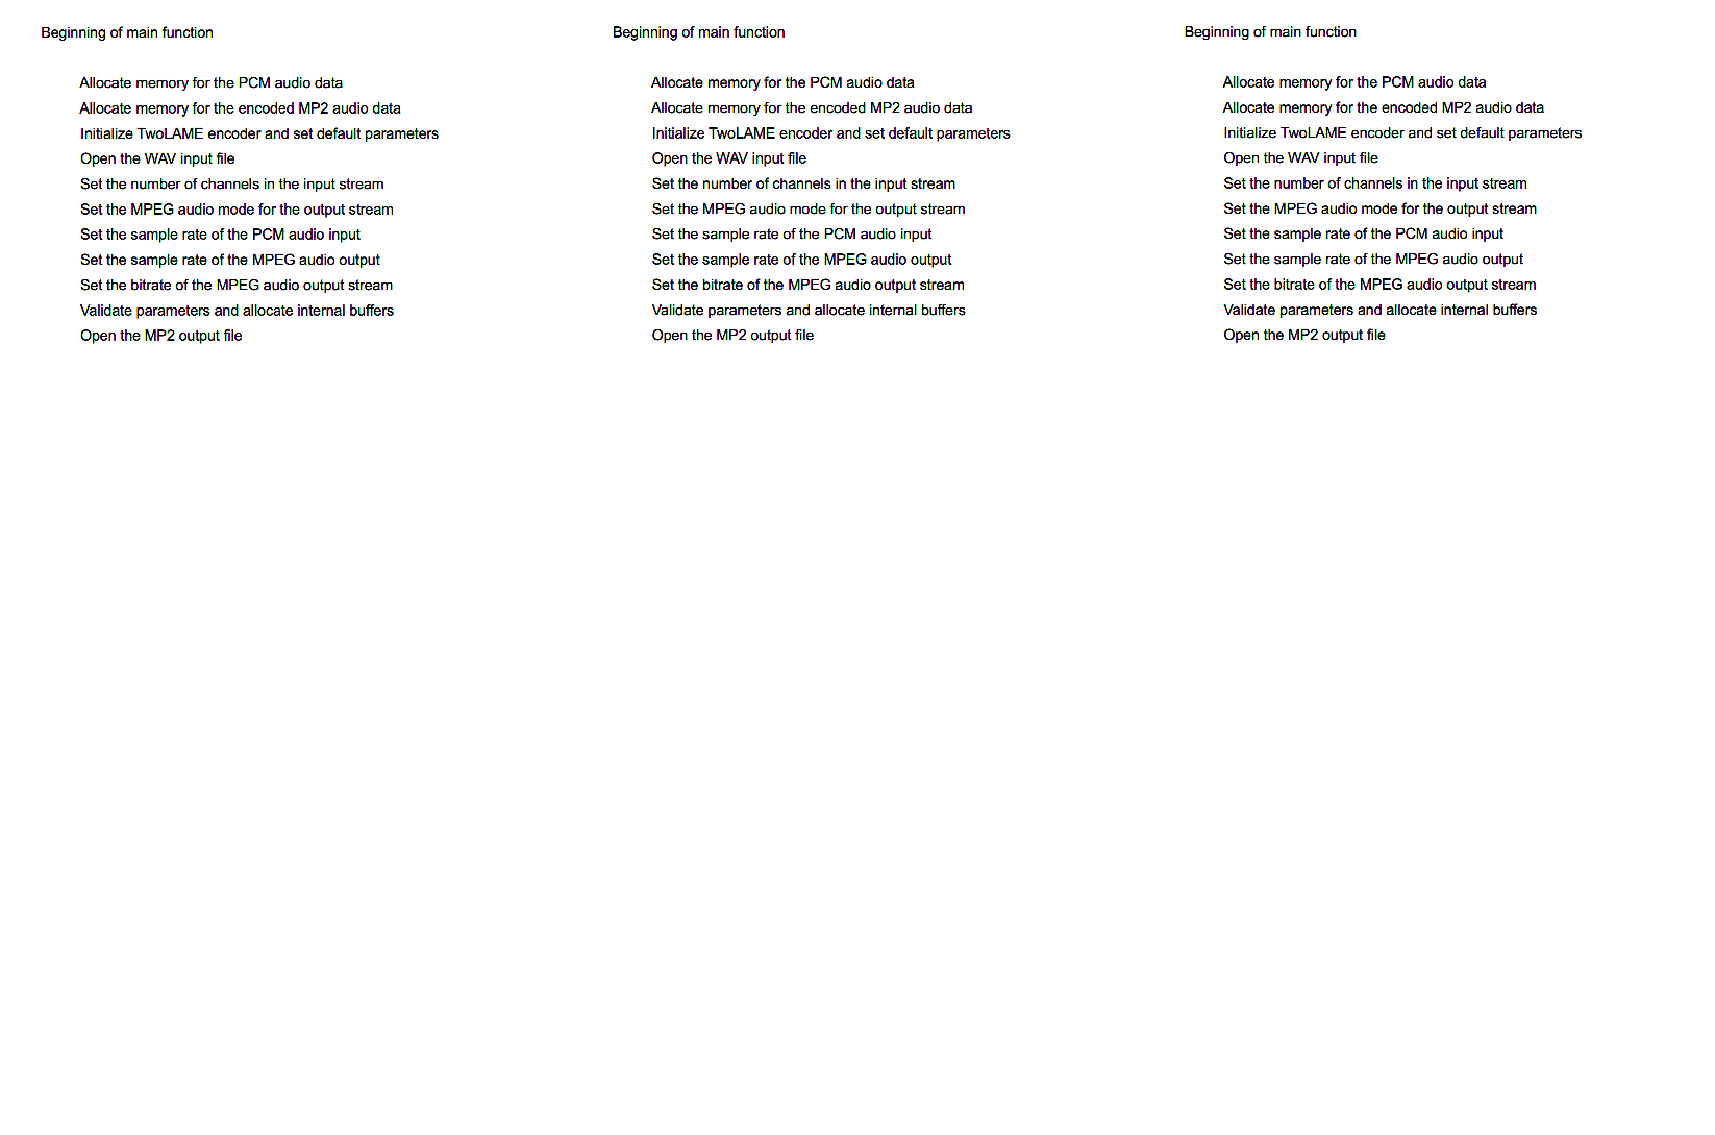
\includegraphics[width=0.80\linewidth]{pseudo1.pdf}}}
\caption{First part of \textit{firmware.c} pseudo code.}
\label{pseudo1}
\end{figure}

%\vspace{1cm}

The program starts by allocating memory for two different buffers to allow the encoding process. One of them is \textit{pcmaudio}, which receives part of the original input file. This PCM buffer has a size of AUDIOBUFSIZE multiplied by two (corresponds to the number of bytes of short integer type), being allocated and initialized with zero by \textit{calloc}. The other buffer is \textit{mp2buffer}, which receives part of the encoded file that is later written in the output file. This MP2 buffer has a size of MP2BUFSIZE (corresponds to the number of bytes of unsigned char type), being allocated and initialized with zero by \textit{calloc} as well.

Then comes the \textit{TwoLAME}-related stuff. The first function is \textit{twolame\_init}, which initializes the encoding software by setting defaults for all parameters and returning a pointer necessary to all future \textit{TwoLAME} calls~\cite{bib:twolameapi}. The second function is \textit{wave\_init}, which parses the wave header. This function belongs to \textit{audio\_wave.c} and is responsible for processing the wave header (the first four bytes). Apart from identifying the file as WAVE, the header gives relevant information like sample rate and audio mode, which is collected in a \textit{wave\_info\_t} struct.
The remaining initialization functions specify encoding options. There is the \textit{twolame\_set\_num\_channels}, which sets the number of channels in the input stream. There is also the \textit{twolame\_set\_mode}, which sets the MPEG Audio Mode (like mono or stereo) for the output stream. In addition, the \textit{twolame\_set\_in\_samplerate} sets the sample rate of the PCM audio input, while the \textit{twolame\_set\_out\_samplerate} sets the sample rate of the MPEG audio output. The \textit{twolame\_set\_bitrate} sets the bitrate of the MPEG audio output stream.

After defining the main encoding options, \textit{twolame\_init\_params} function is called. It prepares \textit{TwoLAME} to start encoding by checking all the parameters, making sure they are valid as well as allocating buffers and initializing internally used variables. Then, \textit{fopen} opens the output file where the encoded MP2 data is later written.

Moving to the \textit{TwoLAME} execution, figure \ref{pseudo2} shows the pseudo code for the second part of \textit{simplefrontend.c}, mainly consisting of the encoding process.

\begin{figure}[H]
\centerline{\fbox{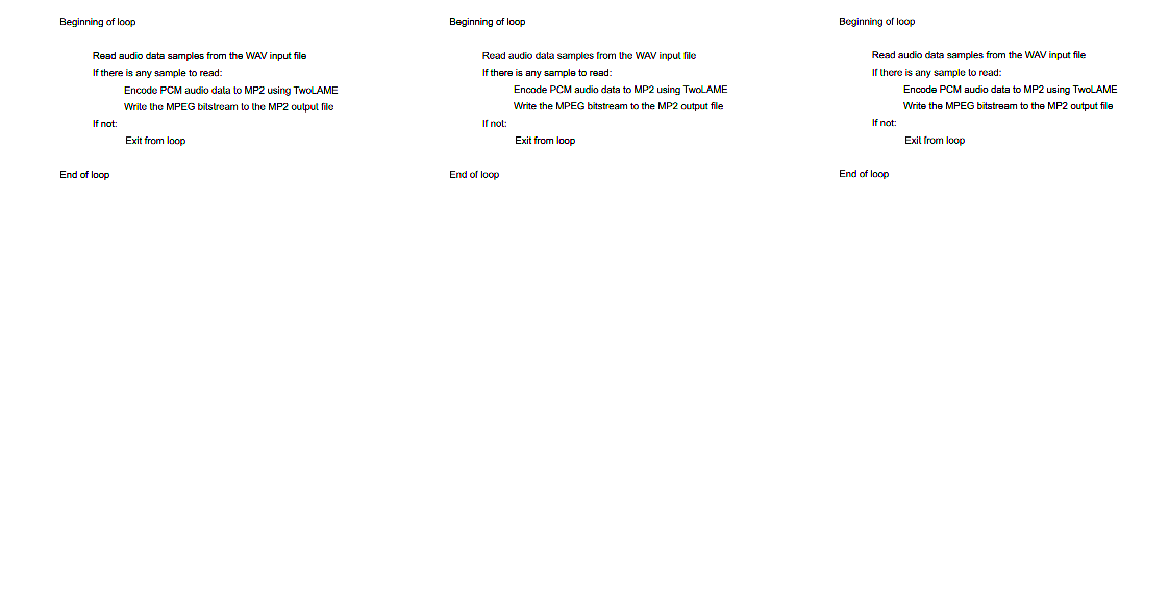
\includegraphics[width=0.80\linewidth]{pseudo2.pdf}}}
\caption{Second part of \textit{firmware.c} pseudo code.}
\label{pseudo2}
\end{figure}

%\vspace{1cm}

This process is based on a \textit{while} loop, as the main idea is to encode one part of the input audio file at a time, repeating the loop as many times as required. Therefore, each loop iteration starts by reading a chunk of audio data from the input WAV file through \textit{wave\_get\_samples}. This function also belongs to \textit{audio\_wave.c} and is responsible for reading AUDIOBUFSIZE samples to the PCM buffer (\textit{pcmaudio}). 
With the buffer already loaded, \textit{twolame\_encode\_buffer\_interleaved} is responsible for encoding the audio data using TwoLAME~\cite{bib:twolameapi}. This function has a high level of complexity, as expected. It makes use of the \textit{libtwolame} library, which englobes many processes. In particular, the function is composed by \textit{twolame\_buffer\_init}, which sets the \textit{bit\_stream} struct, and \textit{encode\_frame}, which encodes one audio frame at a time.
After being encoded, the chunk of data is written in the output file through \textit{fwrite}. The \textit{frames} variable, which counts the number of frames encoded, is also updated.  

Lastly, figure \ref{pseudo3} shows the pseudo code for the third part of \textit{simplefrontend.c}. 

\begin{figure}[H]
\centerline{\fbox{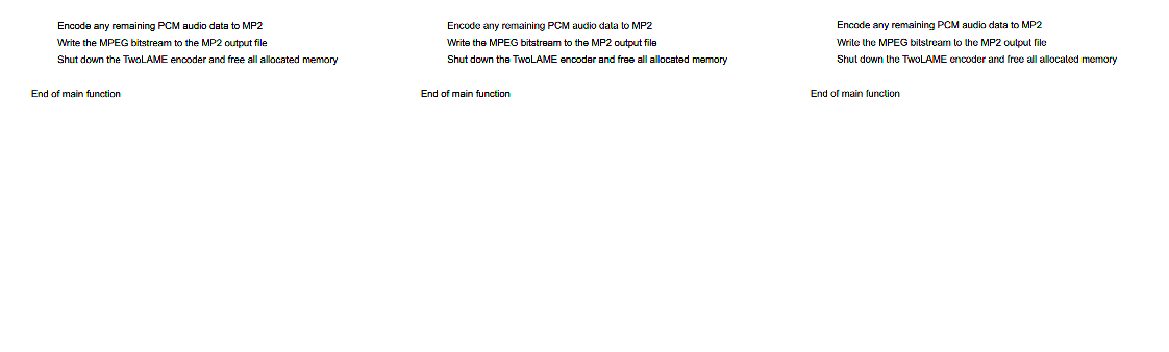
\includegraphics[width=0.80\linewidth]{pseudo3.pdf}}}
\caption{Third part of \textit{firmware.c} pseudo code.}
\label{pseudo3}
\end{figure}

%\vspace{1cm}

In this part, the \textit{TwoLAME} software finishes execution and so does the IOb-SoC system.
The first function is \textit{twolame\_encode\_flush}, which encodes any remaining buffered PCM audio, i.e., any remaining audio samples in the PCM buffer~\cite{bib:twolameapi}. This function is simpler than \textit{twolame\_encode\_buffer\_interleaved} and returns at most a single frame.
The \textit{fwrite} is used once again to write the remaining encoded data in the output file. Lastly, the encoding software is closed through \textit{twolame\_close} function. It shuts down the \textit{TwoLAME} encoder and frees all memory that was previously allocated, including PCM and MP2 buffers.

%%%%%%%%%%%%%%%%%%%%%%%%%%%%%%%%%%%%%%%%%%%%%%%%%%%%%%%%%%%%%%
    %current.tex below
%%%%%%%%%%%%%%%%%%%%%%%%%%%%%%%%%%%%%%%%%%%%%%%%%%%%%%%%%%%%%%

%Definição e proposta de metodologias a usar, com vista à consecução dos objetivos da Dissertação
%Resultados esperados e eventuais resultados preliminares

\subsection{System-on-Chip}
A System-on-Chip (SoC) is an integrated circuit that combines components of an electronic system. These components usually include a Central Processing Unit (CPU), memory interfaces, on-chip input/output devices, input/output interfaces, and secondary storage interfaces. 
Putting many elements of a computer system on a single piece of silicon has some advantages, such as low power requirements, reduced cost, increased performance, and reduced physical size.

%iob-soc (%components, FPGA resources, repository, accelerators)
The IOb-SoC is a System-on-Chip template, comprising an open-source RISC-V~\cite{riscv} processor, which users can modify, simulate, and implement in ASICs~\cite{asic} and FPGAs~\cite{fpga}.
This SoC, provided by \textit{IObundle, Lda}, supports stand-alone and boot-loading modes. It also allows an internal RAM~\cite{ram} or an external Double Data Rate (DDR)~\cite{ddr} controller via an L1/L2 cache system. 

Figure \ref{fig:iob} shows a base IOb-SoC high-level block diagram~\cite{iobsoc2022}.

\vspace{0.1cm}

\begin{figure}[H]
\centerline{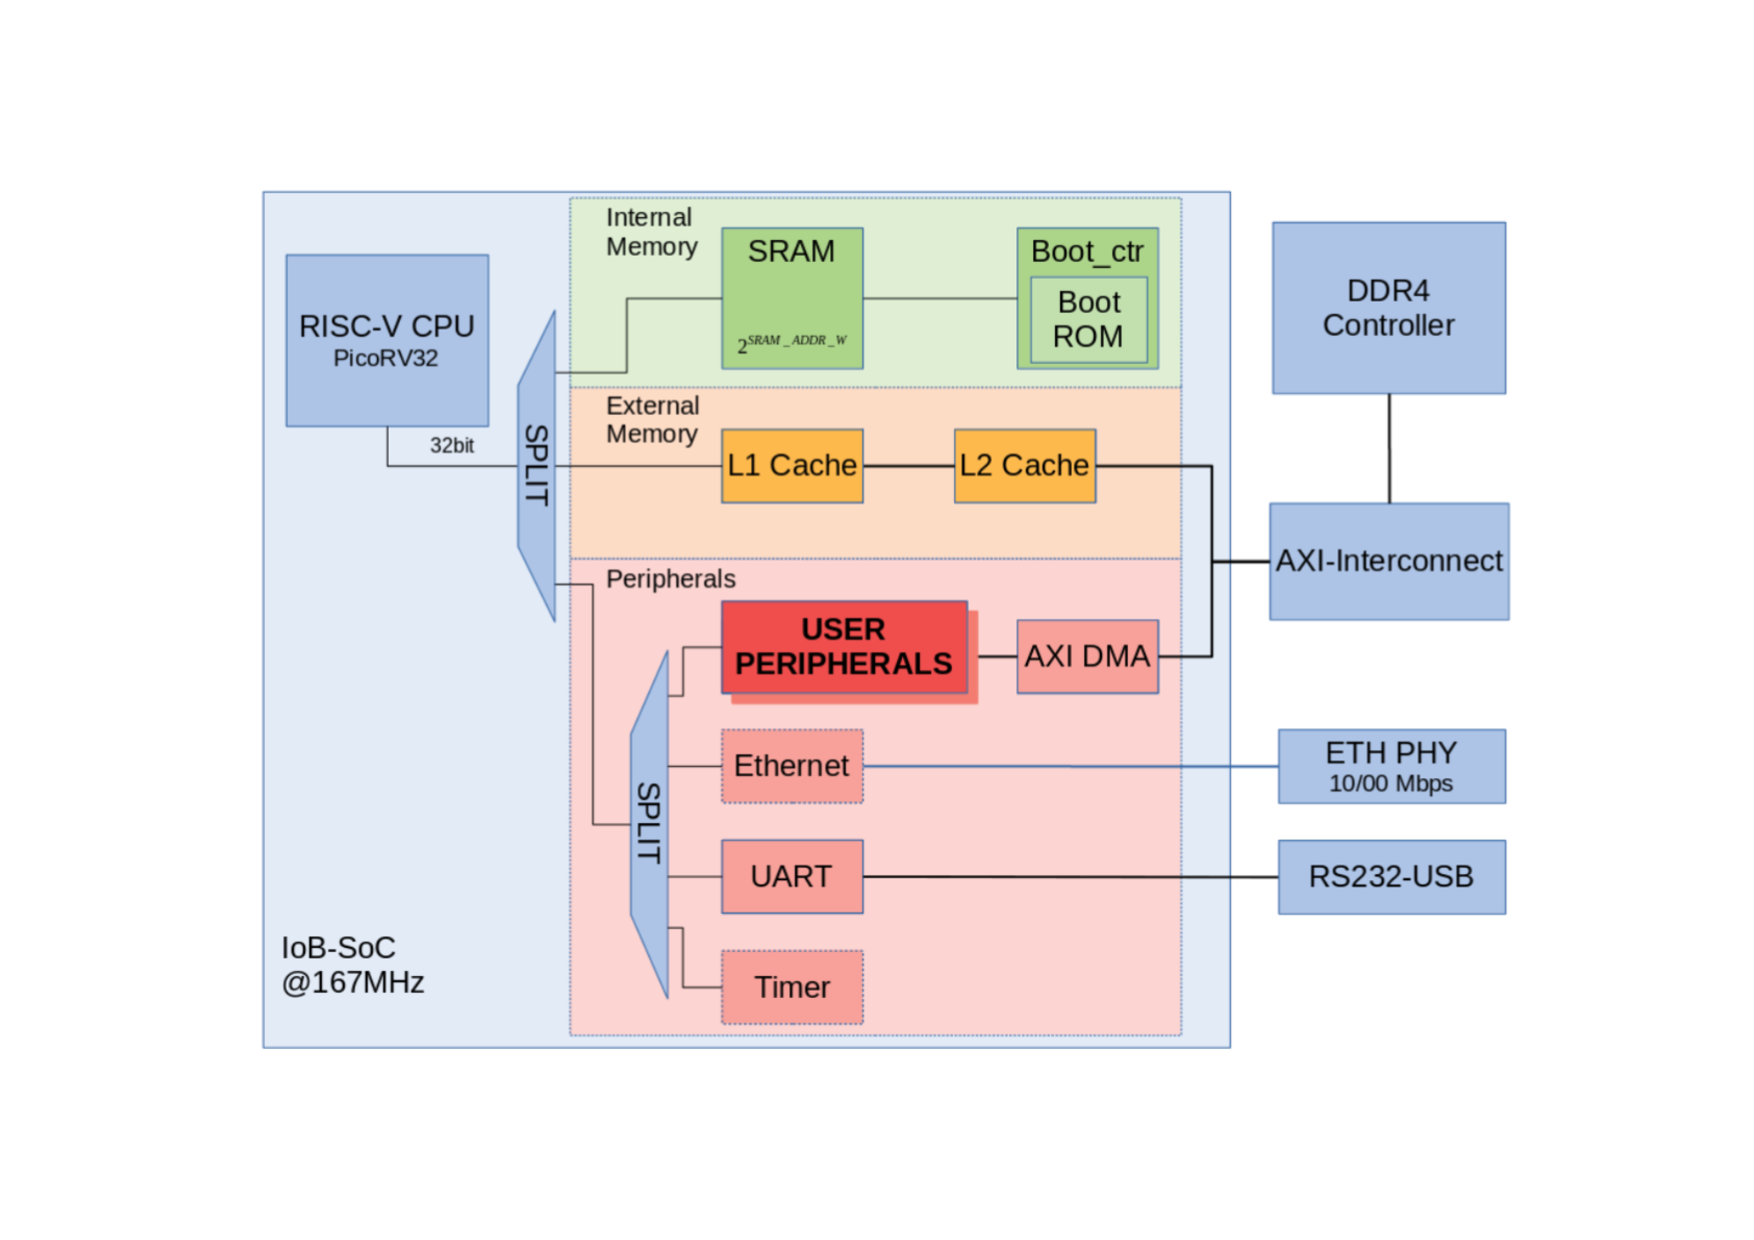
\includegraphics[width=0.85\linewidth]{iob-soc.pdf}}
\caption{Base IOb-SoC high-level block diagram.}
\label{fig:iob}
\end{figure}

\subsubsection{IOb-SoC components}
Starting with the \textbf{CPU}, the IOb-SoC uses a PicoRV32 CPU core, an open-source 32-bit processor that implements the RV32IMC instruction set, with an operating frequency of 167MHz.

As \textbf{Memory} subsystem, this SoC includes three main components. The Boot Read-Only Memory \textbf{Boot ROM} is a ROM used for booting the system. The Static Random Access Memory \textbf{SRAM}~\cite{sram} is an internal memory that allows the system to run the program or the bootloader without the need for external memory. The \textbf{Cache} is an optional component that stores data from the external Double Data Rate (DDR) memory.

The communication between the CPU and the system’s components (master and slaves) occurs through two buses. The \textbf{Memory bus} allows the CPU to communicate with the memory subsystem, while the \textbf{Peripheral bus} allows the CPU to communicate with system peripherals.

In addition, the \textbf{IOb-Interconnect} component is a bus switch responsible for the valid-ready handshake protocol between the CPU and all the peripherals. Based on the peripheral prefix from the address bus, this component selects which peripheral-specific bus connects to the CPU bus.  
The \textbf{IOb-Interconnect} multiplexes or demultiplexes, depending on the direction, the CPU bus signals (\textit{valid}, \textit{ready} and \textit{rdata}). By doing so, the component creates enough signals to ensure that there is one of each signal for each of the peripherals. Optionally, two peripherals connected to the peripheral bus can communicate directly without CPU intervention, allowing for faster data transfers between peripherals.

There is also a \textbf{Native to AXI adapter}, which allows communication between peripherals and memory controllers that use the AXI4~\cite{bib:axi_amba} protocol. Since the CPU only contains the native bus, the IOb-SoC uses this component to convert the signals from one bus to the other, with each peripheral that uses the AXI4-Lite port containing one \textbf{Native to AXI adapter}.

Finally, The Universal Asynchronous Receiver-Transmitter (\textbf{\textbf{UART}}) peripheral allows the SoC to communicate with external systems, through the RS-232 serial communication protocol.

All these components are integrated into IOb-SoC as GitHub submodules. They belong to repositories tracked by GitHub and forked from \textit{IObundle, Lda}, but arranged in a different way and with specific names.

\subsubsection{IOb-SoC deliverables and FPGA resources}
As deliverables, the IOb-SoC includes Hardware Description Language (HDL) source code, software C source code, simulation testbench, implementation constraints for map, place, and route, demo files, and user documentation for system integration.

Tables~\ref{tab:resorucesxilinx} and~\ref{tab:resorucescyclone} show the implementation resources used for \textit{Xilinx Kintex Ultrascale Devices} and \textit{Intel Cyclone V Devices}, respectively, according to the product brief.

\vspace{0.8cm}

\begin{table}[H]
\parbox{.45\linewidth}{
\centering
\begin{tabular}{|c|c|c|}
        \hline
         \textbf{Resource} & \textbf{Usage}  \\
         \hline
         LUTs & 1869 \\
         \hline
         Registers & 1029 \\
         \hline
         DSPs & 4 \\
         \hline
         BRAM & 5 \\
         \hline
         PIN & 6 \\
         \hline
\end{tabular}
\caption{Implementation resources for \textit{Xilinx Kintex
Ultrascale} Devices.}
\label{tab:resorucesxilinx}
}
\hfill
\parbox{.45\linewidth}{
\centering
\begin{tabular}{|c|c|c|}
        \hline
         \textbf{Resource} & \textbf{Usage}  \\
         \hline
         ALM & 1335 \\
         \hline
         FF & 1177 \\
         \hline
         DSP & 3 \\
         \hline
         BRAM blocks & 22 \\
         \hline
         BRAM bits & 165,888 \\
         \hline
         PIN & 6 \\
         \hline
\end{tabular}
\caption{Implementation resources for Intel Cyclone
V Devices.}
\label{tab:resorucescyclone}
}
\end{table}

%If the external memory interface is selected, an instruction L1 cache, a data L1 cache, and a shared L2 cache are added to the system. The L2 cache communicates with a 3rd party memory controller IP (typically a DDR controller) using an AXI4 master bus.

\subsubsection{IOb-SoC repository}

%peripherals
%simulators and FPGA
The IOb-SoC \textit{GitHub} repository is composed of specific directories and segments (Tool Command Language (TCL), Verilog, Makefile, etc), as briefly described in the list below.

\textbf{document/} This directory supports all the documentation, from LaTeX code and scripts to generated PDFs, like the guide and product brief.

\textbf{hardware/} This directory supports the hardware layer, containing multiple subdirectories.

\hspace{0.5cm} – \textbf{hardware.mk} This makefile contains targets, dependencies, and rules related to hardware.

\hspace{0.5cm} – \textbf{fpga/} This directory contains scripts to synthesize and run the system in FPGAs.

\hspace{1.2cm}\textbf{fpga.mk} This makefile contains targets, dependencies, and rules related to FPGAs.

\hspace{0.5cm} – \textbf{simulation/} This directory contains scripts to run RTL simulation in simulators.

\hspace{1.2cm}\textbf{simulation.mk} This makefile contains targets, dependencies, and rules related to simulators.

\hspace{0.5cm}– \textbf{src/} This directory contains Verilog scripts related to the system’s components.

\textbf{software/} This directory supports the software layer, containing multiple subdirectories.

\hspace{0.5cm}– \textbf{software.mk} This makefile contains targets, dependencies, and rules related to software.

\hspace{0.5cm}– \textbf{firmware/} This directory contains the software to run in the system, after initialization.

\hspace{0.5cm}– \textbf{bootloader/} This directory contains the bootable software for the system.

\hspace{0.5cm}– \textbf{pc-emul/} This directory contains scripts to run the firmware on the computer.

\hspace{0.5cm}– \textbf{console/} This directory contains the software that allows interaction between computer and FPGA, via UART.

\textbf{submodules/} This directory contains all submodules and peripherals used in the system. While the peripherals are added to the peripheral bus, the submodules only represent components that are integrated into the system. 

\textbf{config.mk} This makefile contains targets, dependencies, and rules related to the SoC configuration, like the list of peripherals.


\subsection{\textit{Versat}}

\textit{Versat} is a Coarse-Grained Accelerator designed for embedded systems. It addresses the challenge of accelerating compute-intensive inner loops in code while efficiently managing the transitions between code suitable for the Coarse-Grained Accelerator and code that needs to run on the host processor~\cite{paperversat}. 
A list of the key features is presented below:

\begin{itemize}
    \item \textbf{Partial Reconfiguration}: \textit{Versat} supports partial reconfiguration by using a configuration register file and a configuration memory. This approach allows for random access to configuration fields and offers flexibility in configuration management.
    \item \textbf{Integration with Embedded Systems}: \textit{Versat} cores serve as co-processors within embedded systems, working alongside application processors. They optimize performance and energy efficiency for compute-intensive tasks. Application programmers can access \textit{Versat}'s capabilities through a dedicated API library.
    \item \textbf{Compiler}: \textit{Versat} acts like a compiler, facilitating the efficient acceleration of tasks. The programming language syntax is a subset of C/C++, with hardware data descriptions, enabling programmers to leverage \textit{Versat}'s power while keeping software tools separate from application processor tools.
\end{itemize}

\begin{comment}
\textit{Versat} is compatible with IOb-Soc. It can be integrated as a peripheral, since it contains an internal AXI DMA that allows communication with IOb-SoC's memory system, through an AXI-Interconnect. Figure \ref{fig:iobversat} shows the high-level block diagram of \textit{Versat} integrated into IOb-SoC.

\vspace{0.1cm}

\begin{figure}[H]
\centerline{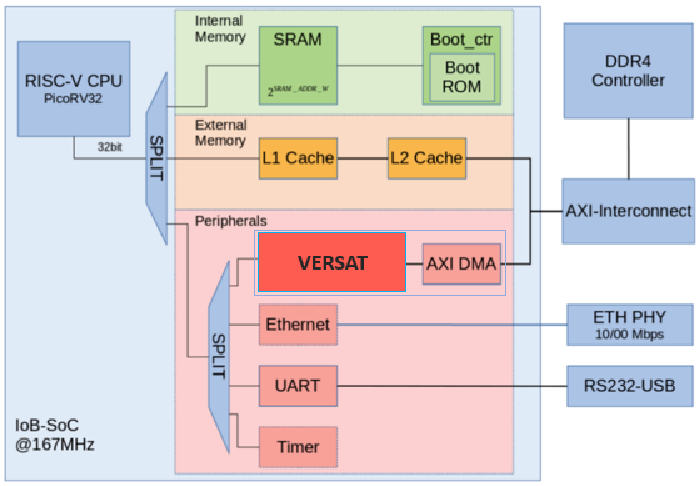
\includegraphics[width=0.85\linewidth]{iob-soc-versat.pdf}}
\caption{\textit{Versat} integrated in IOb-SoC high-level block diagram.}
\label{fig:iobversat}
\end{figure}
\end{comment}

\subsubsection{Functional units}
In practical terms, \textit{Versat} contains several functional units (FUs) in its source, all written in Verilog. Nonetheless, the user has the possibility of creating and adding new ones to the source. 
A brief description of each functional unit is provided in the table below.

\begin{table}[H]
    \centering
    \begin{tabular}{|c|p{0.7\linewidth}|}
        \hline
        \multicolumn{1}{|c|}{\textbf{FU}} & \multicolumn{1}{c|}{\textbf{Description}} \\
        \hline
        \multirow{1}{*}{\textit{Const}} & This module outputs a 32-bit value configurable by the CPU.  \\
        \hline
        \multirow{2}{*}{\textit{FloatAdd}} & This module receives two 32-bit floating-point inputs, adds them together, and outputs a 32-bit floating-point value. \\
        \hline
        \multirow{2}{*}{\textit{FloatSub}} & This module receives two 32-bit floating-point inputs, subtracts one from the other, and outputs a 32-bit floating-point value. \\
        \hline
        \multirow{2}{*}{\textit{FloatMul}} & This module receives two 32-bit floating-point inputs, multiplies them together, and outputs a 32-bit floating-point value. \\
        \hline
        \multirow{2}{*}{\textit{FloatNot}} & This module receives a 32-bit floating-point input, negates the most significant bit (MSB), and outputs a 32-bit floating-point value. \\
        \hline
        \multirow{6}{*}{\textit{Float2Int}} &  
        This module receives a 32-bit floating-point input and converts it to a 32-bit integer output. 
        It performs a conversion operation that truncates the fractional part of the floating-point input, effectively extracting the integer component. 
        The resulting 32-bit integer output represents the integer part of the input floating-point number. 
        In cases where the input is negative, the output will represent the floor of the absolute value of the input. \\
        \hline
        \multirow{4}{*}{\textit{Mux2}} & This module receives two 32-bit inputs and one 1-bit control input. 
        It operates as a 2-to-1 multiplexer, selecting one of the 32-bit inputs based on the 1-bit control input. 
        If the control input is zero, the output will be the first 32-bit input; otherwise, the output will be the second 32-bit input. \\
        \hline
        \multirow{7}{*}{\textit{Mem}} & This module contains an internal memory with two input and two output ports (True dual-port synchronous RAM). 
        It offers a memory-mapped interface that allows the CPU to store and read data from the memory while the \textit{Versat} accelerator is not running. 
        Internally, this module contains two Address Generator Units (AGU) that generate the addresses used to access the memory, one for each port. 
        The AGUs can be configured to output or store data (only one type per port, the same port cannot be configured to output and store data at the same time in one run). \\
        \hline
        \multirow{5}{*}{\textit{LookupTable}} & This module contains an internal memory with two input and two output ports (Dual port synchronous RAM). 
        It offers a memory-mapped interface that allows the CPU to store and read data from the memory while the \textit{Versat} accelerator is not running. 
        Internally, this module acts like a lookup table since the output is the value stored in the address given by the input. \\
        \hline
    \end{tabular}
    \caption{\textit{Versat} functional units.}
    \label{tab:fu}
    \end{table}
    
\vspace{0.5cm}

\subsubsection{Operators}

\textit{Versat} also contains a set of operators defined in its specification source. The operators execute either over the right operand or between the left and right operands.
In practice, this terminology just abstracts the implementation of the operators in \textit{Versat}, through functional units. 

A brief description of some operators is provided in the table below.

\begin{table}[H]
    \centering
    \begin{tabular}{|c|p{0.7\linewidth}|}
        \hline
        \multicolumn{1}{|c|}{\textbf{Operator}} & \multicolumn{1}{c|}{\textbf{Description}} \\
        \hline
        \multirow{1}{*}{\textbf{$-$}} & This operator negates the right operand.  \\
        \hline
        \multirow{1}{*}{\textbf{$\sim$}} & This operator performns binary one's complement of the right operand. \\
        \hline
        \multirow{1}{*}{\textbf{$\And$}} & This operator performs a logical AND between the left and right operands. \\
        \hline
        \multirow{2}{*}{\textbf{$\ll$}} & This operator shifts the bits of the left operand to the left by the number of positions defined by the right operand. \\
        \hline
        \multirow{1}{*}{\textbf{$\vert$}} & This operator performs a logical OR between the left and right operands. \\
        \hline
        \multirow{1}{*}{\textbf{$\wedge$}} & This operator performs a logical XOR between the left and right operands. \\
        \hline
    \end{tabular}
    \caption{\textit{Versat} operators.}
    \label{tab:op}
\end{table}

\vspace{0.5cm}

\subsubsection{Syntax}

Knowing the FUs and operators \textit{Versat} provides, it is convenient to understand how the hardware design can be developed using such resources.
Figure \ref{versatspec} shows a coding example of \textit{versatSpec.txt}, the file where the \textit{Versat} accelerator should be described.

\vspace{1cm}

\begin{figure}[H]
\centerline{\fbox{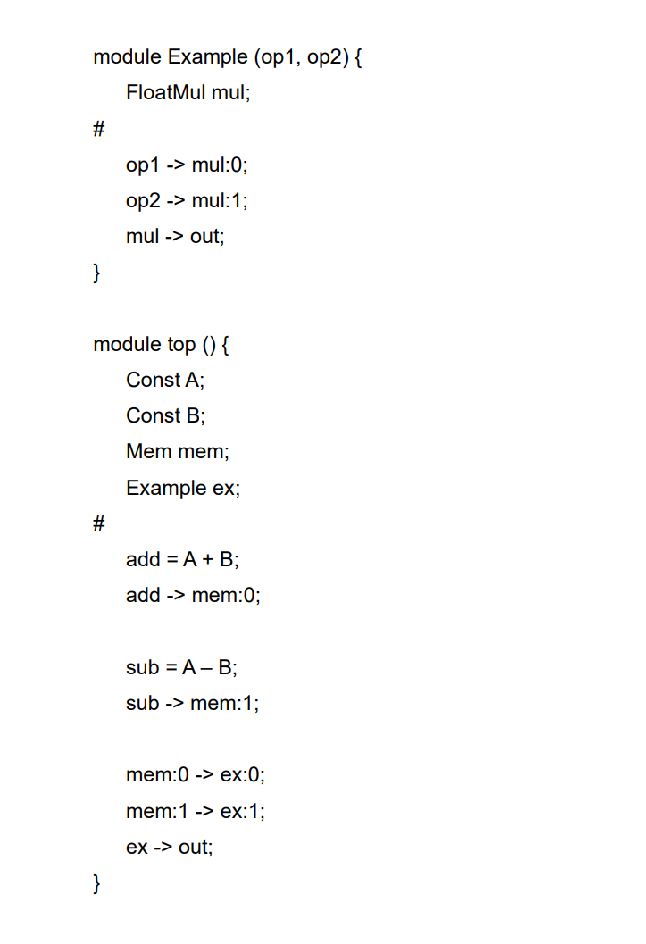
\includegraphics[width=0.60\linewidth]{versatspec.pdf}}}
\caption{\textit{versatspec.txt} example.}
\label{versatspec}
\end{figure}

Focusing on the syntax, the code is divided into two modules, \textit{Example} and \textit{top}, each representing a part of the hardware design.

The \textit{Example} module is defined with two input ports, \textit{op1} and \textit{op2}, and a \textit{FloatMul} FU, \textit{mul}. 
The code after the \# symbol specifies how data flows through the module. In this case, \textit{op1} and \textit{op2} are connected to input ports 0 and 1 of the \textit{mul} FU, respectively.  
Then, the output of the \textit{mul} FU is connected to the output port of the \textit{Example} module.

The \textit{top} module is the starting module, i.e. it represents the overall design.
This module is defined with two \textit{Const} FUs, \textit{A} and \textit{B}, and a \textit{Mem} FU, \textit{mem}. In addition, it also contains an instance of the \textit{Example} module called \textit{ex}. 
Once again, the code specifies how data flows through the modules. In this case, \textit{A} and \textit{B} are added together, and the result is stored in the \textit{add} signal. Then, \textit{add} is connected to input port 0 of the \textit{mem} FU. 
\textit{A} and \textit{B} are also subtracted, and the result is stored in the \textit{sub} signal. Then, \textit{sub} is connected to input port 1 of the \textit{mem} FU.
Afterward, the output ports 0 and 1 of \textit{mem} are connected to the input ports 0 and 1 of \textit{ex} instance, respectively. 
The \textit{ex} instance performs what was described previously for the \textit{Example} module, and its output is connected to the output port of the top module.

In terms of functionality, this example starts by performing arithmetic operations on constants \textit{A} and \textit{B}. Then, it sends the result of those operations to a memory unit, which works as an index for each input port (of the data array). Based on these indices, the memory unit outputs one value in each output port, which is then used in the following module to perform a floating-point multiplication operation. The final result is accessible through the output port of the top module.


\cleardoublepage
\section{Hardware architecture}
\label{sec:hw}
\documentclass{article}
\usepackage{diagbox}
\usepackage[utf8]{inputenc}
\usepackage{graphicx}
\usepackage[english]{babel}
\graphicspath{ {./images/} }
\usepackage{textgreek}
\usepackage{hyperref}
\usepackage{geometry}
\usepackage{caption}
\usepackage{subcaption}
\usepackage{float}
\usepackage{amsmath}
\usepackage{lmodern}
\usepackage{textcomp}
\usepackage{gensymb}
\usepackage{indentfirst}
\usepackage{array}
\usepackage{mathtools}
\usepackage{comment}
\usepackage{tabularx}
\usepackage{multirow}
\usepackage{lineno}
%\linenumbers
\DeclarePairedDelimiter{\ceil}{\lceil}{\rceil}

\makeatletter
\newcommand{\thickhline}{%
    \noalign {\ifnum 0=`}\fi \hrule height 1pt
    \futurelet \reserved@a \@xhline
}
\newcolumntype{"}{@{\vrule width 1pt}}
\makeatother

\geometry{
 a4paper,
 total={170mm,257mm},
 left=20mm,
 top=20mm}

\begin{document}

This chapter addresses the hardware architecture. It starts by setting up \textit{Versat} in the IOb-SoC. Then, it checks the \textit{Versat} Functional Units that are available in order to accelerate the \textit{psycho\_3\_threshold} function. At the end, two hardware accelerators are developed, with each one executing part of the mentioned \textit{TwoLAME} function.

\subsection{Versat}

After measuring the execution times of \textit{TwoLAME} in IOb-SoC, through profiling, it was well-marked that \textit{psycho\_3\_threshold} function needed hardware acceleration, i.e., it should be executed by custom-made hardware. This would bring the possibility to reduce between 37\% to 64\% total execution time, depending on the audio input.
At this stage, the IOb-SoC was comprising eight main components: \textbf{AXI}, \textbf{CACHE}, \textbf{LIB}, \textbf{MEM}, \textbf{VEXRISCV}, \textbf{TWOLAME}, \textbf{UART} and \textbf{TIMER}. Given \textit{Versat} being the optimal choice for accelerating the \textit{psycho\_3\_threshold} function, integration into IOb-SoC becomes imperative.
Therefore, the first step in this process was adding \textbf{VERSAT} to the IOb-SoC. This was simple as \textit{VERSAT} was previously implemented and tested by \textit{IObundle, Lda}. Apart from adding it as submodule to IOb-SoC's repository, some paths were changed to allow correct compilation.
The second step was more complex, consisting in adding an interconnection between \textit{Versat} and RAM. Iob-SoC usually contains a single AXI interface, used by both cache memory and CPU. Considering this, the solution was to double the size of the wires from the already existing AXI interface, providing an additional interface to \textit{Versat} while avoiding a new separate interface.
%explain better

\subsubsection{Functional units}
In practical terms, \textit{Versat} is a reconfigurable hardware accelerator that contains several functional units in its source, all written in Verilog. Nonetheless, the user has the possibility of creating and adding new ones to the source.
In this work, the hardware accelerators use a set of 14 functional units, of which 5 were specifically created to allow accelerating \textit{psycho\_3\_threshold} function (\textit{FloatLess}, \textit{FloatGreater}, \textit{FloatGreaterEqual}, \textit{Mux4} and \textit{Conditional1}). The remaining 9 units were already included in the units source.

A brief description of each functional unit is provided in the list below.

\vspace{0.5cm}

\textbf{\textit{Const}}
\begin{itemize}
\item This module receives a 32-bit input and outputs the same 32-bit value.
\end{itemize}

\vspace{0.5cm}

\textbf{\textit{FloatAdd}}
\begin{itemize}
\item This module receives two 32-bit floating-point inputs, adds them together, and outputs a 32-bit floating-point value.
\end{itemize}

\vspace{0.5cm}

\textbf{\textit{FloatSub}}
\begin{itemize}
\item This module receives two 32-bit floating-point inputs, subtracts one from the other, and outputs a 32-bit floating-point value.
\end{itemize}

\vspace{0.5cm}

\textbf{\textit{FloatMul}}
\begin{itemize}
\item  This module receives two 32-bit floating-point inputs, multiplies them together, and outputs a 32-bit floating-point value.
\end{itemize}

\vspace{0.5cm}

\textbf{\textit{FloatNot}}
\begin{itemize}
\item  This module receives a 32-bit floating-point input, negates the most significant bit (MSB), and outputs a 32-bit floating-point value.
\end{itemize}

\vspace{0.5cm}

\textbf{\textit{FloatLess}}
\begin{itemize}
\item  This module receives two 32-bit floating-point inputs and outputs a 32-bit value (repeated 1-bit result result 32 times) indicating whether the first input is less than the second. It performs a comparison operation to determine if the first input is less than the second.
If the first input is less than the second, the output will be a 32-bit value with all bits set to 1; otherwise, the output will be a 32-bit value with all bits set to 0.
\end{itemize}

\vspace{0.5cm}

\textbf{\textit{FloatGreater}}
\begin{itemize}
\item  This module receives two 32-bit floating-point inputs and outputs a 32-bit value (repeated 1-bit result 32 times) indicating whether the first input is greater than the second. It performs a comparison operation to determine if the first input is greater than the second.
If the first input is greater than the second, the output will be a 32-bit value with all bits set to 1; otherwise, the output will be a 32-bit value with all bits set to 0.
\end{itemize}

\vspace{0.5cm}

\textbf{\textit{FloatGreaterEqual}}
\begin{itemize}
\item  This module receives two 32-bit floating-point inputs and outputs a 32-bit value (repeated 1-bit result 32 times) indicating whether the first input is greater than or equal to the second. It performs a comparison operation to determine if the first input is greater than or equal to the second.
If the first input is greater than or equal to the second, the output will be a 32-bit value with all bits set to 1; otherwise, the output will be a 32-bit value with all bits set to 0.
\end{itemize}

\vspace{0.5cm}

\textbf{\textit{Float2Int}}
\begin{itemize}
\item  This module receives a 32-bit floating-point input and converts it to a 32-bit integer output. It performs a conversion operation that truncates the fractional part of the floating-point input, effectively extracting the integer component. The resulting 32-bit integer output represents the integer part of the input floating-point number. In cases where the input is negative, the output will represent the floor of the absolute value of the input.
\end{itemize}

\vspace{0.5cm}

\textbf{\textit{Mux2}}
\begin{itemize}
\item  This module receives two 32-bit inputs and one 1-bit control input. It operates as a 2-to-1 multiplexer, selecting one of the 32-bit inputs based on the 1-bit control input. 
If the control input is zero, the output will be the first 32-bit input; otherwise, the output will be the second 32-bit input.
\end{itemize}

\vspace{0.5cm}

\textbf{\textit{Mux4}}
\begin{itemize}
\item  This module receives four 32-bit inputs and one 32-bit control input. It operates as a 4-to-1 multiplexer, selecting one of the 32-bit inputs based on the two least significant bits (LSB) of the control input. 
The two LSB of the control input can be '00', '01', '10' or '11', selecting the first, the second, the third or the fourth input, respectively. The output will be the 32-bit input that was selected.
\end{itemize}

\vspace{0.5cm}

\textbf{\textit{Conditional1}}
\begin{itemize}
\item  This module receives two 32-bit inputs and one 32-bit control input. It operates as a 2-to-1 multiplexer, selecting one of the 32-bit inputs based on the 32-bit control input. 
If the LSB of the control input is zero, the output will be the second 32-bit input; otherwise, the output will be the first 32-bit input.
\end{itemize}

\vspace{0.5cm}

\textbf{\textit{Mem}}
\begin{itemize}
\item  This module contains an internal memory with two input and two output ports (True dual-port synchronous RAM). It offers a memory mapped interface that allows the CPU to store and read data from the memory while the \textit{Versat} accelerator is not running. 
Internally, this module contains two Address Generator Units (AGU) that generate the addresses used to access the memory, one for each port. The AGUs can be configured to output or to store data (only one type per port, the same port cannot be configured to output and store data at the same time in one run).
\end{itemize}

\vspace{0.5cm}

\textbf{\textit{LookupTable}}
\begin{itemize}
\item This module contains an internal memory with two input and two output ports (Dual port synchronous RAM). It offers a memory mapped interface that allows the CPU to store and read data from the memory while the \textit{Versat} accelerator is not running. 
Internally, this module acts like a lookup table since the output is the value stored in the address given by the input.
\end{itemize}

\vspace{0.5cm}

\subsubsection{Operators}
\textit{Versat} also contains several operators defined in its specification source. The operators execute either over the right operand or between the left and right operands.
In this work, the hardware accelerators use a set of 6 operators that were already included in the source.
A brief description of each operator is provided in the list below.

\vspace{0.5cm}

\textbf{[$-$]}
\begin{itemize}
\item  This operator negates the right operand.
\end{itemize}

\vspace{0.5cm}

\textbf{[$\sim$]}
\begin{itemize}
\item  This operator negates the MSB of the right operand.
\end{itemize}

\vspace{0.5cm}

\textbf{[$\And$]}
\begin{itemize}
\item  This operator performs a logical AND between the left and right operands.
\end{itemize}

\vspace{0.5cm}

\textbf{[$\ll$]}
\begin{itemize}
\item  This operator shifts the bits of the left operand to the left by the number of positions defined by the right operand.
\end{itemize}

\vspace{0.5cm}

\textbf{[$\vert$]}
\begin{itemize}
\item This operator performs a logical OR between the left and right operands.
\end{itemize}

\vspace{0.5cm}

\textbf{[$\wedge$]}
\begin{itemize}
\item This operator performs a logical XOR between the left and right operands.
\end{itemize}

\vspace{0.5cm}

Understanding the resources that \textit{Versat} offers, the subsequent step involves examining the \textit{psycho\_3\_threshold} function.
This function contains three for loops, with the first one being a simple initialization process, setting each element of arrays \textit{LTtm} and \textit{LTnm} to a constant value (\textit{DBMIN}) within the range of 0 to 135 ($SUBSIZE-1$). Performing this initialization in hardware incurs unnecessary overhead, as the result remains constant for all iterations. Instead, in a hardware implementation, we can directly use the constant value DBMIN as an input for the subsequent hardware operations (the next for loops, in this case), optimizing efficiency and reducing the need for a dedicated initialization loop.
Therefore, only two accelerators should be developed in order to execute the second and third for loops of \textit{psycho\_3\_threshold}.

The third for loop is simple as it just includes the \textit{psycho\_3\_add\_db} function. 
On the opposite, the second for loop is not only complex but it is also more interesting. The main for loop (outer loop) contains two \textit{if} conditions and, inside each condition, there is another for loop (inner loop). Moreover, the inner loop is the same in both conditions, differing only on part of the input data. This means that it is only necessary to develop hardware that executes both inner loops, with the if conditions and the outer loop being handled by the CPU.

\subsection{First accelerator}
Concerning hardware acceleration, a crucial step is to determine the control and data paths of the software that is intended to be accelerated. In other words, the paths refers to the fundamental components that dictate how the software interacts with the hardware to achieve acceleration.

The control path defines the flow and sequencing of operations within the software that needs to be accelerated. It includes decisions, branching, loops, and other control structures that determine the program's behavior. Determining the control path is vital for optimizing the hardware design to efficiently execute these operations.
The data path refers to the route through which data flows within the software during its execution. It involves operations and transformations applied to the input data to produce the desired output. Understanding the data path is crucial for designing hardware components that can process and manipulate the data effectively to accelerate the software's performance.

Considering this, optimizing both the control and data paths is essential to develop an efficient hardware design that aligns with the software's requirements.

\subsubsection{Control and Data paths}
This section shows both control and data paths of the first accelerator, corresponding to the second for loop in \textit{psycho\_3\_threshold} function.

\begin{figure}[H]
\centerline{\fbox{\includegraphics[width=0.90\linewidth]{first.pdf}}}
\caption{Control and data paths of the first hardware accelerator.}
\label{data1}
\end{figure}

\subsubsection{Modules}
After analysing the control and data paths, the hardware accelerator is developed in \textit{versatSpec.txt}. This file specifies the whole data process, which can be divided in several modules each representing a certain functionality or output. The starting module is called \textit{start} and invokes all the other modules.

A brief description of each module is provided in the list below.

\vspace{0.5cm}

\textit{\textbf{av}}

\begin{enumerate}

\item Float multiplication (\textit{mul1}):
\begin{itemize}
\item Takes \textit{const2} and \textit{bark} as inputs.
\item Multiplies \textit{const2} and \textit{bark}.
\end{itemize}

\item Float addition (\textit{add1}):
\begin{itemize}
\item Takes the output of \textit{mul1} and \textit{const1} as inputs.
\item Adds \textit{mul1} and \textit{const1}.
\end{itemize}

\item Float addition (\textit{add2}):
\begin{itemize}
\item Takes the output of \textit{add1} and \textit{Xtm} as inputs.
\item Adds \textit{add1} and \textit{Xtm}.
\end{itemize}

\item Float addition (\textit{add3}):
\begin{itemize}
\item Takes the output of \textit{add2} and \textit{const3} as inputs.
\item Adds \textit{add2} and \textit{const3}.
\end{itemize}

\item Output (\textit{out}):
\begin{itemize}
\item Takes the output of \textit{add3} as the final output of this module.
\end{itemize}

\end{enumerate}

\vspace{0.5cm}

\textit{\textbf{dzRange}}

\begin{enumerate}

\item Greater or equal comparison (\textit{ge1\_dzRange}):
\begin{itemize}
\item Compares the input \textit{dz} with \textit{const1\_dzRange} for greater than or equal condition.
\end{itemize}

\item Less than comparison (\textit{lt1\_dzRange}):
\begin{itemize}
\item Compares the input \textit{dz} with \textit{const2\_dzRange} for less than condition.
\end{itemize}

\item Logical AND operation (\textit{and}):
\begin{itemize}
\item Performs a logical AND operation on the outputs of \textit{ge1\_dzRange} and \textit{lt1\_dzRange}.
\end{itemize}

\item Output (\textit{out}):
\begin{itemize}
\item Takes the output of \textit{and} as the final output of this module.
\end{itemize}

\end{enumerate}

\vspace{0.5cm}

\textbf{\textit{Logic}}

\begin{enumerate}

\item Less than comparison (\textit{lt1\_Logic}, \textit{lt2\_Logic}, \textit{lt3\_Logic}):
\begin{itemize}
\item Compares the input \textit{dz} with \textit{const1\_Logic}, \textit{const2\_Logic} and \textit{const3\_Logic} for less than conditions.
\end{itemize}

\item Bitwise NOT, AND and Shift Left operations:
\begin{itemize}
\item Performs bitwise NOT, AND and Shift Left operations with the previous outputs to calculate \textit{one}.
\end{itemize}

\item Bitwise AND, OR, and Shift Left operations:
\begin{itemize}
\item Performs bitwise AND, OR, and Shift Left operations with the previous outputs to calculate \textit{zero}.
\end{itemize}

\item Bitwise XOR operation (\textit{sel}):
\begin{itemize}
\item Combines the previous outputs using bitwise XOR to obtain the final selection.
\end{itemize}

\item Output (\textit{out}):
\begin{itemize}
\item Takes the output of \textit{sel} as the final output of this module.
\end{itemize}

\end{enumerate}

\vspace{0.5cm}

\textbf{\textit{vf4}}

\begin{enumerate}

\item Calculation of $0.4 * Xtm + 6$:
\begin{itemize}
\item Multiplies \textit{Xtm} by \textit{const3\_vf4}.
\item Adds \textit{const4\_vf4} to the result.
\end{itemize}

\item Calculation of  $17 * (dz + 1) - (0.4 * Xtm + 6)$:
\begin{itemize}
\item Adds 1 to the input \textit{dz}.
\item Multiplies the result by \textit{const1\_vf4}.
\item Subtracts the output of step 1 from the previous result.
\end{itemize}

\item Calculation of  $(0.4 * Xtm + 6) * dz$:
\begin{itemize}
\item Multiplies the output of step 1 by the input \textit{dz}.
\end{itemize}

\item Calculation of  $-17 * dz$:
\begin{itemize}
\item Multiplies the input \textit{dz} by \textit{const5\_vf4}.
\end{itemize}

\item Calculation of  $-(dz - 1) * (17 - 0.15 * Xtm) - 17$:
\begin{itemize}
\item Subtracts 1 from the input \textit{dz}.
\item Multiplies the previous result by \textit{const6\_vf4}.
\item Multiplies \textit{Xtm} by \textit{const1\_vf4}.
\item Subtracts the output of step 5 from the previous result.
\end{itemize}

\item Conditional selection based on \textit{logic1}:
\begin{itemize}
\item Uses a multiplexer \textit{mux4\_vf4} to select one of the previous outputs based on the input \textit{logic1}.
\end{itemize}

\item Output (\textit{out}):
\begin{itemize}
\item Takes the output of \textit{mux4\_vf4} as the final output of this module.
\end{itemize}

\end{enumerate}

\vspace{0.5cm}

\textbf{\textit{psycho\_3\_add\_db}}

\begin{enumerate}

\item Input multiplexing (\textit{mux4\_psycho\_3}):
\begin{itemize}
\item Uses a multiplexer to select one of the inputs (\textit{a}, \textit{b}, \textit{add1}, \textit{add2}) based on the selection signal \textit{sel}.
\end{itemize}

\item Conditional selection using if condition (\textit{conditional\_psycho\_3}):
\begin{itemize}
\item Uses a conditional block to select \textit{a} or the output of \textit{mux4\_psycho\_3} based on the input \textit{if}.
\end{itemize}

\item Output (\textit{out}):
\begin{itemize}
\item Takes the output of \textit{conditional\_psycho\_3} as the final output of this module.
\end{itemize}

\end{enumerate}

\vspace{0.5cm}

\textbf{\textit{start}}

This is the main module, which is responsible for invoking all the other modules. It interconnects all modules by defining the correct inputs and outputs, apart from executing operations that are not included in any module but are required, like simple logical operations.


\subsubsection{Firmware}
Apart from specifying the data process, configuring all the input data for the hardware accelerator is also required. The inputs can either be simple constants or data arrays that are streamed by a memory unit, sequentially. The inputs can also be stored in a memory unit and accessed randomly.

As mentioned in the \textit{psycho\_3\_threshold} function section, the first accelerator executes both inner loops in the second for loop of \textit{psycho\_3\_threshold}.
Therefore, this accelerator executes several runs, i.e. there is the need to configure the accelerator with at least two sets of input data.
This is done in two separate functions because part of the data configuration is valid for all the runs. Part of the configuration that doesn't change (between runs) belongs to the \textit{initVersat} function, while the remaining part belongs to \textit{configureVersat} function.

In \textit{initVersat} the constants (that don't change between runs) are configured by assigning the intended value to the constant name (from the hardware accelerator). For floating-point data the \textit{PackInt} function is required, which receives the intended value as argument.
There is also a memory unit configuration for \textit{freq\_subset} array. This sets an internal memory with each position of the array, from 0 to SUBSIZE, read by the CPU through \textit{VersatUnitWrite} function, sequentially.
There are also two memory unit configurations for \textit{bark} and \textit{mem}$\rightarrow$\textit{dbtable} arrays. These set two lookup tables, with SUBSIZE and HBLKSIZE, respectively.

In \textit{configureVersat} four constants are configured as they differ between runs. An input of \textit{mux2} multiplexer is also configured based on a flag that is handled by the CPU.
At this point, all the input data is set for the hardware accelerator, and so it starts the execution through \textit{RunAccelerator} functions. This function receives as argument the number of times that the accelerator should run with the exact same configuration, which is 1.


\subsection{Second accelerator}

\subsubsection{Control and Data paths}
This section shows both control and data paths of the second accelerator, corresponding to the third for loop in \textit{psycho\_3\_threshold} function.

\begin{figure}[H]
\centerline{\fbox{\includegraphics[width=0.90\linewidth]{second.pdf}}}
\caption{Control and data paths of the second hardware accelerator.}
\label{data2}
\end{figure}

\subsubsection{Modules}

\vspace{0.5cm}

\textbf{\textit{psycho\_3\_add\_db\_V1}}

\begin{enumerate}

\item Input Multiplexing (\textit{mux4\_psycho\_3}):
\begin{itemize}
\item Uses a multiplexer \textit{mux4\_psycho\_3} to select one of the inputs (\textit{a}, \textit{b}, \textit{add1}, \textit{add2}) based on the selection signal \textit{sel}.
\end{itemize}

\item Output Selection (out):
\begin{itemize}
\item Takes the output of \textit{mux4\_psycho\_3} as the final output of this module. The selected input is determined by the value of \textit{sel}.
\end{itemize}

\end{enumerate}

\vspace{0.5cm}

\textbf{\textit{start1}}

This module has some similarity with the \textit{start} module of the first accelerator, since it contains most of the \textit{start} module description but duplicated.
It invokes and interconnects all the other modules, apart from executing operations like conditional operation.

A brief description of the conditional operation part is provided below.

\begin{enumerate}

\item Less than comparison (\textit{lt\_psycho\_31}):
\begin{itemize}
\item Compares the input \textit{bit\_rate} with \textit{const1} for less than condition.
\end{itemize}

\item Calculation of $ath - 12.0$ (\textit{sub1\_psycho\_31}):
\begin{itemize}
\item Subtracts the input \textit{const2} from \textit{ath}.
\end{itemize}

\item Conditional operation (\textit{conditional\_psycho\_3}):
\begin{itemize}
\item Takes the output of \textit{lt\_psycho\_31} and \textit{ath} as inputs.
\item Takes the output of \textit{conditional\_psycho\_3} as output. The selected input is determined by the value of \textit{sub1\_psycho\_31}.

\end{itemize}

\end{enumerate}

\subsubsection{Firmware}

As mentioned in the \textit{psycho\_3\_threshold} function section, the second accelerator executes the third for loop of \textit{psycho\_3\_threshold}.
The configuration of this accelerator is done inside a single function, since it performs only one run. Therefore, all the configuration belongs to \textit{configureVersat1} function.

In this function, the process is similar to the previous configuration function, since the second accelerator does not contain any functional unit that is not present in the first accelerator.

\end{document}

\cleardoublepage
\section{Software architecture}
\label{sec:sw}
This chapter addresses the software architecture.
It starts by setting up the IOb-Soc and configuring the firmware to allow execution of \textit{TwoLAME} encoding algorithm. Then, software optimizations are done to run \textit{TwoLAME} in FPGA. 
At the end, a detailed profiling analysis defines which part of the \textit{TwoLAME} software requires hardware acceleration.

Knowing beforehand that \textit{TwoLAME}~\cite{audacity} uses floating-point arithmetic (FP)~\cite{floatingpoint}, porting the software to PICORV32 CPU would not be the best option, due to its fixed-point arithmetic limitation. Therefore, the ideal option is porting \textit{TwoLAME} to \textbf{VEXRISCV} CPU, since it includes a floating-point unit (FPU)~\cite{fpu}.
In this process, the first step was removing the \textit{PICORV32} from the IOb-SoC and adding the VEXRISCV as the only CPU. This was straightforward, as \textit{VEXRISCV} was previously implemented and tested by \textit{IObundle, Lda}. Apart from adding the submodule to IOb-SoC's repository, some paths were changed to allow the correct compilation of the CPU. Interrupt signals were also added to the system data bus, such as \textit{timerInterrupt}, \textit{softwareInterrupt}, and \textit{externalInterrupt}.

\subsection{Audio test files}

Before porting the software, the \textit{TwoLAME} itself had to be verified. This verification was just in a practical way since this open-source software was already tested and approved by other users in various systems, with positive feedback. Considering this, the verification consisted of listening to an original audio file and the corresponding encoded file, produced by \textit{TwoLAME}.

%For testing purposes
To do so, four audio files were initially generated with \textit{Audacity} software~\cite{audacity}. This is free open-source audio software, compatible with GNU/Linux~\cite{gnulinux} (current working environment), and capable of multi-track audio editing and recording.
There are some reasons for having more than one testing file, preferably with different characteristics. One of them is the number of frames, which varies depending on several factors, including the audio codec being used, the settings or parameters selected for encoding, and the duration of the audio being processed (the easiest to notice). Another reason is the ability to check if the encoding software behaves the same way for different specifications, which is a crucial point as the main goal of the intended IP core is to allow real-time encoding.

Thus, the first generated file was \textit{short.wav}, using the \textit{Generate Tone} option in \textit{Audacity}. This mono audio has a sine waveform, 44.1KHz sampling rate, 16 bits per sample, and a size of 27KB (the smallest audio file in the repository).

The second generated file was \textit{long.wav}, using the \textit{Generate Rhythm Track} option configured with \textit{Metronome Tick} beat sound in \textit{Audacity}. This mono audio has a 44.1KHz sampling rate, 16 bits per sample, and a size of 683KB.

The third generated file was \textit{noise.wav}, using the \textit{Generate Noise} option configured with \textit{White} noise type in \textit{Audacity}. This audio has a 44.1KHz sampling rate, 16 bits per sample, a size of 529KB and, unlike the previous ones, it is stereo. The mono default track was duplicated, with one being distributed 100\% to the Left and the other being distributed 100\% to the Right (\textit{panning effect}).

The fourth and last generated file was \textit{vivaldi.wav}. This file was not generated from scratch in \textit{Audacity}. Instead, it was simply converted to WAV format. The original file, entitled 'Vivaldi - Spring', was downloaded from the Internet (for free) and opened on \textit{Audacity}. After that, the track was reduced to the initial 4 seconds and exported as WAV, being also stereo. What motivated the use of this file was the recognized quality and complexity of \textit{Vivaldi}'s songs~\cite{vivaldi}.

With four audio files available at the repository, it was possible to verify the \textit{TwoLAME} software. Using a standard \textit{automake} process, composed of \textit{./configure}, \textit{make}, and \textit{make install} commands, \textit{TwoLAME} was successfully installed. Then, by simply typing \textit{stwolame} followed by the input file name, white space, and the output file name (the one desired), the software would run and produce an MP2-encoded version of the original file.
It is important to mention that both input and output file names should include the file extension. For this work, the relevant extensions are '.wav' as input and '.mp2' as output.
From executing \textit{stwolame short.wav short.mp2} command, it was verified that both the original and the encoded audio files sound the same (for a human listener). The same happened with the second and fourth files through a similar command. 
The third file is not audible, in the way that it was created just to verify proper correctness in terms of values produced. This is because white noise is the worst-case scenario for audio encoding, mainly due to its high requirements. \\


After testing the original \textit{TwoLAME} software, it was necessary to implement it in IOb-SoC. The porting of the software requires a front end, as the encoding process uses functions of \textit{libtwolame} (\textit{TwoLAME}'s library). 

\subsection{Firmware}

The front end should instantiate all the required functions to produce an MP2 audio. Considering this, the \textit{simplefrontend} example was taken from the \textit{TwoLAME} repository, improved, and implemented in \textit{firmware.c}.
%doesnt have a file system
To realize what modifications are necessary to run \textit{TwoLAME} in IOb-SoC, figure \ref{newpseudo} shows the pseudo code for the \textit{main()} function in \textit{firmware.c}.

\begin{figure}[H]
\centerline{\fbox{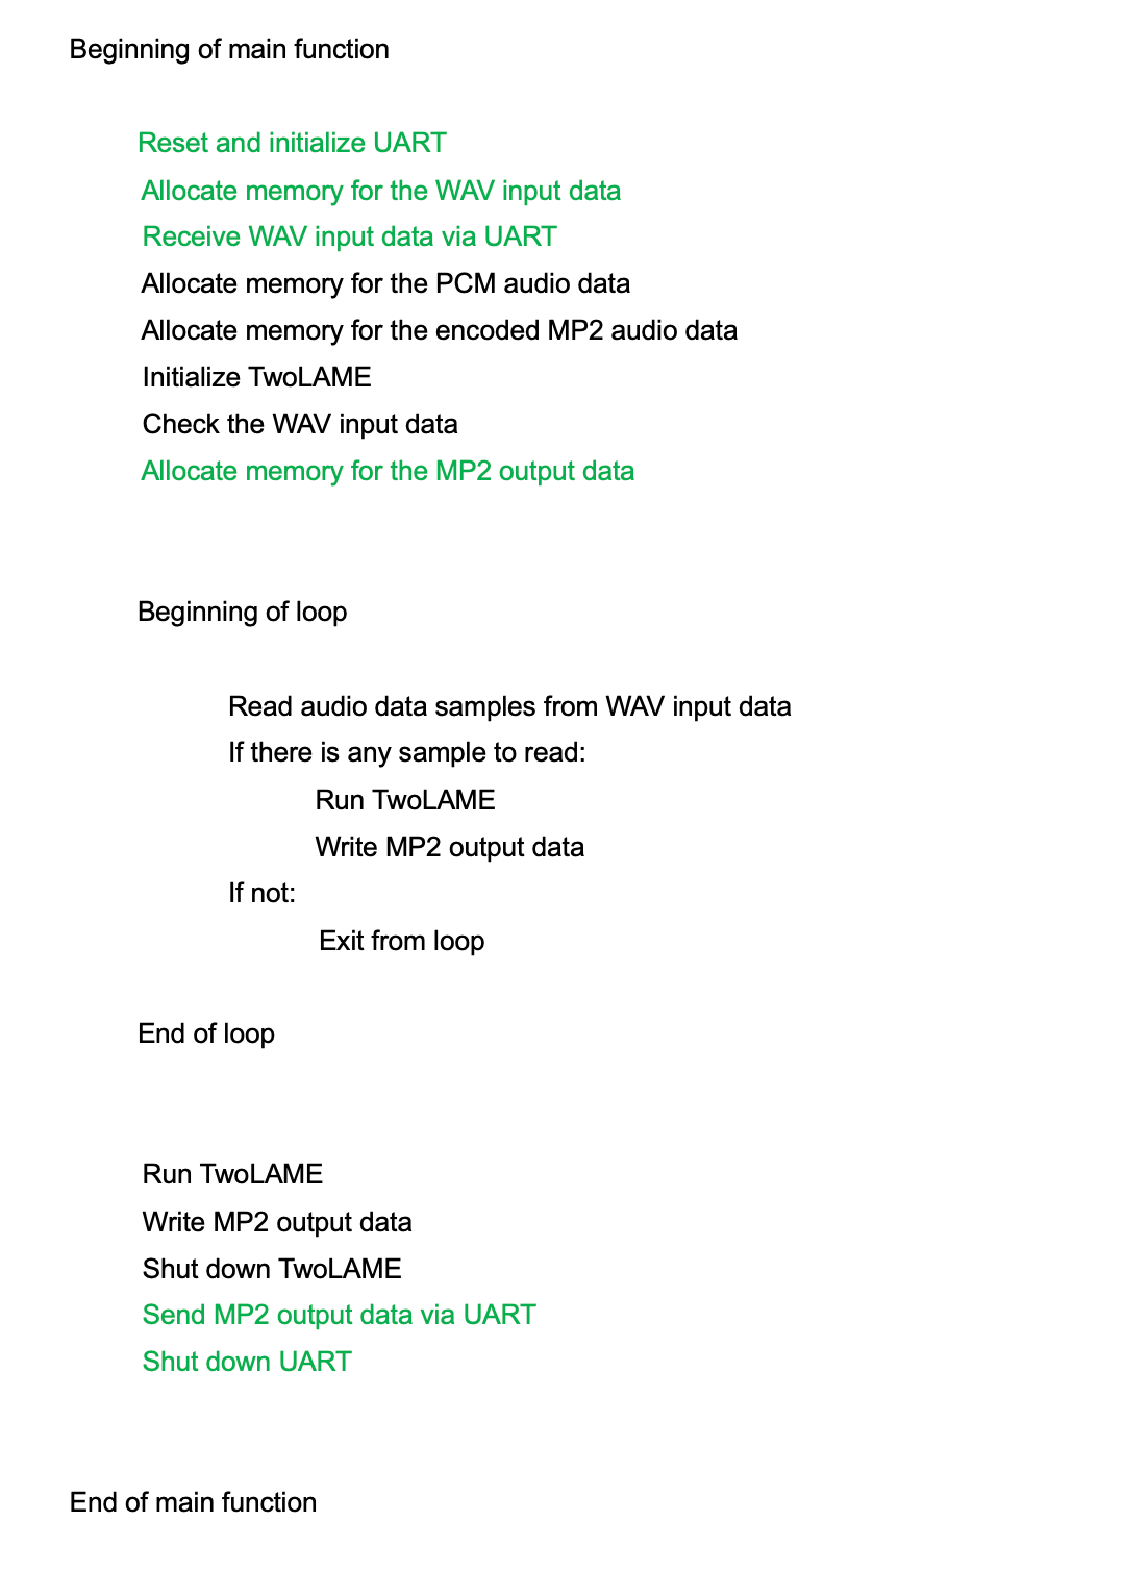
\includegraphics[width=0.80\linewidth]{newpseudo.pdf}}}
\caption{New \textit{firmware.c} pseudo code.}
\label{newpseudo}
\end{figure}

The first difference in \textit{main()} is the usage of \textit{uart\_init}, which resets \textit{IObundle, Lda}’s UART peripheral and sets its division factor. This peripheral is needed to transmit data between IOb-UART and IOb-Console. 
There are also two additional memory allocations for the input and output data. These operations are done through \textit{malloc} using unsigned char type because UART peripheral does transmit one byte at a time.
After allocating memory, the input audio data is received via UART in \textit{uart\_recvfile}. The function receives the path as an argument, which is defined as \textit{test.wav}. This is a generic name since the input audio file is copied to the compiling directory as \textit{test.wav}.
The previous modifications were done because the IOb-SoC does not have an operating system or file system. For this reason, the \textit{fopen} function inside \textit{wave\_init} was removed. Furthermore, in each iteration of the \textit{while} loop, a chunk of input data is read from the input data using \textit{fread}. Since this function, present in \textit{wave\_get\_samples}, also requires a file system, there should be some process to increment the pointer to the input data, so that \textit{fread} can be removed. This is achieved by decrementing a global variable (unread\_data) based on the number of samples read in each loop iteration. In addition, since the \textit{pcmaudio} buffer should contain short integers, there is a process inside \textit{wave\_get\_samples} that converts every two characters into a single short integer. This is done by concatenating two characters, with the first one shifted left eight positions.

Nonetheless, not only the input audio data is received via UART but also the output audio data is sent via UART. Thus, the \textit{fwrite} functions were also removed from \textit{main}.
More precisely, there was one situation inside the \textit{while} loop and another after the loop, with both \textit{memcpy} insertions being responsible for writing the MP2 output data, replacing \textit{fwrite} calls. An important detail about this modification comes with the pointer to the output data. Just like in \textit{wave\_get\_samples}, there should be a process to increment the pointer to the output data, so that the new data does not overwrite previous data. This process is based on the number of frames encoded in each loop iteration, specifically inside \textit{\textit{TwoLAME}\_encode\_buffer\_interleaved} function.
One of the last modifications in \textit{main} consists of sending the output data via UART in \textit{uart\_sendfile}. The function receives the path as an argument, which is defined as ’../../encoded.mp2’. This way, the output audio file is copied to the main repository directory as \textit{encoded.mp2}.
Afterward, the UART transmission is closed through \textit{uart\_finish}, and the program returns.

Apart from main(), some header files were included in \textit{firmware.c}, related to both the IOb-SoC system and \textit{TwoLAME} front end. Two macros were also defined, AUDIOBUFSIZE as 2304 and MP2BUFSIZE as 4096. These variables specify the size of input and output buffers, respectively, which in practice represent the chunk of data encoded each time (the number of frames encoded). Therefore, the number of frames can be altered by changing both variables on the same scale. As it stands, the \textit{TwoLAME} encodes one frame at a time.


\subsection{Optimization}

With the \textit{TwoLAME} already implemented in firmware.c, it is possible to emulate the program, by running it on a PC. It is also possible to simulate its execution on a PC. However, the major interest is in running \textit{TwoLAME} in FPGA, as the goal is to encode MP2 audio in real time. Considering this, some basic software improvements were done before evaluating the performance in FPGA.

The first change in \textit{libtwolame} was the software precision. In \textit{comon.h}, there is a macro for FLOAT that was initially defined as \textit{double}, but it was changed to \textit{float}. One reason for this is the fact that \textit{TwoLAME} should be faster rather than more accurate, without compromising the encoded audio quality. The other reason was IOb-SoC does not support double precision~\cite{doubleprecision}, since it contains floating-point units with single precision, exclusively. Apart from altering the macro, one function in \textit{subband.c} was also changed. The original code contained \textit{modf}~\cite{modf}, a function that belongs to \textit{math.h}~\cite{mathh} and requires double precision. Therefore, it was substituted by \textit{modff}~\cite{modf}, which has the same functionality (returns the fractional part) but uses single precision.

The second change was more strategic, as it involved a more careful analysis of the encoding software. It is known that trigonometric functions~\cite{trigonometric} are computationally complex, and \textit{TwoLAME}, as an audio-processing software, requires different mathematical functions. For this reason, some math functions were removed and substituted by tables, wherever it was possible. To evaluate this possibility, the \textit{TwoLAME} was emulated on a PC, and compiled with different test files.

The first case was \textit{psycho\_3\_powerdensityspectrum}, in \textit{psycho\_3.c}. In this function, there was a \textit{log10} operation inside a \textit{i} loop, with \textit{i} ranging from 1 to 512 (HBLKSIZE-1). Since the \textit{log10} operation was performed based on \textit{energy[i]}, the solution was creating a table with 512 positions, so that \textit{energy[i]} determines the index that should be accessed from the table. To be linear access, \textit{energy[i]} has to be multiplied by 1000 and converted to an integer. Since it is guaranteed that in the \textit{else} condition the array value is always positive, a condition was added to upper limit the index of the log10 table (511 is the maximum index). With this, and noticing the multiplication by 10 (of log10) in the original code, the \textit{tablog10\_psycho\_3\_powerdensityspectrum} was created by calculating $LOG10(x/10000)$ in an excel sheet, with \textit{x} ranging from 0 and 511. It was then copied and defined in \textit{psycho\_3.c}, with a change in index 0. Since \textit{log10(0)=-inf}, the first index in the table was defined as -40 (the same value as index 1).

\begin{comment}
\begin{figure}[H]
\centerline{\fbox{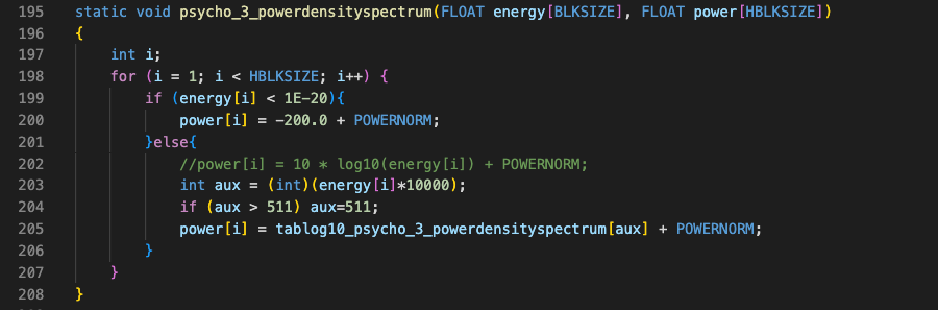
\includegraphics[width=0.80\linewidth]{powerdensityspectrum.pdf}}}
\caption{\textit{psycho\_3\_powerdensityspectrum} function.}
\label{powerdensityspectrum}
\end{figure}
\end{comment}

%\vspace{1cm}

The second case was \textit{psycho\_3\_init\_add\_db}, also in \textit{psycho\_3.c}. In this function, there were both \textit{pow} and \textit{log10} operations inside a \textit{i} loop, with \textit{i} ranging from 0 to 999 (DBTAB-1). However, this case was straightforward to solve, since the result produced in each iteration does not depend on any input data. Considering this, the \textit{tablog10\_psycho\_3\_init\_add\_db} was created by calculating the whole expression in an excel sheet, with \textit{x} ranging from 0 to 99.9 ($x=i/10.0$).

\begin{comment}
\begin{figure}[H]
\centerline{\fbox{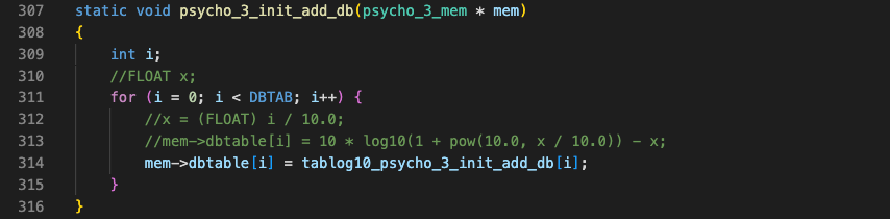
\includegraphics[width=0.80\linewidth]{init.pdf}}}
\caption{\textit{psycho\_3\_init\_add\_db} function.}
\label{init}
\end{figure}
\end{comment}

%\vspace{1cm}

The third case was \textit{psycho\_3\_spl}, in \textit{psycho\_3.c}. In this function, there was a \textit{log10} operation inside a \textit{i} loop, with \textit{i} ranging from 0 to 31 (SBLIMIT-1). Since the \textit{log10} operation was performed based on \textit{scale[i]} and its value was never higher than 20000 (after being multiplied by 32768), the solution was creating a table with 2000 positions, so that \textit{scale[i]} determines the index that should be accessed from the table. 
To be linear access, \textit{scale[i]} has to be multiplied by 3276.8 and converted to an integer. Since it is guaranteed that the array value is always positive, a condition was added to limit the index of the log10 table (1999 is the maximum index). With this, and noticing the multiplication by 20 followed by the subtraction by 10 (of log10) in the original code, the \textit{tablog10\_psycho\_3\_spl} was created by calculating $20\times log10(x\times 10)-10$ in an excel sheet, with \textit{x} ranging from 0 and 1999. It was then copied and defined in \textit{psycho\_3.c}.

\begin{comment}
\begin{figure}[H]
\centerline{\fbox{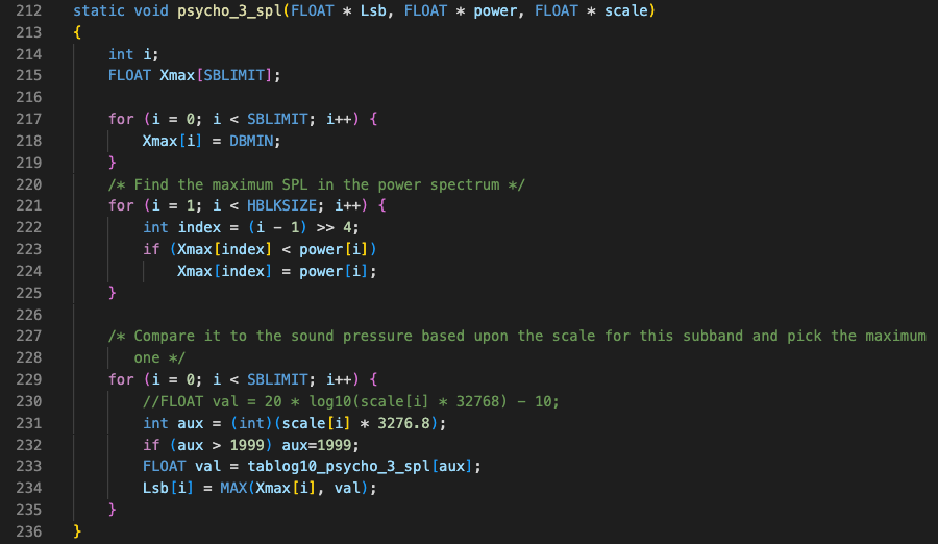
\includegraphics[width=0.80\linewidth]{spl.pdf}}}
\caption{\textit{psycho\_3\_spl} function.}
\label{spl}
\end{figure}

\vspace{1cm}
\end{comment}

The fourth case was \textit{psycho\_3\_fft}, in \textit{psycho\_3.c} too. In this function, there was a \textit{pow} operation and also a \textit{cos} operation inside a \textit{i} loop, with \textit{i} ranging from 0 to 1023 (BLKSIZE-1). This case was straightforward to solve since the result produced in each iteration does not depend on any input data. Considering this, the \textit{tabcos\_psycho\_3\_fft} was created by calculating both expressions in an Excel sheet, with \textit{x} ranging from 0 to 1023.

\begin{comment}
\begin{figure}[H]
\centerline{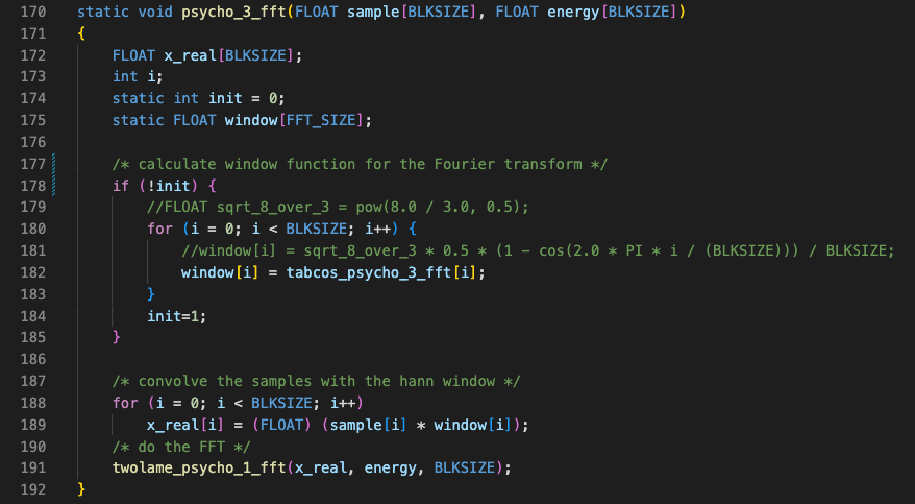
\includegraphics[width=0.80\linewidth]{fft.pdf}}
\caption{\textit{psycho\_3\_fft} function.}
\label{fft}
\end{figure}

\vspace{1cm}
\end{comment}

The fifth and last case was \textit{create\_dct\_matrix}, in \textit{subband.c}. In this function, there was a \textit{cos} operation inside a nested loop, with \textit{i} ranging from 0 to 15 and \textit{k} ranging from 0 to 31. This case was also straightforward to solve since the result produced in each iteration does not depend on any input data. Considering this, the \textit{tabcos\_create\_dct\_matrix} was created by calculating the whole expression in an Excel sheet, with \textit{aux} ranging from 0 to 511 ($16 \times 32$).

\begin{comment}
\begin{figure}[H]
\centerline{\fbox{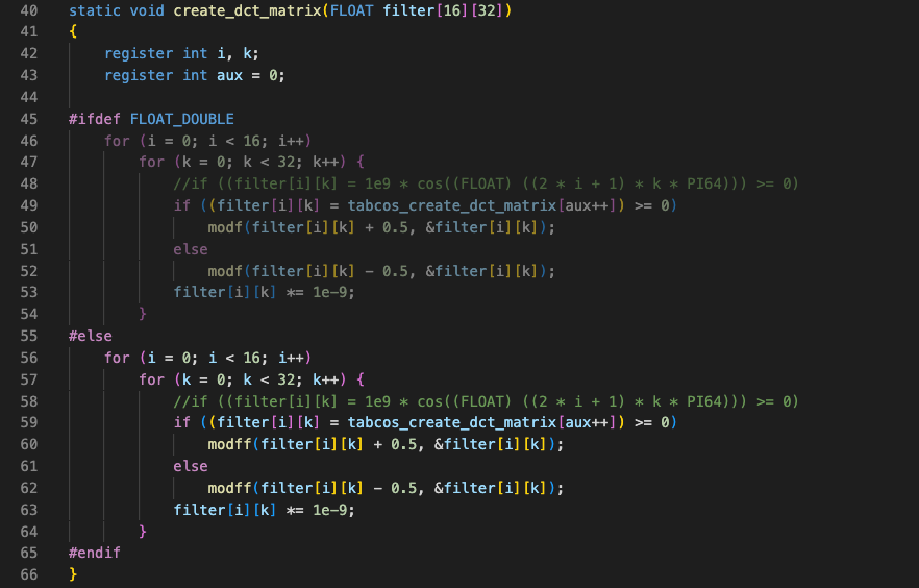
\includegraphics[width=0.80\linewidth]{dct.pdf}}}
\caption{\textit{create\_dct\_matrix} function.}
\label{dct}
\end{figure}

\vspace{1cm}
\end{comment}

The third and last change in \textit{libtwolame} was related to memory.
Initially, there was a memory allocation for \textit{bit\_stream} struct in \textit{twolame\_buffer\_init}, called from \textit{twolame\_encode\_buffer\_interleaved} function. Since this function executes in every \textit{while} loop iteration, in \textit{firmware.c}, the memory allocation was also performed many times.
Therefore, the \textit{TWOLAME\_MALLOC} of \textit{bit\_stream} struct was moved to the \textit{main} function, meaning that it executes just once before the encoding process starts.
In addition, the \textit{TWOLAME\_FREE} in \textit{twolame\_buffer\_deinit}, called from \textit{twolame\_encode\_buffer\_interleaved}, was removed and, consequently, added to \textit{main}.

%grep -r 'tab' *

%\subsection{FPGA}

With basic software optimizations already implemented, it is desired to measure the execution time of the \textit{TwoLAME} software for different input data. This requires different memory management since the FPGA has memory space available, and so allocating memory during program execution is not ideal, except in special cases. Considering this, a macro called \textit{PC\_EMUL\_RUN} is defined to control each memory allocation, through an if directive. In the first case when the program is emulated on PC, \textit{PC\_EMUL\_RUN} should be defined. In a second case when the program runs in FPGA, \textit{PC\_EMUL\_RUN} should not be defined.
Focusing on the second case, the memory space available starts at \textit{DATA\_BASE\_ADDR}. This macro defines the base address based on IOb-SoC macros from \textit{config.mk}, the IOb-SoC configuration script (explained in the next section).
In \textit{main()}, the first example is \textit{recvfile\_ch} pointer, which represents where the input data is stored in memory. As it is the first, it should be equal to \textit{DATA\_BASE\_ADDR}.
The second example is \textit{pcmaudio} pointer, which represents where the input data buffer is stored. As it is the second, it should be equal to DATA\_BASE\_ADDR + recv\_file\_size (the size of the input file).
The third example is \textit{mp2buffer} pointer, which represents where the encoded data buffer is stored. It should be equal to $pcmaudio + AUDIObUFSIZE*sizeof(short)$ (the second pointer plus the size of the input data buffer).
The fourth example is \textit{mybs} pointer, which represents where the bit\_stream struct is stored. It should be equal to $mp2buffer + MP2BUFSIZE*sizeof(unsigned char)$ (the third pointer plus the size of the encoded data buffer).
The fifth and last example is \textit{outfile} pointer, which represents where the encoded MP2 data is stored. It should be equal to $mybs + sizeof(bit\_stream)$ (the fourth pointer plus the size of the \textit{bit\_stream} struct).
In addition, the \textit{free()} functions were also inserted in a \textit{\#ifdef PC\_EMUL\_RUN} directive, since the function should only be called when the memory is dynamically allocated. \\

\subsection{Profiling}

With everything set up, the last implementation in the software architecture was \textbf{profiling}~\cite{profiling}. This process is a form of dynamic program analysis that can measure different variables, like memory space or time complexity. In this case, it was used to measure the duration of each function.
To do so, an eight component was added to IOb-SoC, the \textbf{TIMER}~\cite{bib:iobtimer}. This peripheral is a 64-bit hardware timer, equipped with reset, enable, and reading functions. It includes a software driver and an example C application, which helps understand how it works. 
Similarly to the other components, the TIMER is tracked by a \textit{GitHub} repository (forked from \textit{IObundle, Lda}), integrating the IOb-SoC as a submodule. This component was previously implemented and tested by \textit{IObundle, Lda} as well. In addition, some paths were added to allow correct compilation.

With this, IOb-SoC was ready for profiling. The process consisted of three phases, with the first phase being a more high-level approach. 
This phase was simple since only the function calls directly made from \textit{main()} were considered. The timer was first initialized through \textit{timer\_init(TIMER\_BASE)} function. Then, a \textit{elapsed\_time} integer array of size 50 was declared and set with zero. In the profiling itself, some basic operations were used for each function call. Immediately before a function call, \textit{timer\_time\_ms()} is invoked, returning the current time in ms which is then stored in \textit{start\_elapse\_time} variable as an unsigned integer. Immediately after a function call, \textit{timer\_time\_ms()} is invoked again, returning the current time in ms which is then stored in \textit{end\_elapse\_time} variable as an unsigned integer as well. Then, the difference between both variables is calculated and stored in a certain index of \textit{elapsed\_time} array (one index for each function call). 
By doing this, 13 functions were included in the first phase of \textit{TwoLAME} profiling. At the end of \textit{main()}, every position of the array is printed, showing how many ms each function call took. The printing does not influence the profiling, as it is done after the last function measurement. Another interesting detail is that both \textit{uart\_recvfile} and \textit{uart\_sendfile} functions are excluded from the profiling, which is correct since they perform data transfers that are not part of the \textit{TwoLAME}.
Table \ref{profiling1} shows the first phase of the profiling for all input files.

\begin{table}[H]
    \centering
    \begin{tabular}{c|c|c|c|c|}
    \cline{2-5}
    \multicolumn{1}{c|}{}  & \multicolumn{4}{c|}{\textbf{Input file}} \\
    \cline{2-5}
     & short.wav & long.wav & noise.wav & vivaldi.wav \\
    \hline
    \multicolumn{1}{|c|}{twolame\_init()}  & 3 & 2 & 3 & 0 \\ 
    \hline
    \multicolumn{1}{|c|}{wave\_init()}  & 0 & 0 & 0 & 0 \\ 
    \hline
    \multicolumn{1}{|c|}{twolame\_set\_num\_channels()}   & 0 & 0 & 0 & 0 \\ 
    \hline
    \multicolumn{1}{|c|}{twolame\_set\_in\_samplerate()}   & 0 & 0 & 0 & 0 \\ 
    \hline
    \multicolumn{1}{|c|}{twolame\_set\_bitrate()}   & 0 & 0 & 0 & 0 \\ 
    \hline
    \multicolumn{1}{|c|}{twolame\_init\_params()}   & 11 & 11 & 11 & 11 \\ 
    \hline
    \multicolumn{1}{|c|}{wave\_get\_samples()}   & 4 & 126 & 89 & 135 \\ 
    \hline
    \multicolumn{1}{|c|}{twolame\_encode\_buffer\_interleaved()}   & 1510 & 24345 & 19820 & 26010 \\ 
    \hline
    \multicolumn{1}{|c|}{memcpy()}  & 2 & 59 & 19 & 32 \\ 
    \hline
    \multicolumn{1}{|c|}{twolame\_encode\_flush()}   & 79 & 80 & 185 & 155 \\ 
    \hline
    \multicolumn{1}{|c|}{memcpy()}  & 0 & 0 & 0 & 0 \\ 
    \hline
    \multicolumn{1}{|c|}{twolame\_close()}   & 0 & 0 & 0 & 1 \\ 
    \hline
    \multicolumn{1}{|c|}{\textbf{\textit{TwoLAME} total}}  & 1614 & 24719 & 20210 & 26467 \\ 
    \hline
    \end{tabular}
    \caption{Execution time for all input files (first phase of \textit{profiling}) [ms].}
    \label{profiling1}
\end{table}

\vspace{1cm}


The previous table shows that \textit{twolame\_encode\_buffer\_interleaved} occupies most of the execution time, which is expected as it is responsible for the encoding, calling many other \textit{TwoLAME} functions. Nonetheless, this information is not enough, mainly because developing hardware to accelerate the whole function would be an extremely difficult task.
By analyzing \textit{twolame\_encode\_buffer\_interleaved}, it is noticeable that the relevant operation inside the function is \textit{encode\_frame()}, as all the other operations are basic.
Considering this, the second phase of profiling includes all function calls inside \textit{encode\_frame}. 
This phase was similar to the previous one in terms of methodology. The only differences were the usage of the \textit{elapsed\_time\_twolame} array, which was declared and set to 0 in \textit{main()} and passed as an argument to \textit{twolame\_encode\_buffer\_interleaved} and \textit{encode\_frame()}, consecutively. The variables that store the time values are also different, being \textit{start\_elapse\_time\_twolame} and \textit{end\_elapse\_time\_twolame}, declared in \textit{twolame.c} as global unsigned integers.
By doing this, 23 functions were included in the second phase of \textit{TwoLAME} profiling. It was not 23 functions but 23 blocks of code from \textit{encode\_frame()}, because apart from the \textit{libtwolame} functions, there is additional code that has to be included for correct measurements, like if conditions and \textit{for} loops.
At the end of \textit{main()}, every position of the array is printed, showing how many ms each part of \textit{encode\_frame()} took. 
Table \ref{profiling2} shows the second phase of the profiling for all input files.

\begin{table}[H]
    \centering
    \begin{tabular}{|c|c|c|c|c|c|}
    \cline{3-6}
    \multicolumn{2}{c|}{}  & \multicolumn{4}{c|}{\textbf{Input file}} \\
    \cline{3-6}
    \multicolumn{2}{c|}{} & \textit{short.wav} & \textit{long.wav} & \textit{noise.wav} & \textit{vivaldi.wav} \\
    \cline{1-6}
   \multirow{23}{*}{\parbox{2.5cm}{\centering \textbf{twolame} \\ \textbf{\_encode} \\ \textbf{\_buffer} \\ \textbf{\_interleaved()}}}  & \multicolumn{1}{c|}{\textit{scale\_and\_mix\_samples}}  & 0 & 9 & 5 & 3 \\ 
    \cline{2-6}
    & \multicolumn{1}{c|}{\textit{twolame\_buffer\_sstell}} & 3 & 139 & 52 & 78 \\ 
    \cline{2-6}
    & \multicolumn{1}{c|}{\textit{twolame\_available\_bits}} & 0 & 16 & 7 & 8  \\ 
    \cline{2-6}
    & \multicolumn{1}{c|}{\textit{twolame\_window\_filter\_subband}} & 141  & 3487 & 2590 & 3662  \\ 
    \cline{2-6}
    & \multicolumn{1}{c|}{\textit{twolame\_scalefactor\_calc}} & 7 & 172 & 142 &  201  \\ 
    \cline{2-6}
    & \multicolumn{1}{c|}{\textit{twolame\_find\_sf\_max}} & 0  & 13 & 3 & 6   \\ 
    \cline{2-6}
    & \multicolumn{1}{c|}{\textit{twolame\_scalefactor\_calc}} & 0  & 5 & 6 & 4  \\ 
    \cline{2-6}
     & \multicolumn{1}{c|}{\textit{twolame\_psycho\_3}} & 1377  & 19062 & 16222 &  20829 \\ 
    \cline{2-6}
    & \multicolumn{1}{c|}{\textit{twolame\_sf\_transmission\_pattern}} & 0 & 17 & 8 &  10 \\ 
    \cline{2-6}
    & \multicolumn{1}{c|}{\textit{twolame\_main\_bit\_allocation}} & 16  & 424 & 343 & 485  \\ 
    \cline{2-6}
    & \multicolumn{1}{c|}{\textit{twolame\_write\_header}} & 2 & 12 & 7 &  7 \\
    \cline{2-6}
    & \multicolumn{1}{c|}{\textit{buffer\_putbits}} & 0 & 4 & 1 & 4  \\
    \cline{2-6}
    & \multicolumn{1}{c|}{\textit{twolame\_write\_bit\_alloc}} & 0 & 11 & 11 &  17 \\
    \cline{2-6}
    & \multicolumn{1}{c|}{\textit{twolame\_write\_scalefactors}} & 1 & 22 & 20 & 27 \\
    \cline{2-6}
    & \multicolumn{1}{c|}{\textit{twolame\_subband\_quantization}} & 21 & 503 & 346 & 488 \\
    \cline{2-6}
    & \multicolumn{1}{c|}{\textit{twolame\_write\_samples}} & 12 & 306 & 149 & 210 \\
    \cline{2-6}
    & \multicolumn{1}{c|}{\textit{buffer\_put1bit}} & 0 & 10 & 4 & 2 \\
    \cline{2-6}
    & \multicolumn{1}{c|}{\textit{buffer\_putbits}} & 0 & 5 & 4 & 2 \\
    \cline{2-6}
    & \multicolumn{1}{c|}{\textit{twolame\_dab\_crc\_calc}} & 0 & 9 & 3 &  3 \\
    \cline{2-6}
    & \multicolumn{1}{c|}{\textit{buffer\_put1bit}} & 0 & 3 & 0 &  0 \\
    \cline{2-6}
    & \multicolumn{1}{c|}{\textit{twolame\_buffer\_sstell}} & 0 & 1 & 0 & 1  \\
    \cline{2-6}
    & \multicolumn{1}{c|}{\textit{twolame\_do\_energy\_levels}} & 0 & 7 & 1 & 3  \\
    \cline{2-6}
    & \multicolumn{1}{c|}{\textit{twolame\_crc\_writeheader}} & 0 & 3 & 1 &  2  \\ 
    \hline
    \multicolumn{2}{|c|}{\textbf{\textit{TwoLAME} total}}  & 1614 & 24719 & 20210 & 26467 \\ 
    \hline
    \end{tabular}
    \caption{Execution time for all input files (second phase of \textit{profiling}) [ms].}
    \label{profiling2}
\end{table}

\vspace{1cm}

The previous table shows that the eight block of \textit{encode\_frame()} occupies most of the execution time, which includes two nested loops (executed depending on \textit{if} conditions) and a switch case. The nested loops perform simple operations, so they are not relevant. The switch case calls a certain function depending on the switch condition. However, after inspecting \textit{glopts->psymodel} condition it is perceptible that case 3 is always selected, calling \textit{twolame\_psycho\_3}. Nevertheless, this information is still not enough. 
Looking at \textit{twolame\_psycho\_3}, there are many other \textit{libtwolame} functions inside it. Considering this, the third phase of profiling includes all function calls inside \textit{twolame\_psycho\_3}. 
This phase was also similar to the previous ones in terms of methodology. The only differences were the usage of the \textit{elapsed\_time\_psycho\_3} array, which was declared and set to 0 in \textit{main()} and passed as argument to \textit{twolame\_encode\_buffer\_interleaved}, \textit{encode\_frame()} and \textit{twolame\_psycho\_3}, consecutively. The variables that stored the time values were also different, being \textit{start\_elapse\_time\_psycho\_3} and \textit{end\_elapse\_time\_psycho\_3}, declared in \textit{twolame.c} as global unsigned integers.
By doing this, 13 blocks of code were included in the third phase of \textit{TwoLAME} profiling, with most of them being just functions.
At the end of \textit{main()}, every position of the array is printed, showing how many ms each block of \textit{twolame\_psycho\_3} took. 
Table \ref{profiling3} shows the third phase of the profiling for all input files.

\begin{table}[H]
    \centering
    \begin{tabular}{|c|c|c|c|c|c|}
    \cline{3-6}
    \multicolumn{2}{c|}{}  & \multicolumn{4}{c|}{\textbf{Input file}} \\
    \cline{3-6}
    \multicolumn{2}{c|}{} & short.wav & long.wav & noise.wav & vivaldi.wav \\
    \cline{1-6}
   \multirow{13}{*}{\parbox{2.3cm}{\centering \textbf{\textit{twolame\_} \\ \textit{psycho\_3}}}}  & \multicolumn{1}{c|}{twolame\_psycho\_3\_init}  & 635 & 642 & 635 & 635 \\ 
    \cline{2-6}
    & \multicolumn{1}{c|}{\textit{mem} $\rightarrow$ \textit{fft\_buf}} & 5 & 133 & 115 & 155 \\ 
    \cline{2-6}
    & \multicolumn{1}{c|}{\textit{mem} $\rightarrow$ \textit{fft\_buf}} &  6 &  117& 77 &  120 \\ 
    \cline{2-6}
    & \multicolumn{1}{c|}{\textit{psycho\_3\_fft}} & 47 & 1138 & 886 &  1253  \\ 
    \cline{2-6}
    & \multicolumn{1}{c|}{\textit{psycho\_3\_powerdensityspectrum}} & 40  & 1026 & 791 &  1115  \\ 
    \cline{2-6}
    & \multicolumn{1}{c|}{\textit{psycho\_3\_spl}} &  7 & 170 & 148 & 204  \\ 
    \cline{2-6}
     & \multicolumn{1}{c|}{\textit{psycho\_3\_tonal\_label}} &  7 & 153 & 258 & 173  \\ 
    \cline{2-6}
    & \multicolumn{1}{c|}{\textit{psycho\_3\_noise\_label}} & 8 & 220 & 167 & 235  \\ 
    \cline{2-6}
    & \multicolumn{1}{c|}{\textit{psycho\_3\_dump}} &  0 & 4 & 2 & 4  \\ 
    \cline{2-6}
    & \multicolumn{1}{c|}{\textit{psycho\_3\_decimation}} & 3 & 45 & 38 & 67   \\
    \cline{2-6}
    & \multicolumn{1}{c|}{\textit{psycho\_3\_threshold}} & 611 & 15168  & 12975 &  16684 \\
    \cline{2-6}
    & \multicolumn{1}{c|}{\textit{psycho\_3\_minimummasking}} & 0 & 23 & 14 & 29  \\ 
    \cline{2-6}
    & \multicolumn{1}{c|}{\textit{psycho\_3\_smr}} & 0 & 9 & 6 & 13  \\ 
    \hline
    \multicolumn{2}{|c|}{\textbf{\textit{TwoLAME} total}}  & 1614 & 24719 & 20210 & 26467 \\ 
    \hline
    \end{tabular}
    \caption{Execution time for all input files (third phase of \textit{profiling}) [ms].}
    \label{profiling3}
\end{table}

\vspace{1cm}

The previous table shows interesting information. First, it is noticeable that several functions have an insignificant execution time, compared to others. Second, it is clear that \textit{psycho\_3 function 11}, which is \textit{psycho\_3\_threshold}, occupies the biggest part of the program execution. For \textit{short.wav}, \textit{long.wav}, \textit{noise.wav} and \textit{vivaldi.wav}, this function corresponds to 37\%, 61\%, 64\% and 63\% of \textit{TwoLAME} execution time, respectively.
Therefore, \textit{psycho\_3\_threshold} should be the first function accelerated in hardware.

%These functions have more specific names as we are going lower in abstraction.

\cleardoublepage
\section{Results}
\label{sec:results}
\documentclass{article}
\usepackage{diagbox}
\usepackage[utf8]{inputenc}
\usepackage{graphicx}
\usepackage[english]{babel}
\graphicspath{ {./images/} }
\usepackage{textgreek}
\usepackage{hyperref}
\usepackage{geometry}
\usepackage{caption}
\usepackage{subcaption}
\usepackage{float}
\usepackage{amsmath}
\usepackage{lmodern}
\usepackage{textcomp}
\usepackage{gensymb}
\usepackage{indentfirst}
\usepackage{array}
\usepackage{mathtools}
\usepackage{comment}
\usepackage{tabularx}
\usepackage{multirow}
\usepackage{lineno}
%\linenumbers
\DeclarePairedDelimiter{\ceil}{\lceil}{\rceil}

\makeatletter
\newcommand{\thickhline}{%
    \noalign {\ifnum 0=`}\fi \hrule height 1pt
    \futurelet \reserved@a \@xhline
}
\newcolumntype{"}{@{\vrule width 1pt}}
\makeatother

\geometry{
 a4paper,
 total={170mm,257mm},
 left=20mm,
 top=20mm}

\begin{document}

%In this section, one should explain in detail the experiments designed to show the applicability or superiority of the proposed approach and the results obtained. Use tables or figures to facilitate a rapid apprehension of the results.

%For example, if the goal is to design a new platform to accelerate a software application, the execution times of the application running on the existing and new platforms should be presented.

%The resources used should be detailed: the frequency of operation, memory size, power, energy consumption, and communication bandwidth are examples. For FPGA implementations, for example, the number of block RAMs, LUTs, and DSPs should be presented in a Table for the configurations studied.

This chapter addresses the experimental results for the \textit{TwoLAME} encoder running on IOb-Soc, with and without \textit{Versat}.
It starts by presenting the implementation results in FPGA. Then, the execution times are analysed. At the end, the results obtained are compared with the real-time encoding requirements.

\subsection{FPGA implementation}
This work consists in accelerating the \textit{psycho\_3\_threshold} function in IOb-SoC using \textit{Versat}. This requires more hardware, which indeed affects the resource consumption in FPGA, compared to the implementation without hardware acceleration.\\
Here, the \textit{Xilinx XCKU040-1FBVA676 FPGA} is the only FPGA in use. Tables \ref{implementation1} and \ref{implementation2} show the implementation results of \textit{TwoLAME} running in IOb-SoC with and without \textit{Versat}, for all input files.

\begin{table}[H]
    \centering
    \begin{tabular}{c|c|c|c|c|}
    \cline{2-5}
    \multicolumn{1}{c|}{}  & \multicolumn{4}{c|}{\textbf{Input file}} \\
    \cline{1-5}
    \multicolumn{1}{|c|}{\textbf{Metric}} & short.wav & long.wav & noise.wav & vivaldi.wav \\
    \hline
    \multicolumn{1}{|c|}{Total LUTs} &  &  &  &  \\ 
    \hline
    \multicolumn{1}{|c|}{Logic LUTs}  &  &  &   &  \\ 
    \hline
    \multicolumn{1}{|c|}{LUTRAMs}  &  &  &  &  \\ 
    \hline
    \multicolumn{1}{|c|}{SRLs}  &  &  &  &  \\ 
    \hline
    \multicolumn{1}{|c|}{Flip-Flops (FFs)}  &  &  &  &  \\ 
    \hline
    \multicolumn{1}{|c|}{RAMB36}  &  &  &  &   \\ 
    \hline
    \multicolumn{1}{|c|}{RAMB18}  &  &  &  &  \\ 
    \hline
    \multicolumn{1}{|c|}{URAM}  &  &  &  &  \\ 
    \hline
    \multicolumn{1}{|c|}{DSP Blocks}  &  &  &  &  \\ 
    \hline
    \end{tabular}
    \caption{FPGA implementation results without \textit{Versat}.}
    \label{implementation1}
\end{table}

\begin{table}[H]
    \centering
    \begin{tabular}{c|c|c|c|c|}
    \cline{2-5}
    \multicolumn{1}{c|}{}  & \multicolumn{4}{c|}{\textbf{Input file}} \\
    \cline{1-5}
    \multicolumn{1}{|c|}{\textbf{Metric}} & short.wav & long.wav & noise.wav & vivaldi.wav \\
    \hline
    \multicolumn{1}{|c|}{Total LUTs} & 26192 & 26192 & 26198 & 26198 \\ 
    \hline
    \multicolumn{1}{|c|}{Logic LUTs}  & 21340 & 21340 & 21346  & 21346 \\ 
    \hline
    \multicolumn{1}{|c|}{LUTRAMs}  & 4464 & 4464 & 4464 & 4464 \\ 
    \hline
    \multicolumn{1}{|c|}{SRLs}  & 388 & 388 & 388 & 388 \\ 
    \hline
    \multicolumn{1}{|c|}{Flip-Flops (FFs)}  & 27346 & 27346 & 27347 & 27347 \\ 
    \hline
    \multicolumn{1}{|c|}{RAMB36}  & 157 & 157 & 157 &  157 \\ 
    \hline
    \multicolumn{1}{|c|}{RAMB18}  & 5 & 5 & 5 & 5 \\ 
    \hline
    \multicolumn{1}{|c|}{URAM}  & 0 & 0 & 0 & 0 \\ 
    \hline
    \multicolumn{1}{|c|}{DSP Blocks}  & 10 & 10 & 10 & 10 \\ 
    \hline
    \end{tabular}
    \caption{FPGA implementation results with \textit{Versat}.}
    \label{implementation2}
\end{table}

%comment

\subsection{Execution results}

Tables \ref{time1} and \ref{time2} show the execution time of \textit{TwoLAME} running in IOb-SoC with and without \textit{Versat}, for all input files.

\begin{table}[H]
    \centering
    \begin{tabular}{c|c|c|c|c|}
    \cline{2-5}
    \multicolumn{1}{c|}{}  & \multicolumn{4}{c|}{\textbf{Input files}} \\
    \cline{2-5}
     & short.wav & long.wav & noise.wav & vivaldi.wav \\
    \hline
    \multicolumn{1}{|c|}{\textit{psycho\_3\_threshold}}  &  &  &  &  \\ 
    \hline
    \multicolumn{1}{|c|}{\textit{TwoLAME} total}  &  &  &  &  \\ 
    \hline
    \end{tabular}
    \caption{Execution time for all input files without \textit{Versat} [ms].}
    \label{time1}
\end{table}

\begin{table}[H]
    \centering
    \begin{tabular}{c|c|c|c|c|}
    \cline{2-5}
    \multicolumn{1}{c|}{}  & \multicolumn{4}{c|}{\textbf{Input files}} \\
    \cline{2-5}
     & short.wav & long.wav & noise.wav & vivaldi.wav \\
    \hline
    \multicolumn{1}{|c|}{\textit{psycho\_3\_threshold}}  & 15 & 345 & 275 & 387 \\ 
    \hline
    \multicolumn{1}{|c|}{\textit{TwoLAME} total}  & 1012 & 9755 & 7452 & 10062 \\ 
    \hline
    \end{tabular}
    \caption{Execution time for all input files with \textit{Versat} [ms].}
    \label{time2}
\end{table}


\subsection{Real-time requirements}

%The previous table shows interesting information. First, it is noticeable that several functions have an insignificant execution time, compared to others. Second, it is clear that \textit{psycho\_3 function 11}, which is \textit{psycho\_3\_threshold}, occupies the biggest part of the program execution. For \textit{short.wav}, \textit{long.wav}, \textit{noise.wav} and \textit{vivaldi.wav}, this function corresponds to 37\%, 61\%, 64\% and 63\% of \textit{TwoLAME} execution time, respectively.

The speedup is calculated using the formula

\begin{equation}
    Speedup = \frac{Execution time without acceleration}{Execution time with acceleration} 
\end{equation}

We compare the achieved speedup in percentage to the desired speedup based on the real-time requirements. Additionally, we apply Amdahl's Law to understand the limitations and scalability of the hardware acceleration in meeting the specified real-time constraints. \textit{Amdahl's Law} is formulated as:

\begin{equation}
    Speedup = \frac{1}{(1 - p) + \frac{p}{s}} 
\end{equation}

$s$ is the speedup of the part of the task that benefits from improved system resources, i.e. is the speedup achieved on the parallelizable portion;\\
$p$ is the proportion of execution time that the part benefiting from improved resources originally occupied, i.e. is the proportion of the program that can be parallelized.

\begin{equation}
    \frac{\textit{number of frames} \times \textit{number of samples}}{sampling frequency} 
\end{equation}

\end{document}

\cleardoublepage
\section{Conclusion}
\label{sec:conc}
%In this section, one should summarize the work: the problem, the current work, the proposed solution, the results obtained, and why they improve the state-of-art. Repeating what is written in the introduction is not a problem and is desirable, but one should try to use different and complementary explanations to help the user. 

%Background
This work starts by describing the MPEG, a working group that sets standards for media coding, established by ISO~\cite{iso} and IEC~\cite{iec}. Since its formation in 1988, the MPEG has made an indelible mark on the transition from analog to digital video. In particular, an increasing number of broadcasting applications are based on MPEG technology, such as DSS~\cite{dss}, DAB~\cite{dab}, and DVB~\cite{dvb}.
%MPEG, 1 e 2, audio
The MPEG standard includes two variations, MPEG-1 and MPEG-2, with both covering audio and video compression. Today, MPEG-1 Audio is the most widely compatible lossy audio format in the world. \\
The MPEG standard also differentiates three coding schemes, called Layer I, Layer II, and Layer III.
The first two layers are the most relevant ones. Layer I has the lowest complexity, while Layer II requires a more complex encoder and decoder, being directed towards one-to-many applications.

%Motivation
When developing a system that requires a MPEG encoder, the user's options are quite limited.\\
One option would be buying or developing an encoder chip, which would increase area/volume, weight, and power consumption restrictions. 
Another option would be adopting, buying, or developing an encoder software, which would require a Central Processing Unit (CPU), either one available for the user, or an additional IP core or chip. 
The last option would be buying or developing an IP Core. This would reduce area/volume, weight, and power consumption, allowing the user to develop a top-notch system, better than the competition.\\
%Background
Therefore, this work also describes three chips (\textit{CX23415 MPEG-2 Codec}~\cite{cx23415}, \textit{MPEG-2 Encoder CW-4888}~\cite{cw4888} and \textit{Futura II ASI+IP}~\cite{futura}), two IP cores (\textit{CWda74} and \textit{IPB-MPEG-SE}) and one software (TwoLAME~\cite{twolame}) capable of encoding MPEG.

%RISC-V-based MPEG1/2 Layer II Encoder
Considering the development of an IP core to encode MPEG-1/2 Layer II Audio, this work analyses the \textit{IObundle, Lda}'s~\cite{iobundle} IOb-SoC, a System-on-Chip template comprising an open-source RISC-V processor. The IOb-SoC components, deliverables, FPGA resources, and repository are also analyzed. 
In addition, this work studies the ISO/IEC 11172 standard, an international standard under the title \textit{Information technology - Coding of moving pictures and associated audio for digital storage media at up to about 1,5 Mbit/s}. The standard includes an audio part, which specifies the coded representation of high-quality audio for storage media, as well as the working principle of a generic audio encoder and a Psychoacoustic encoder.\\
This work also analyses the porting of the \textit{TwoLAME} software to IOb-SoC's CPU (PicoRV32), which would require an accelerator (a peripheral) and two hardware converters (from floating-point/fixed-point to fixed-point/floating-point), to allow execution in real-time.

%Work Plan
Finally, this work plans the IP development, which will be tracked by a fork of \textit{iob-mp2-e} \textit{GitHub} repository, containing \textit{iob-cache}, \textit{iob-picorv32}, \textit{twolame}, and \textit{iob-uart} submodules.
Considering October 31 as the submission deadline, the work phases are briefly described and scheduled, with the support of a Gantt chart. 

%Another vital part of this section is to explain the future work that can be done as a follow-up to this work.

\cleardoublepage
\addcontentsline{toc}{section}{\bibname}
\bibliographystyle{abbrvunsrtnat} % <<<<< SELECT IF USING REFERENCES BY NUMBER (CITATION ORDER)
\renewcommand{\refname}{Bibliography}
\bibliography{citations.bib}

%\end{doublespacing}

\setstretch{1}

\cleardoublepage

\section*{Appendix A - \textbf{\textit{versatSpec.txt}}}
%\Large \textit{versatSpec.txt}
\appendix
\noindent module av(const1,const2,const3,bark,Xtm){ \\
\hspace*{2em}FloatMul mul1; \\
\hspace*{2em}FloatAdd add1; \\
\hspace*{2em}FloatAdd add2; \\
\hspace*{2em}FloatAdd add3; \\
\# \\
\hspace*{2em}const2 $\rightarrow$ mul1:0; \\
\hspace*{2em}bark $\rightarrow$ mul1:1; \\
   \\
   \hspace*{2em}mul1 $\rightarrow$ add1:0; \\
   \hspace*{2em}const1 $\rightarrow$ add1:1; \\
   \\
   \hspace*{2em}add1 $\rightarrow$ add2:0; \\
   \hspace*{2em}Xtm $\rightarrow$ add2:1; \\
   \\
   \hspace*{2em}add2 $\rightarrow$ add3:0; \\
   \hspace*{2em}const3 $\rightarrow$ add3:1; \\
   \\
   \hspace*{2em}add3 $\rightarrow$ out; \\
} \\
\\
\\
module dzRange(dz){ \\
\hspace*{2em}FloatGreaterEqual ge1\_dzRange; \\
\hspace*{2em}FloatLess lt1\_dzRange; \\
\hspace*{2em}Const const1\_dzRange; \\
\hspace*{2em}Const const2\_dzRange; \\
\# \\
\hspace*{2em}////dz[j] $>$= $-$3.0 \\
\hspace*{2em}dz $\rightarrow$ ge1\_dzRange:0; \\
\hspace*{2em}const1\_dzRange $\rightarrow$ ge1\_dzRange:1; \\
   \\
   \hspace*{2em}////dz[j] $<$ 8.0 \\
   \hspace*{2em}dz $\rightarrow$ lt1\_dzRange:0; \\
   \hspace*{2em}const2\_dzRange $\rightarrow$ lt1\_dzRange:1; \\
   \\
   \hspace*{2em}////if (dz[j] $>$= $-$3.0 $\And$ dz[j] $<$ 8.0) \\
   \hspace*{2em} and = ge1\_dzRange $\And$ lt1\_dzRange; \\
   \hspace*{2em}and $\rightarrow$ out:0; \\
} \\
\\
\\
module Logic(dz){ \\
\hspace*{2em}FloatLess lt1\_Logic; \\
\hspace*{2em}FloatLess lt2\_Logic; \\
\hspace*{2em}FloatLess lt3\_Logic; \\
\hspace*{2em}Const const1\_Logic; \\
\hspace*{2em}Const const2\_Logic; \\
\hspace*{2em}Const const3\_Logic; \\
\hspace*{2em}Const const4\_Logic; \\
\# \\
\hspace*{2em}////dz[j] $<$ $-$1 \\
\hspace*{2em}dz $\rightarrow$ lt1\_Logic:0; \\
\hspace*{2em}const1\_Logic $\rightarrow$ lt1\_Logic:1; \\
   \\
   \hspace*{2em}////dz[j] $<$ 0 \\
   \hspace*{2em}dz $\rightarrow$ lt2\_Logic:0; \\
   \hspace*{2em}const2\_Logic $\rightarrow$ lt2\_Logic:1; \\
   \\
   \hspace*{2em}////dz[j] $<$ 1 \\
   \hspace*{2em}dz $\rightarrow$ lt3\_Logic:0; \\
   \hspace*{2em}const3\_Logic $\rightarrow$ lt3\_Logic:1; \\
   \\
   \hspace*{2em}////sel(1) \\
   \hspace*{2em}cond1\_not = $\sim$lt1\_Logic; \\
   \hspace*{2em}cond2\_not = $\sim$lt2\_Logic; \\
   \hspace*{2em}and1 = cond1\_not $\And$ cond2\_not; \\
   \hspace*{2em}one = and1 $\ll$ const4\_Logic; \\
   \\
   \hspace*{2em}////sel(0) \\
   \hspace*{2em}cond3\_not = $\sim$lt3\_Logic; \\
   \hspace*{2em}and2 = cond2\_not $\And$ cond3\_not; \\
   \hspace*{2em}or1 = lt2\_Logic $\vert$ and2; \\
   \hspace*{2em}and3 = cond1\_not $\And$ or1; \\
   \hspace*{2em}zero = and3; \\
   \\
   \hspace*{2em}////sel \\
   \hspace*{2em}sel = zero $\wedge$ one; \\
   \hspace*{2em}sel $\rightarrow$ out:0; \\
} \\
\\
\\
module vf4(dz,logic1,Xtm){ \\
\hspace*{2em}FloatAdd add1\_vf4; \\
\hspace*{2em}FloatAdd add2\_vf4; \\
\hspace*{2em}FloatSub sub1\_vf4; \\
\hspace*{2em}FloatSub sub2\_vf4; \\
\hspace*{2em}FloatSub sub3\_vf4; \\
\hspace*{2em}FloatSub sub4\_vf4; \\
\hspace*{2em}FloatMul mul1\_vf4; \\
\hspace*{2em}FloatMul mul2\_vf4; \\
\hspace*{2em}FloatMul mul3\_vf4; \\
\hspace*{2em}FloatMul mul4\_vf4; \\
\hspace*{2em}FloatMul mul5\_vf4; \\
\hspace*{2em}FloatMul mul6\_vf4; \\
\hspace*{2em}Const const1\_vf4; \\
\hspace*{2em}Const const2\_vf4; \\
\hspace*{2em}Const const3\_vf4; \\
\hspace*{2em}Const const4\_vf4; \\
\hspace*{2em}Const const5\_vf4; \\
\hspace*{2em}Const const6\_vf4; \\
\hspace*{2em}Mux4 mux4\_vf4; \\
\hspace*{2em}FloatNot not1\_vf4; \\
\# \\
\hspace*{2em}////(0.4 * Xtm[k] + 6) \\
\hspace*{2em}const3\_vf4 $\rightarrow$ mul1\_vf4:0; \\
\hspace*{2em}Xtm $\rightarrow$ mul1\_vf4:1; \\
\hspace*{2em}mul1\_vf4 $\rightarrow$ add1\_vf4:0; \\
\hspace*{2em}const4\_vf4 $\rightarrow$ add1\_vf4:1; \\
   \\
   \hspace*{2em}////vf = 17 * (dz[j] + 1) $-$ (0.4 * Xtm[k] + 6) \\
   \hspace*{2em}dz $\rightarrow$ add2\_vf4:0; \\
   \hspace*{2em}const2\_vf4 $\rightarrow$ add2\_vf4:1; \\
   \hspace*{2em}const1\_vf4 $\rightarrow$ mul2\_vf4:0; \\
   \hspace*{2em}add2\_vf4 $\rightarrow$ mul2\_vf4:1; \\
   \hspace*{2em}mul2\_vf4 $\rightarrow$ sub1\_vf4:0; \\
   \hspace*{2em}add1\_vf4 $\rightarrow$ sub1\_vf4:1; \\
   \hspace*{2em}sub1\_vf4 $\rightarrow$ mux4\_vf4:0; \\
   \\
   \hspace*{2em}////vf = (0.4 * Xtm[k] + 6) * dz[j] \\
   \hspace*{2em}add1\_vf4 $\rightarrow$ mul3\_vf4:0; \\
   \hspace*{2em}dz $\rightarrow$ mul3\_vf4:1; \\
   \hspace*{2em}mul3\_vf4 $\rightarrow$ mux4\_vf4:3; \\
   \\
   \hspace*{2em}////vf = ($-$17 * dz[j]) \\
   \hspace*{2em}const5\_vf4 $\rightarrow$ mul4\_vf4:0; \\
   \hspace*{2em}dz $\rightarrow$ mul4\_vf4:1; \\
   \hspace*{2em}mul4\_vf4 $\rightarrow$ mux4\_vf4:2; \\
   \\
   \hspace*{2em}////vf = $-$(dz[j] $-$ 1) * (17 $-$ 0.15 * Xtm[k]) $-$ 17; \\
   \hspace*{2em}dz $\rightarrow$ sub2\_vf4:0; \\
   \hspace*{2em}const2\_vf4 $\rightarrow$ sub2\_vf4:1; \\
   \hspace*{2em}sub2\_vf4 $\rightarrow$ not1\_vf4:0; \\
   \hspace*{2em}const6\_vf4 $\rightarrow$ mul5\_vf4:0; \\
   \hspace*{2em}Xtm $\rightarrow$ mul5\_vf4:1; \\
   \hspace*{2em}const1\_vf4 $\rightarrow$ sub3\_vf4:0; \\
   \hspace*{2em}mul5\_vf4 $\rightarrow$ sub3\_vf4:1; \\
   \hspace*{2em}not1\_vf4 $\rightarrow$ mul6\_vf4:0; \\
   \hspace*{2em}sub3\_vf4 $\rightarrow$ mul6\_vf4:1; \\
   \hspace*{2em}mul6\_vf4 $\rightarrow$ sub4\_vf4:0; \\
   \hspace*{2em}const1\_vf4 $\rightarrow$ sub4\_vf4:1; \\
   \hspace*{2em}sub4\_vf4 $\rightarrow$ mux4\_vf4:1; \\
   \\
   \hspace*{2em}////sel \\
   \hspace*{2em}logic1 $\rightarrow$ mux4\_vf4:4; \\
   \\
   \hspace*{2em}////vf \\
   \hspace*{2em}mux4\_vf4 $\rightarrow$ out:0; \\
} \\
\\
\\
module psycho\_3\_add\_db(a,b,add1,add2,sel,if){ \\
\hspace*{2em}Mux4 mux4\_psycho\_3; \\
\hspace*{2em}Conditional1 conditional\_psycho\_3; \\
\# \\
\\
\hspace*{2em}////return mux4 \\
\hspace*{2em}a $\rightarrow$ mux4\_psycho\_3:0; \\
\hspace*{2em}b $\rightarrow$ mux4\_psycho\_3:3; \\
\hspace*{2em}add1 $\rightarrow$ mux4\_psycho\_3:2; \\
\hspace*{2em} add2 $\rightarrow$ mux4\_psycho\_3:1; \\
\hspace*{2em}sel $\rightarrow$ mux4\_psycho\_3:4; \\
   \\
   \hspace*{2em}////LTtm[j] = psycho\_3\_add\_db() \\
   \hspace*{2em}if $\rightarrow$ conditional\_psycho\_3:0; \\
   \hspace*{2em}mux4\_psycho\_3 $\rightarrow$ conditional\_psycho\_3:1; \\
   \hspace*{2em}a $\rightarrow$ conditional\_psycho\_3:2; \\
   \hspace*{2em}conditional\_psycho\_3 $\rightarrow$ out:0; \\
} \\
\\
\\
module start() { \\
\hspace*{2em}DBMIN; \\
\hspace*{2em}Const const1\_av; \\
\hspace*{2em}Const const2\_av; \\
\hspace*{2em}Const const3\_av; \\
\hspace*{2em}Const barkK; \\
\hspace*{2em}Const Xtm; \\
\hspace*{2em}Const Xnm; \\
\hspace*{2em}Mux2 mux2; \\
\hspace*{2em}av av1; \\
\hspace*{2em}Mem freq\_subset; \\
\hspace*{2em}LookupTable bark; \\
\hspace*{2em}dzRange dzRange1; \\
\hspace*{2em}Logic logic1; \\
\hspace*{2em}vf4 vf1; \\
\hspace*{2em}FloatSub sub; \\
\hspace*{2em}FloatAdd add; \\
\hspace*{2em}psycho\_3\_add\_db psycho\_3\_add\_db1; \\
\hspace*{2em}Mem LTtmR; \\
\hspace*{2em}LookupTable mem; \\
\hspace*{2em}Const const1\_psycho\_3;  \\
\hspace*{2em}Const const2\_psycho\_3;  \\
\hspace*{2em}Const const3\_psycho\_3;  \\
\hspace*{2em}Const const4\_psycho\_3; \\
\hspace*{2em}Const const5\_psycho\_3; \\
\hspace*{2em}FloatSub sub1\_psycho\_3; \\
\hspace*{2em}FloatAdd add1\_psycho\_3; \\
\hspace*{2em}FloatAdd add2\_psycho\_3; \\
\hspace*{2em}FloatMul mul\_psycho\_3; \\
\hspace*{2em}FloatGreater gt\_psycho\_3; \\
\hspace*{2em}FloatLess lt\_psycho\_3; \\
\hspace*{2em}FloatGreaterEqual ge\_psycho\_3; \\
\hspace*{2em}Float2Int f2i\_psycho\_3; \\
\# \\
\hspace*{2em}////FLOAT av\_tone = $-$1.525 $-$ 0.275 * bark[k] $-$ 4.5 + Xtm[k] \\
\hspace*{2em}////FLOAT av\_noise = $-$1.525 $-$ 0.175 * bark[k] $-$ 0.5 + Xnm[k]; \\
\hspace*{2em}const1\_av $\rightarrow$ av1:0; \\
\hspace*{2em}const2\_av $\rightarrow$ av1:1; \\
\hspace*{2em}const3\_av $\rightarrow$ av1:2; \\
\hspace*{2em}barkK $\rightarrow$ av1:3; \\
\hspace*{2em}Xtm $\rightarrow$ av1:4; \\
   \\
   \hspace*{2em}////dz[j] = bark[freq\_subset[j]] $-$ bark[k] \\
   \hspace*{2em}freq\_subset $\rightarrow$ bark; \\
   \hspace*{2em}bark $\rightarrow$ sub:0; \\
   \hspace*{2em}barkK $\rightarrow$ sub:1; \\
   \\
   \hspace*{2em}////dz \\
   \hspace*{2em}sub $\rightarrow$ dzRange1:0; \\
   \\
   \hspace*{2em}////dz \\
   \hspace*{2em}sub $\rightarrow$ logic1:0; \\
   \\
   \hspace*{2em}////dz \\
   \hspace*{2em}sub $\rightarrow$ vf1:0; \\
   \hspace*{2em}logic1 $\rightarrow$ vf1:1; \\
   \hspace*{2em}Xtm $\rightarrow$ vf1:2; \\
   \\
   \hspace*{2em}av1 $\rightarrow$ add:0; \\
   \hspace*{2em}vf1 $\rightarrow$ add:1; \\
   \\
   \hspace*{2em}///////////////////////////////////////psycho\_3\_add\_db operations \\
   \\
   \hspace*{2em}////DBMIN or LTtmR \\
   \hspace*{2em}DBMIN $\rightarrow$ mux2:0; \\
   \hspace*{2em}LTtmR:1 $\rightarrow$ mux2:1; \\
   \\
   \hspace*{2em}////fdiff = (10.0 * (a $-$ b)); \\
   \hspace*{2em}mux2[3] $\rightarrow$ sub1\_psycho\_3:0; \\
   \hspace*{2em}add $\rightarrow$ sub1\_psycho\_3:1; \\
   \hspace*{2em}const1\_psycho\_3 $\rightarrow$ mul\_psycho\_3:0; \\
   \hspace*{2em}sub1\_psycho\_3 $\rightarrow$ mul\_psycho\_3:1; \\
   \hspace*{2em}fdiff = mul\_psycho\_3; \\
   \\
   \hspace*{2em}////fdiff $>$ 990.0 \\
   \hspace*{2em}fdiff $\rightarrow$ gt\_psycho\_3:0; \\
   \hspace*{2em}const2\_psycho\_3 $\rightarrow$ gt\_psycho\_3:1; \\
   \\
   \hspace*{2em}////fdiff $<$ $-$990.0 \\
   \hspace*{2em}fdiff $\rightarrow$ lt\_psycho\_3:0; \\
   \hspace*{2em}const3\_psycho\_3 $\rightarrow$ lt\_psycho\_3:1; \\
   \\
   \hspace*{2em}////idiff = (int) fdiff \\
   \hspace*{2em}fdiff $\rightarrow$ f2i\_psycho\_3:0; \\
   \hspace*{2em}idiff = f2i\_psycho\_3; \\
   \\
   \hspace*{2em}////idiff $>$= 0 \\
   \hspace*{2em} $\rightarrow$ ge\_psycho\_3:0; \\
   \hspace*{2em}const4\_psycho\_3 $\rightarrow$ ge\_psycho\_3:1; \\
   \\
   \hspace*{2em}////a + mem$\rightarrow$dbtable[idiff] \\
   \hspace*{2em}mux2[3] $\rightarrow$ add1\_psycho\_3:0; \\
   \hspace*{2em}idiff $\rightarrow$ mem; \\
   \hspace*{2em}mem $\rightarrow$ add1\_psycho\_3:1; \\
   \\
   \hspace*{2em}////b + mem$\rightarrow$dbtable[$-$idiff] \\
   \hspace*{2em}add $\rightarrow$ add2\_psycho\_3:0; \\
   \hspace*{2em}\_idiff = $-$idiff; \\
   \hspace*{2em}\_idiff $\rightarrow$ mem:1; \\
   \hspace*{2em}mem:1 $\rightarrow$ add2\_psycho\_3:1; \\
   \\
   \hspace*{2em}////sel(1) \\
   \hspace*{2em}cond1\_not = $\sim$gt\_psycho\_3; \\
   \hspace*{2em}cond2\_not = $\sim$lt\_psycho\_3; \\
   \hspace*{2em}and1 = cond1\_not $\And$ cond2\_not; \\
   \hspace*{2em}one = and1 $\ll$ const5\_psycho\_3; \\
   \\
   \hspace*{2em}////sel(0) \\
   \hspace*{2em}cond3\_not = $\sim$ge\_psycho\_3; \\
   \hspace*{2em}and2 = cond2\_not $\And$ cond3\_not; \\
   \hspace*{2em}or1 = lt\_psycho\_3 $\vert$ and2; \\
   \hspace*{2em}and3 = cond1\_not $\And$ or1; \\
   \hspace*{2em}zero = and3; \\
   \\
   \hspace*{2em}////sel mux4 \\
   \hspace*{2em}sel = zero $\wedge$ one; \\
   \\
   \hspace*{2em}///////////////////////////////////////psycho\_3\_add\_db inputs and output \\
   \\
   \hspace*{2em}mux2[3] $\rightarrow$ psycho\_3\_add\_db1:0; \\
   \hspace*{2em}add $\rightarrow$ psycho\_3\_add\_db1:1; \\
   \hspace*{2em}add1\_psycho\_3 $\rightarrow$ psycho\_3\_add\_db1:2; \\
   \hspace*{2em}add2\_psycho\_3 $\rightarrow$ psycho\_3\_add\_db1:3; \\
   \hspace*{2em}sel $\rightarrow$ psycho\_3\_add\_db1:4; \\
   \hspace*{2em}dzRange1 $\rightarrow$ psycho\_3\_add\_db1:5; \\
   \hspace*{2em}psycho\_3\_add\_db1 $\rightarrow$ LTtmR:0; \\
} \\
\\
///////////////////////////////////////////////////////////////////////////// \\
\\
\\
module psycho\_3\_add\_db\_V1(a,b,add1,add2,sel){ \\
\hspace*{2em}Mux4 mux4\_psycho\_3; \\
\# \\
\hspace*{2em}////return mux4 \\
\hspace*{2em}a $\rightarrow$ mux4\_psycho\_3:0; \\
\hspace*{2em}b $\rightarrow$ mux4\_psycho\_3:3; \\
\hspace*{2em}add1 $\rightarrow$ mux4\_psycho\_3:2; \\
\hspace*{2em}add2 $\rightarrow$ mux4\_psycho\_3:1; \\
\hspace*{2em}sel $\rightarrow$ mux4\_psycho\_3:4; \\
\hspace*{2em}mux4\_psycho\_3 $\rightarrow$ out:0; \\
} \\
\\
\\
module start1() { \\
\hspace*{2em}psycho\_3\_add\_db\_V1 psycho\_3\_add\_db1; \\
\hspace*{2em}psycho\_3\_add\_db\_V1 psycho\_3\_add\_db2; \\
\hspace*{2em}Const const1\_psycho\_3; \\
\hspace*{2em}Const const2\_psycho\_3; \\
\hspace*{2em}Const const3\_psycho\_3; \\
\hspace*{2em}Const const4\_psycho\_3; \\
\hspace*{2em}Const const5\_psycho\_3; \\
\hspace*{2em}Mem LTtmR; \\
\hspace*{2em}Mem LTnmR; \\
\hspace*{2em}LookupTable mem; \\
\hspace*{2em}LookupTable mem1; \\
\hspace*{2em}Const bit\_rate; \\
\hspace*{2em}Const const1; \\
\hspace*{2em}Const const2; \\
\hspace*{2em}FloatSub sub1\_psycho\_3; \\
\hspace*{2em}FloatSub sub1\_psycho\_31; \\
\hspace*{2em}FloatSub sub1\_psycho\_32; \\
\hspace*{2em}FloatMul mul\_psycho\_3; \\
\hspace*{2em}FloatMul mul\_psycho\_31; \\
\hspace*{2em}FloatGreater gt\_psycho\_3; \\
\hspace*{2em}FloatGreater gt\_psycho\_31; \\
\hspace*{2em}FloatLess lt\_psycho\_3; \\
\hspace*{2em}FloatLess lt\_psycho\_31; \\
\hspace*{2em}FloatLess lt\_psycho\_32; \\
\hspace*{2em}Float2Int f2i\_psycho\_3; \\
\hspace*{2em}Float2Int f2i\_psycho\_31; \\
\hspace*{2em}FloatGreaterEqual ge\_psycho\_3; \\
\hspace*{2em}FloatGreaterEqual ge\_psycho\_31; \\
\hspace*{2em}FloatAdd add1\_psycho\_3; \\
\hspace*{2em}FloatAdd add1\_psycho\_31; \\
\hspace*{2em}FloatAdd add2\_psycho\_3; \\
\hspace*{2em}FloatAdd add2\_psycho\_31; \\
\hspace*{2em}Conditional1 conditional\_psycho\_3; \\
\hspace*{2em}Mem freq\_subset; \\
\hspace*{2em}LookupTable ath; \\
\hspace*{2em}Mem LTg; \\
\# \\
\hspace*{2em}///////////////////////////////////////psycho\_3\_add\_db operations \\
\hspace*{2em}///// mem,a,b \\
   \\
   \hspace*{2em}////fdiff = (10.0 * (a $-$ b)); \\
   \hspace*{2em}LTnmR $\rightarrow$ sub1\_psycho\_3:0; \\
   \hspace*{2em}LTtmR $\rightarrow$ sub1\_psycho\_3:1; \\
   \hspace*{2em}const1\_psycho\_3 $\rightarrow$ mul\_psycho\_3:0; \\
   \hspace*{2em}sub1\_psycho\_3 $\rightarrow$ mul\_psycho\_3:1; \\
   \hspace*{2em}fdiff = mul\_psycho\_3; \\
   \\
   \hspace*{2em}////fdiff $>$ 990.0 \\
   \hspace*{2em}fdiff $\rightarrow$ gt\_psycho\_3:0; \\
   \hspace*{2em}const2\_psycho\_3 $\rightarrow$ gt\_psycho\_3:1; \\
   \\
   \hspace*{2em}////fdiff $<$ $-$990.0 \\
   \hspace*{2em}fdiff $\rightarrow$ lt\_psycho\_3:0; \\
   \hspace*{2em}const3\_psycho\_3 $\rightarrow$ lt\_psycho\_3:1; \\
   \\
   \hspace*{2em}////idiff = (int) fdiff \\
   \hspace*{2em}fdiff $\rightarrow$ f2i\_psycho\_3:0; \\
   \hspace*{2em}idiff = f2i\_psycho\_3; \\
   \\
   \hspace*{2em}////idiff $>$= 0 \\
   \hspace*{2em}idiff $\rightarrow$ ge\_psycho\_3:0; \\
   \hspace*{2em}const4\_psycho\_3 $\rightarrow$ ge\_psycho\_3:1; \\
   \\
   \hspace*{2em}////a + mem$\rightarrow$dbtable[idiff] \\
   \hspace*{2em}LTnmR $\rightarrow$ add1\_psycho\_3:0; \\
   \hspace*{2em}idiff $\rightarrow$ mem; \\
   \hspace*{2em}mem $\rightarrow$ add1\_psycho\_3:1; \\
   \\
   \hspace*{2em}////b + mem$\rightarrow$dbtable[$-$idiff] \\
   \hspace*{2em}LTtmR $\rightarrow$ add2\_psycho\_3:0; \\
   \hspace*{2em}\_idiff = $-$idiff; \\
   \hspace*{2em}\_idiff $\rightarrow$ mem:1; \\
   \hspace*{2em}mem:1 $\rightarrow$ add2\_psycho\_3:1; \\
   \\
   \hspace*{2em}////sel(1) \\
   \hspace*{2em}cond1\_not = $\sim$gt\_psycho\_3; \\
   \hspace*{2em}cond2\_not = $\sim$lt\_psycho\_3; \\
   \hspace*{2em}and1 = cond1\_not $\And$ cond2\_not; \\
   \hspace*{2em}one = and1 $\ll$ const5\_psycho\_3; \\
   \\
   \hspace*{2em}////sel(0) \\
   \hspace*{2em}cond3\_not = $\sim$ge\_psycho\_3; \\
   \hspace*{2em}and2 = cond2\_not $\And$ cond3\_not; \\
   \hspace*{2em}or1 = lt\_psycho\_3 $\vert$ and2; \\
   \hspace*{2em}and3 = cond1\_not $\And$ or1; \\
   \hspace*{2em}zero = and3; \\
   \\
   \hspace*{2em}////sel mux4 \\
   \hspace*{2em}sel = zero $\wedge$ one; \\
   \\
   \hspace*{2em}///////////////////////////////////////psycho\_3\_add\_db inputs and output \\
   \\
   \hspace*{2em}LTnmR $\rightarrow$ psycho\_3\_add\_db1:0; \\
   \hspace*{2em}LTtmR $\rightarrow$ psycho\_3\_add\_db1:1; \\
   \hspace*{2em}add1\_psycho\_3 $\rightarrow$ psycho\_3\_add\_db1:2; \\
   \hspace*{2em}add2\_psycho\_3 $\rightarrow$ psycho\_3\_add\_db1:3; \\
   \hspace*{2em}sel $\rightarrow$ psycho\_3\_add\_db1:4; \\
   \\
   \hspace*{2em}////////////////////////////////////////////////////////////////////////// \\
   \hspace*{2em}////////////////////////////////////////////////////////////////////////// \\
   \\
   \\
   \\
   \hspace*{2em}bit\_rate $\rightarrow$ lt\_psycho\_31:0; \\
   \hspace*{2em}const1 $\rightarrow$ lt\_psycho\_31:1; \\
   \\
   \hspace*{2em}freq\_subset $\rightarrow$ ath; \\
   \hspace*{2em}ath $\rightarrow$ sub1\_psycho\_31:0; \\
   \hspace*{2em}const2 $\rightarrow$ sub1\_psycho\_31:1; \\
   \\
   \hspace*{2em}lt\_psycho\_31 $\rightarrow$ conditional\_psycho\_3:0; \\
   \hspace*{2em}ath $\rightarrow$ conditional\_psycho\_3:1; \\
   \hspace*{2em}sub1\_psycho\_31 $\rightarrow$ conditional\_psycho\_3:2;  \\
   \\
   \hspace*{2em}///////////////////////////////////////psycho\_3\_add\_db operations \\
   \hspace*{2em}///// mem,a,b \\
   \\
   \hspace*{2em}////fdiff = (10.0 * (a $-$ b)); \\
   \hspace*{2em}conditional\_psycho\_3 $\rightarrow$ sub1\_psycho\_32:0; \\
   \hspace*{2em}psycho\_3\_add\_db1 $\rightarrow$ sub1\_psycho\_32:1; \\
   \hspace*{2em}const1\_psycho\_3 $\rightarrow$ mul\_psycho\_31:0; \\
   \hspace*{2em}sub1\_psycho\_32 $\rightarrow$ mul\_psycho\_31:1; \\
   \hspace*{2em}fdiff1 = mul\_psycho\_31; \\
   \\
   \hspace*{2em}////fdiff $>$ 990.0 \\
   \hspace*{2em}fdiff1 $\rightarrow$ gt\_psycho\_31:0; \\
   \hspace*{2em}const2\_psycho\_3 $\rightarrow$ gt\_psycho\_31:1; \\
   \\
   \hspace*{2em}////fdiff $<$ $-$990.0 \\
   \hspace*{2em}fdiff1 $\rightarrow$ lt\_psycho\_32:0; \\
   \hspace*{2em}const3\_psycho\_3 $\rightarrow$ lt\_psycho\_32:1; \\
   \\
   \hspace*{2em}////idiff = (int) fdiff \\
   \hspace*{2em}fdiff1 $\rightarrow$ f2i\_psycho\_31:0; \\
   \hspace*{2em}idiff1 = f2i\_psycho\_31; \\
   \\
   \hspace*{2em}////idiff $>$= 0 \\
   \hspace*{2em}idiff1 $\rightarrow$ ge\_psycho\_31:0; \\
   \hspace*{2em}const4\_psycho\_3 $\rightarrow$ ge\_psycho\_31:1; \\
   \\
   \hspace*{2em}////a + mem$\rightarrow$dbtable[idiff] \\
   \hspace*{2em}conditional\_psycho\_3 $\rightarrow$ add1\_psycho\_31:0; \\
   \hspace*{2em}idiff1 $\rightarrow$ mem1; \\
   \hspace*{2em}mem1 $\rightarrow$ add1\_psycho\_31:1; \\
   \\
   \hspace*{2em}////b + mem$\rightarrow$dbtable[$-$idiff] \\
   \hspace*{2em}psycho\_3\_add\_db1 $\rightarrow$ add2\_psycho\_31:0; \\
   \hspace*{2em}\_idiff1 = $-$idiff1; \\
   \hspace*{2em}\_idiff1 $\rightarrow$ mem1:1; \\
   \hspace*{2em}mem1:1 $\rightarrow$ add2\_psycho\_31:1; \\
   \\
   \hspace*{2em}////sel(1) \\
   \hspace*{2em}cond1\_not1 = $\sim$gt\_psycho\_31; \\
   \hspace*{2em}cond2\_not1 = $\sim$lt\_psycho\_32; \\
   \hspace*{2em}and11 = cond1\_not1 $\And$ cond2\_not1; \\
   \hspace*{2em}one1 = and11 $\ll$ const5\_psycho\_3; \\
   \\
   \hspace*{2em}////sel(0) \\
   \hspace*{2em}cond3\_not1 = $\sim$ge\_psycho\_31; \\
   \hspace*{2em}and21 = cond2\_not1 $\And$ cond3\_not1; \\
   \hspace*{2em}or11 = lt\_psycho\_32 $\vert$ and21; \\
   \hspace*{2em}and31 = cond1\_not1 $\And$ or11; \\
   \hspace*{2em}zero1 = and31; \\
   \\
   \hspace*{2em}////sel mux4 \\
   \hspace*{2em}sel1 = zero1 $\wedge$ one1; \\
   \\
   \hspace*{2em}///////////////////////////////////////psycho\_3\_add\_db inputs and output \\
   \\
   \hspace*{2em}conditional\_psycho\_3 $\rightarrow$ psycho\_3\_add\_db2:0; \\
   \hspace*{2em}psycho\_3\_add\_db1 $\rightarrow$ psycho\_3\_add\_db2:1; \\
   \hspace*{2em}add1\_psycho\_31 $\rightarrow$ psycho\_3\_add\_db2:2; \\
   \hspace*{2em}add2\_psycho\_31 $\rightarrow$ psycho\_3\_add\_db2:3; \\
   \hspace*{2em}sel1 $\rightarrow$ psycho\_3\_add\_db2:4; \\
   \hspace*{2em}psycho\_3\_add\_db2 $\rightarrow$ LTg:0; \\
   \\
} \\


\end{document}
